% elton/blog/blog.tex     pdflatex blog; bibtex blog
% siminos/spatiotemp/inputs/inclOnly.tex
% $Author: predrag $ $Date: 2018-07-25 13:52:58 -0500 (Wed, 25 Jul 2018) $

%%%%%%% Recompiling a smaller chunk %%%%%%%%%%%%%%%%%%%%%%%%%%
%%
%% Instead of recompiling the whole blogCats every time,
%% uncomment to compile only a chapter, or a subset of chapters
%%     (only one \includeonly{chapter/...} is allowed at a time)

%\includeonly{adjoint}
%\includeonly{proforma}
%\includeonly{lit}
%\includeonly{EltonBlog}
%\includeonly{strategy}
%\includeonly{channelflow}
%\includeonly{ChaosBook}
%\includeonly{KStori}
%\includeonly{AdamBlog}

%\includeonly{EltonBlog,channelflow}

% \includeonly{
%    EltonBlog,
%    channelflow
%              }
        % process only the file you are editing

                        %% logical setup, no need to edit %%%%%%%%%%
                        \newif\ifpaper \newif\ifPDF               %%
                        \newif\ifOUP \newif\ifboyscout            %%
                        \newif\ifdasbuch \newif\ifarticle         %%
                        \newif\ifsolutions                        %%
                        \dasbuchfalse %% not DasBuch, not QFT lectures %%
                        \boyscouttrue %% commented, WWW/boyscouts %%
                        \solutionstrue %% include solutions       %%
                        \paperfalse\PDFtrue %% hyperlinked        %%
                        \OUPfalse \articlefalse  %% ChaosBook %%%%%%
    % Toggle between draft and non-draft versions
%\boyscoutfalse                 % public, for hyperlinked ChaosBook/projects
    % Toggle between draft and non-draft
%\articletrue                   %editing the article (May 2012: nonesuch)
%\articletrue\boyscoutfalse     % article for submission

\documentclass[letter,10pt,openany]{book}

        \title{
all mixed up
% Lagrangian mixing in \pCf %%% Predrag dropped the title 2014/11/07
        \\\vspace{0.5cm}
        {\Huge a blog}
        \\\vspace{1.0cm} {\footnotesize {\tt \svnkw{RepoFile}}, rev. \svnfilerev:
        last edit by \svnFullAuthor{\svnfileauthor},
        \svnfilemonth/\svnfileday/\svnfileyear}
        }\author{
Mohammad M. Farazmand,
Adam Fox,
John R. Elton,
and Predrag Cvitanovi\'{c}
%Greg Byrne
%John F. Gibson,
%Jonathan Halcrow, and Divakar Viswanath
    }

\usepackage{amsmath,amsfonts,amssymb,amsthm}
\usepackage{color}
\usepackage{url}
\usepackage{fancyhdr}
\usepackage{alltt}
\usepackage{ifthen}
%\usepackage{../inputs/svn-multi} %experimenting with svn integration
\usepackage{svn-multi}

\usepackage[latin1]{inputenc}
\usepackage{times}
\usepackage[T1]{fontenc}
\usepackage[pdftex]{graphicx}
\usepackage{array}
\usepackage[pdftex,colorlinks]{hyperref}
\graphicspath{{../figs/}{../Fig/}}  %% directories with  graphics files
\hypersetup{
   pdfauthor=Mohammad M. Farazmand,
   pdfkeywords=Lagrangian mixing,
   pdftitle=Lagrangian mixing in NS flows}

\svnidlong          %experimenting with svn-multi
{$HeadURL: svn://zero.physics.gatech.edu/elton/blog/blog.tex $}
{$LastChangedDate: 2018-07-25 16:48:43 -0400 (Wed, 25 Jul 2018) $}
{$LastChangedRevision: 545 $}
{$LastChangedBy: predrag $}
\svnid{$Id: blog.tex 545 2018-07-25 20:48:43Z predrag $}
\svnkwsave{$RepoFile: elton/blog/blog.tex $}
\svnRegisterAuthor{jhalcrow}{Jonathan Halcrow}
\svnRegisterAuthor{elton}{John R. Elton}
\svnRegisterAuthor{predrag}{Predrag Cvitanovi{\'c}}
\svnRegisterAuthor{gibson}{John F. Gibson}
\svnRegisterAuthor{viswanath}{Divakar Viswanath}
\svnRegisterAuthor{afox33}{Adam Fox}
\svnRegisterAuthor{mfarazmand3}{Mohammad M. Farazmand}

%% If the svn information should be also placed
%% on the chapter page use:
%\fancypagestyle{plain}{%
%% otherwise use
\pagestyle{fancy}
\fancyhead{}
\fancyhead[er,ol]{\slshape \leftmark }
\fancyfoot[er,ol]{rev. \svnrev\ (\svnfileauthor, rev. \svnfilerev )}
%\fancyfoot[or]{\svnyear -\svnmonth -\svnday \
%\svnhour :\svnminute }
\fancyfoot[el,or]{\svnfilemonth/\svnfileday/\svnfileyear}
%}
%URL \svnmainurl \svnkw{URL}
%Filename \svnmainfilename

\input ../inputs/layout         %% page layout, ChaosBook environments
% editsDasbuch.tex
% $Author$ $Date$

% Predrag extracted from DasBuch def.tex                   25jun2008

\ifboyscout %%%%%%%% DISPLAY COMMENTS IN THE TEXT %%%%%%%%%%%%%%%%%%%%
            %%%%%%%% turn on labeling of equations on margins %%%%%%%%
    % also search the text for lines starting with %%  to
    % locate various internal comments, recent edits etc.
    \typeout{============ COMMENTED =====}
  \newcommand{\PublicPrivate}[2]
    {\marginpar{\color{blue}$\Downarrow$\footnotesize PRIVATE}%
    {\color{blue}#2}%
    \marginpar{\color{blue}$\Uparrow$\footnotesize PRIVATE}}
  \newcommand{\PC}[1]{$\footnotemark\footnotetext{Predrag: #1}$}
  \newcommand{\PCedit}[1]{{\color{red}#1}}
  \newcommand{\JG}[1]{$\footnotemark\footnotetext{John G: #1}$}
  \newcommand{\JGedit}[1]{{\color{green}#1}}
  \newcommand{\DL}[1]{$\footnotemark\footnotetext{Domenico: #1}$}
  \newcommand{\DLedit}[1]{{\color{green}#1}}
  \newcommand{\ES}[1]{$\footnotemark\footnotetext{Vaggelis: #1}$}
  \newcommand{\ESedit}[1]{{\color{red}#1}}
  \newcommand{\JH}[1]{$\footnotemark\footnotetext{JH: #1}$}
  \newcommand{\JHedit}[1]{{\color{magenta}#1}}
  \newcommand{\RLD}[1]{$\footnotemark\footnotetext{Ruslan: #1}$}
  \newcommand{\RLDedit}[1]{{\color{magenta}#1}}
    %    \newcommand{\Preliminary}[1]
    %{\marginpar{\color{magenta}$\Downarrow$\footnotesize PRELIMINARY}%
    %{\color{magenta}#1}%
    %\marginpar{\color{magenta}$\Uparrow$\footnotesize PRELIMINARY}}
\else % drop comments
      % do not turn on labeling of equations on margins
  \typeout{============ UNCOMMENTED =====}
  \newcommand{\PublicPrivate}[2]{#1}
  \newcommand{\PC}[1]{}
  \newcommand{\PCedit}[1]{#1}
  \newcommand{\JG}[1]{}
  \newcommand{\JGedit}[1]{#1}
  \newcommand{\DL}[1]{}
  \newcommand{\DLedit}[1]{#1}
  \newcommand{\ES}[1]{}
  \newcommand{\ESedit}[1]{#1}
  \newcommand{\JH}[1]{}
  \newcommand{\JHedit}[1]{#1}
  \newcommand{\RLD}[1]{$}
  \newcommand{\RLDedit}[1]{#1}
    %  \newcommand{\Preliminary}[1]{}
\fi  %%%%%%%%%%%% END OF ON/OFF COMMENTS SWITCH %%%%%%%%%%%%%%%%%%%%
  %% editing comments, DasBuch style
% def.tex
% $Author$ $Date$

%%%%%%%%%%%%%%%%%%%%%%%%%%%%%%%%%%%%%%%%%%%%%%%%%%%%%%%%%%%%%%%%%%%%%%%%%
%% defines macros used throughout ChaosBook and related
%%%%%%%%%%%%%%%%%%%%%%%%%%%%%%%%%%%%%%%%%%%%%%%%%%%%%%%%%%%%%%%%%%%%%%%%%

%               Predrag          9oct2009
%               Predrag         12jun2008
%               Predrag         15dec2008
%               Predrag         29oct2005
%               Predrag         13jul2005
%               Predrag         24apr2005
%               Predrag         14feb2005
%               Predrag         22jan2005
%               Predrag         16nov2004
%               Predrag         13jun2004
%               Predrag          3may2004
%               Predrag         10apr2004
%               Predrag         21feb2004
%               Predrag          4oct2003
%               Predrag         30aug2003
%               Predrag         20jun2003
%               Predrag         17jan2003
%               Predrag          6dec2002
%               Predrag          7jul2002
%               Predrag         19nov2000
%               Ronnie          23sep2000
% Predrag disabled \basedirectory machine identifier    25aug2000
% Predrag created               30oct1994

\ifpaper % prepare for B&W paper printing:
       \newcommand{\href}[2]{{#2}}  % no hyperref
       \newcommand{\HREF}[2]{{#2}}
       \renewcommand{\color}[1]{}       % B&W
       \newcommand{\wwwcb}[1]{{\tt ChaosBook.org#1}}
       \newcommand{\wwwgt}{{\tt birtracks.eu}}
       \newcommand{\wwwQFT}[1]{{\tt ChaosBook.org/\-Field\-Theory#1}}
       \newcommand{\wwwcnsQFT}[1]{{\tt ChaosBook.org/\-Field\-Theory#1}}
       \newcommand{\weblink}[1]{{\tt #1}}
       \newcommand{\arXiv}[1]{ {\tt arXiv:#1}}
       \newcommand{\mpArc}[1]{{\tt \goodbreak mp\_arc~#1}}
\else % prepare hyperlinked pdf
        \newcommand{\wwwcb}[1]{       % keep homepage flexible:
                  {\tt \href{http://ChaosBook.org#1}
              {ChaosBook.org#1}}}
       \newcommand{\wwwgt}{{\tt \href{http://birtracks.eu}
              {birtracks.eu}}}
       \newcommand{\wwwQFT}[1]{
                  {\tt \href{http://ChaosBook.org/FieldTheory#1}
              {ChaosBook.org/\-Field\-Theory#1}}}
       \newcommand{\wwwcnsQFT}[1]{
                  {\tt \href{http://ChaosBook.org/FieldTheory#1}
              {ChaosBook.org/\-Field\-Theory#1}}}
       \newcommand{\weblink}[1]{{\tt \href{http://#1}{#1}}}
       \newcommand{\HREF}[2]{
              {\href{#1}{#2}}}
       \newcommand{\mpArc}[1]{
              {\tt \href{http://www.ma.utexas.edu/mp_arc-bin/mpa?yn=#1}
                   {\goodbreak mp\_arc~#1}}}
       \newcommand{\arXiv}[1]{
              {\tt \href{http://arXiv.org/abs/#1}{\goodbreak arXiv:#1}}}
\fi

%%%%%%%%%%%%%%%%%%%%%% QUOTATIONS %%%%%%%%%%%%%%%%%%%%%%%%%%%%%%%%%%%%%%
%
%  the learned/witty quotes at the chapter and section headings
%
\newsavebox{\bartName}
\newcommand{\bauthor}[1]{\sbox{\bartName}{\parbox{\textwidth}{\vspace*{0.8ex}
       %\hspace*{\fill}
       \hspace{2em}---\small\noindent #1}}}
\newenvironment{bartlett}{\hfill\begin{minipage}[t]{0.65\textwidth}\small}%
{\hspace*{\fill}\nolinebreak[1]\usebox{\bartName}\vspace*{1ex}\end{minipage}}
%
%  a quotation inserted into the text
%
\newenvironment{txtquote}{\begin{quotation} \small}{\end{quotation}}

\newcommand{\student}{Henri Roux}
%\newcommand{\student}{Jens J. Jensen}

%%%%%%%%%%%%%%%%%%%%%% INDEXING %%%%%%%%%%%%%%%%%%%%%%%%%%%%%%%%%%%%%%%%%
\newcommand{\indx}[1] {#1\index{#1}}    % do not need to repeat the word

\newcommand{\file}[1]{$\footnotemark\footnotetext{{\bf file} #1}$}
% PC 9sep2008 commented out (is it used?):
%\newcommand{\lecture}[2]{ \addtocontents{toc}
%           {{\scriptsize #1}{\sf\small lecture: \scriptsize #2}} }

%%%%%%%%%%%%%%% EQUATIONS %%%%%%%%%%%%%%%%%%%%%%%%%%%%%%%
\newcommand{\beq}{\begin{equation}}
\newcommand{\continue}{\nonumber \\ }
\newcommand{\nnu}{\nonumber}
\newcommand{\eeq}{\end{equation}}
\newcommand{\ee}[1] {\label{#1} \end{equation}}
\newcommand{\bea}{\begin{eqnarray}}
\newcommand{\ceq}{\nonumber \\ & & }
\newcommand{\eea}{\end{eqnarray}}
\newcommand{\barr}{\begin{array}}
\newcommand{\earr}{\end{array}}

%%%%%%%%%%%%%%% REFERENCING EQUATIONS ETC. %%%%%%%%%%%%%%%%%%%%%%%%%%%%%%%
\newcommand{\rf}     [1] {~\cite{#1}}
\newcommand{\refref} [1] {ref.~\cite{#1}}
\newcommand{\refRef} [1] {Ref.~\cite{#1}}
\newcommand{\refrefs}[1] {refs.~\cite{#1}}
\newcommand{\refRefs}[1] {Refs.~\cite{#1}}
\newcommand{\refeq}  [1] {(\ref{#1})}
\newcommand{\refeqs} [2]{(\ref{#1}--\ref{#2})}
\newcommand{\refpage}[1] {page~\pageref{#1}}
\newcommand{\reffig} [1] {figure~\ref{#1}}
\newcommand{\reffigs} [2] {figures~\ref{#1} and~\ref{#2}}
\newcommand{\refFig} [1] {Figure~\ref{#1}}
\newcommand{\refFigs} [2] {Figures~\ref{#1} and~\ref{#2}}
\newcommand{\reftab} [1] {table~\ref{#1}}
\newcommand{\refTab} [1] {Table~\ref{#1}}
\newcommand{\reftabs}[2] {tables~\ref{#1} and~\ref{#2}}
\newcommand{\refsect}[1] {sect.~\ref{#1}}
\newcommand{\refsects}[2] {sects.~\ref{#1} and \ref{#2}}
\newcommand{\refSect}[1] {Sect.~\ref{#1}}
\newcommand{\refSects}[2] {Sects.~\ref{#1} and \ref{#2}}
\newcommand{\refchap}[1] {chapter~\ref{#1}}
\newcommand{\refChap}[1] {Chapter~\ref{#1}}
\newcommand{\refchaps}[2] {chapters~\ref{#1} and~\ref{#2}}
\newcommand{\refchaptochap}[2] {chapters~\ref{#1} to~\ref{#2}}
\newcommand{\refappe}[1] {appendix~\ref{#1}}
\newcommand{\refappes}[2] {appendices~\ref{#1} and~\ref{#2}}
\newcommand{\refAppe}[1] {Appendix~\ref{#1}}
\newcommand{\refrem} [1] {remark~\ref{#1}}
\newcommand{\refexam}[1] {example~\ref{#1}}
\newcommand{\refExam}[1] {Example~\ref{#1}}
\newcommand{\refexer}[1] {exercise~\ref{#1}}
\newcommand{\refExer}[1] {Exercise~\ref{#1}}
\newcommand{\refsolu}[1] {solution~\ref{#1}}

%%%%%%%%%%%%%%  Abbreviations %%%%%%%%%%%%%%%%%%%%%%%%%%%%%%%%%%%%%%%%
%%% APS (American Physiology Society, it seems) style:
%%%     Latin or foreign words or phrases should be roman, not italic.
%%%     Insert a `hard' space after full points
%%%                                         that do not end sentences.

\newcommand{\etc}{{etc.}}       % APS
\newcommand{\etal}{{\em et al.}}    % etal in italics, APS too
\newcommand{\ie}{{i.e.}}        % APS
\newcommand{\cf}{{\em cf.\ }}     % APS
\newcommand{\eg}{{e.g.\ }}        % APS, OUP, hard space '\eg\ NextWord'
% \newcommand{\etc}{{\em etc.}}     % etcetera in italics
% \newcommand{\ie}{{that is}}       % use Latin or English?  Decide later.
% \newcommand{\cf}{{cf.}}
% \newcommand{\eg}{{\it e.g.,\ }}   % Wirzba 2sep2001

%%%%%%%%%%%%%%% ChaosBook Abbreviations %%%%%%%%%%%%%%%%%%%%%%%%

\newcommand{\evOper}{evolution oper\-ator}
\newcommand{\EvOper}{Evolution oper\-ator}
 %% \newcommand{\evOp}{Ruelle operator} %could be ``evolution'' instead?
%\newcommand{\FPoper}{Frobenius-Perron oper\-ator}
\newcommand{\FPoper}{Perron-Frobenius oper\-ator} % Pesin's ordering
\newcommand{\FP}{Perron-Frobenius}
\newcommand{\statesp}{state space}
\newcommand{\Statesp}{State space}
\newcommand{\fixedpnt}{fixed point}
\newcommand{\Fixedpnt}{fixed point}
\newcommand{\maslov}{topological}
\newcommand{\Maslov}{Topological}
%\newcommand{\Maslov}{Keller-Maslov}
\newcommand{\jacobian}{Jacobian}        % determinant
% \newcommand{\jacobianM}{fundamental matrix} % no known standard name?
% \newcommand{\jacobianMs}{fundamental matrices}  %
% \newcommand{\JacobianM}{Fundamental matrix} %
% \newcommand{\JacobianMs}{Fundamental matrices}  %
\newcommand{\jacobianM}{Jacobian matrix}  % back to Predrag's name 20oct2009
\newcommand{\jacobianMs}{Jacobian matrices}   % matrices
\newcommand{\JacobianM}{Jacobian matrix} %
\newcommand{\JacobianMs}{Jacobian matrices}  %
\newcommand{\FloquetM}{Floquet matrix} % specialized to periodic orb
\newcommand{\FloquetMs}{Floquet matrices}  %
% \newcommand{\stabmat}{matrix of variations}   % Arnold, says Vattay
\newcommand{\stabmat}{stability matrix}     % stability matrix, velocity gradients
\newcommand{\Stabmat}{Stability matrix}     % Stability matrix
\newcommand{\stabmats}{stability matrices}
\newcommand{\monodromyM}{monodromy matrix} % monodromy matrix, Poincare cut
\newcommand{\MonodromyM}{Monodromy matrix} % monodromy matrix, Poincare cut
\newcommand{\dzeta}{dyn\-am\-ic\-al zeta func\-tion}
\newcommand{\Dzeta}{Dyn\-am\-ic\-al zeta func\-tion}
\newcommand{\tzeta}{top\-o\-lo\-gi\-cal zeta func\-tion}
\newcommand{\Tzeta}{Top\-o\-lo\-gi\-cal zeta func\-tion}
\newcommand{\BERzeta}{BER zeta func\-tion}
%\newcommand{\tzeta}{Artin-Mazur zeta func\-tion} %alternative to topological
\newcommand{\qS}{semi\-classical zeta func\-tion}
%\newcommand{\qS}{Gutz\-willer-Voros zeta func\-tion}
\newcommand{\Gt}{Gutz\-willer trace formula}
\newcommand{\Fd}{spec\-tral det\-er\-min\-ant}
%\newcommand{\fd}{spec\-tral det\-er\-min\-ant} %in many articles
\newcommand{\FD}{Spec\-tral det\-er\-min\-ant}
\newcommand{\cFd}{semiclass\-ic\-al spec\-tral det\-er\-mi\-nant}
\newcommand{\cFD}{Semiclass\-ic\-al spec\-tral det\-er\-mi\-nant}
% \newcommand{\cFd}{semiclass\-ic\-al Fred\-holm det\-er\-mi\-nant}
\newcommand{\Vd}{Vattay det\-er\-mi\-nant}
\newcommand{\cycForm}{cycle averaging formula}
\newcommand{\CycForm}{Cycle averaging formula}
\newcommand{\freeFlight}{mean free flight time}
\newcommand{\FreeFlight}{Mean free flight time}
\newcommand{\pdes}{partial differential equations}
\newcommand{\Pdes}{Partial differential equations}
\newcommand{\dof}{dof}         % Hamiltonian deegree of freedom
% \newcommand{\dof}{deegree of freedom}
\newcommand\Poincare{Poincar\'e }

%%%%%%%%%%%%%%% VECTORS, MATRICES %%%%%%%%%%%%%%%%%%%%%%%%%%%%%%%%%%%%%%%%%
% Commented out AMS-style pmatrix, which is incompatible with TeX/LaTeX pmatrix
% used throughout dasbuch. Fri Oct 12 15:51:03 EDT 2007

\newcommand{\MatrixII}[4]{\left(
\begin{array}{cc}
{#1}  &  {#2} \\
{#3}  &  {#4} \end{array} \right)}
% a problem with \pmatrix 12oct 2007
%\newcommand{\MatrixII}[4]{
%   \begin{pmatrix}{#1}  &  {#2} \\
%                  {#3}  &  {#4} \end{pmatrix}}

\newcommand{\MatrixIII}[9]{
  \pmatrix{ {#1}  &  {#2} &  {#3} \cr
            {#4}  &  {#5} &  {#6} \cr
            {#7}  &  {#8} &  {#9}
          }               }
% \newcommand{\MatrixIII}[9]{
%    \begin{pmatrix} {#1}  &  {#2} &  {#3} \\
%                    {#4}  &  {#5} &  {#6} \\
%                    {#7}  &  {#8} &  {#9}  \end{pmatrix}}


% \newcommand{\transpVectorII}[2]{
%    \begin{pmatrix}{#1}  &  {#2}  \end{pmatrix}}

\newcommand{\VectorII}[2]{\left(
\begin{array}{cc}
{#1}  &  {#2} \end{array} \right)}
%
%\newcommand{\VectorII}[2]{
%  \pmatrix{ {#1} \cr {#2}}
%}

% \newcommand{\VectorII}[2]{
%    \begin{pmatrix} {#1} \\
%                    {#2}  \end{pmatrix}}

% \newcommand{\VectorIII}[3]{
%    \begin{pmatrix} {#1} \\
%                    {#2} \\
%                    {#3} \end{pmatrix}}

\newcommand{\transpVectorII}[2]{
  \pmatrix{ {#1}  &  {#2}}
}

\newcommand{\VectorIII}[3]{
  \pmatrix{ {#1} \cr
            {#2} \cr
            {#3}
          }
}

\newcommand{\combinatorial}[2]{ {#1 \choose #2}}

%%%%%%%%%%%%%%% Sundry symbols within math eviron.: %%%%%%%%%%%%

\newcommand{\obser}{\ensuremath{a}}     % an observable from phase space to R^n
\newcommand{\Obser}{\ensuremath{A}}     % time integral of an observable
\newcommand{\onefun}{\iota} % the function that returns one no matter what
\newcommand{\defeq}{=}      % the different equal for a definition
\newcommand {\deff}{\stackrel{\rm def}{=}}
\newcommand{\reals}{\mathbb{R}}
\newcommand{\complex}{\mathbb{C}}
\newcommand{\integers}{\mathbb{Z}}
\newcommand{\rationals}{\mathbb{Q}}
\newcommand{\naturals}{\mathbb{N}}
\newcommand{\LieD}{{{\cal L}\!\!\llap{-}\,\,}}  % {{\pound}} % Lie Derivative
\newcommand{\half}{{\scriptstyle{1\over2}}}
\newcommand{\pde}{\partial}
\newcommand{\pdfrac}[2]{{\partial #1 \over \partial #2}}
\renewcommand\Im{\ensuremath{{\rm Im}\,}}
\renewcommand\Re{\ensuremath{{\rm Re}\,}}
\renewcommand{\det}{\mbox{\rm det}\,}
\newcommand{\Det}{\mbox{\rm Det}\,}
\newcommand{\tr}{\mbox{\rm tr}\,}
\newcommand{\Tr}{\mbox{\rm tr}\,}
%\newcommand{\Tr}{\mbox{Tr}\,}
\newcommand{\sign}[1]{\sigma_{#1}}
%\newcommand{\sign}[1]{{\rm sign}(#1)}
\newcommand{\mInv}{{I}}                 % material invariant
\newcommand{\msr}{\ensuremath{\rho}}                % measure
\newcommand{\Msr}{{\mu}}                % coarse measure
\newcommand{\dMsr}{{d\mu}}              % measure infinitesimal
\newcommand{\SRB}{{\rho_0}}             % natural measure
\newcommand{\vol}{{V}}                  % volume of i-th tile
\newcommand{\prpgtr}[1]{\delta\negthinspace\left( {#1} \right)}
%\newcommand{\Zqm}{\ensuremath{Z_{qm}}}         % Gutz-Voros zeta function
\newcommand{\Zqm}{\ensuremath{\det(\hat{H} - E)_{sc} }} % semicls spectr. det:
\newcommand{\Fqm}{\ensuremath{F_{qm}}}
\newcommand{\zfct}[1]{\zeta ^{-1}_{#1}}
\newcommand{\zetaInv}{\ensuremath{1/\zeta}}
% \newcommand{\zetaInv}{{\zeta^{-1}}}
\newcommand{\zetatop}{\ensuremath{1/\zeta_{\mbox{\footnotesize top}} }}
\newcommand{\zetaInvBER}[1]{1/\zeta_{\mbox{\footnotesize BER}}(#1)}
\newcommand{\BER}[1]{{\mbox{\footnotesize BER}}} % Baladi-Ruelle-Eckmann
\newcommand{\eigCond}{\ensuremath{F}}           % eigenvalue cond. function
\newcommand{\expct}    [1]{\left\langle {#1} \right\rangle}
\newcommand{\spaceAver}[1]{\left\langle {#1} \right\rangle}
\newcommand{\timeAver} [1]{\overline{#1}}
\newcommand{\norm}[1]{\left\Arrowvert \, #1 \, \right\Arrowvert}
\newcommand{\pS}{\ensuremath{{\cal M}}}          % symbol for state space
\newcommand{\ssp}{\ensuremath{x}}                % state space point
\newcommand{\tissp}{\tilde{\Delta\ssp}} % Rytis \CostFct
\newcommand{\pSpace}{x}       % Hamiltonian phase space x=(q,p) coordinate
\newcommand{\coord}{q}        % configuration space p coordinate
\newcommand{\DOF}{\ensuremath{D}}          % Hamiltonian deegree of freedom
\newcommand{\NWS}{\ensuremath{\Omega}}     % symbol for the non--wandering set
\newcommand{\AdmItnr}{\Sigma}      % set of admissible itineraries
\newcommand{\intM}[1]{{\int_\pS{\!d #1}\:}} %phase space integral
\newcommand{\Cint}[1]{\oint\frac{d#1}{2 \pi i}\;} %Cauchy contour integral
\newcommand{\PoincS}{{\cal P}}     % symbol for Poincare section
\newcommand{\PoincM}{\ensuremath{P}}       % symbol for Poincare map
\newcommand{\PoincC}{\ensuremath{U}}       % symbol for Poincare constraint function
\newcommand{\arc}{\ensuremath{s}}          % symbol for billiard wall arc
\newcommand{\mompar}{\ensuremath{p}}       % billiard wall parall. momentum
\newcommand{\restCoeff}{\ensuremath{\gamma}}  % billiard wall restitution coeff
\newcommand{\timeIn}[1]{{t^{-}_{#1}}} % billiard wall time of arrival
\newcommand{\timeOut}[1]{{t^{+}_{#1}}}   % billiard wall time of departure
%\newcommand{\PoincS}{\partial{\cal M}}          % billiard Poincare section
\newcommand{\Lop}{\ensuremath{{\cal L}}}       % evolution operator
\newcommand{\Uop}{\ensuremath{{\cal K}}}       % Koopman operator, Driebe notation
\newcommand{\Aop}{\ensuremath{{\cal A}}}       % evolution generator
\newcommand{\TrOp}{\ensuremath{{\cal T}}}       % transfer operator, like in statmech
\newcommand{\matId}{\ensuremath{{\bf 1}}}      % matrix identity
\newcommand{\eigenvL}{\ensuremath{s}}      % evolution operator eigenvalue
\newcommand{\eigenvG}{\ensuremath{m}}      % compact group eigenvalues
\newcommand{\inFix}[1]{{\in \mbox{\footnotesize Fix}f^{#1}}}
\newcommand{\inZero}[1]{{\in \mbox{\footnotesize Zero} \, f^{#1} }}
\newcommand{\xzero}[1]{{x_{#1}^{*}}}
\newcommand{\fractal}{{\cal F}}
\newcommand{\contract}{F}
% \newcommand{\presentation}{P} % PC commented out 7sep2008
\newcommand{\orderof}[1]{o(#1)} % Rytis 22mar2005

     %%%%%%%%%% flows: %%%%%%%%%%%%%%%%%%%%%%%%%%%%
\newcommand\flow[2]{{f^{#1}(#2)}}
\newcommand{\vel}{\ensuremath{v}}   % state space velocity
\newcommand\velField[1]{{v(#1)}}    % ODE velocity field
\newcommand\invFlow{F}
\newcommand\hflow[2]{{\hat{f}^{#1}(#2)}}
\newcommand\timeflow{{f^t}}
\newcommand\tflow[2]{{\tilde{f}^{#1}(#2)}}
%\newcommand\tflow{\tilde{f}^\tau}        %RECHECK USE OF THIS!
\newcommand\xInit{{x_0}}        %initial x
%\newcommand\xInit{\xi}     %initial x, Spiegel notation
\newcommand{\para}{\parallel}
\newcommand\multiX{x}       %multi point n-dim vector
\newcommand\multiF{f}       %multi point n-dim vector mapping

   %%%%%%% 3D physical flow
\newcommand{\stagp}{stagnation point}
\newcommand{\Stagp}{Stagnation point}
\newcommand{\relstagp}{traveling stagnation point}
\newcommand{\Relstagp}{Traveling stagnation point}
\newcommand{\velgradmat}{velocity gradients matrix}

   %%%%%%%% Siminos thesis %%%%%%%%%%%%%%%%%%%%%%%%%%%%
\newcommand{\Le}{Lorenz equations}
\newcommand{\rLor}{\rho}    % parameter r in Lorenz paper
\newcommand{\cLe}{complex Lorenz equations}
\newcommand{\cLf}{complex Lorenz flow}
\newcommand{\CLe}{Complex Lorenz equations}
\newcommand{\CLf}{Complex Lorenz flow}
\newcommand{\RerCLor}{\rho_1}    % real      part of parameter r, CLe
\newcommand{\ImrCLor}{\rho_2}    % imaginary part of parameter r, CLe
% \newcommand{\AGHe}{Armbruster-Guckenheimer-Holmes flow}

     %%%%%%%%%% periods: %%%%%%%%%%%%%%%%%%%%%%%%%%%%
\newcommand\period[1]{{\ensuremath{T_{#1}}}}         %continuous cycle period
%\newcommand\period[1]{{\tau_{#1}}}
\newcommand{\cl}[1]{{\ensuremath{n_{#1}}}}   % discrete length of a cycle, Predrag
%\newcommand{\cl}[1]{|#1|}  % the length of a periodic orbit, Ronnie
\newcommand{\nCutoff}{N}    % maximal cycle length
                % maximal stability cutoff:
\newcommand{\stabCutoff}{\ExpaEig_{\mbox{\footnotesize max}}}
\newcommand{\timeSegm}[1]{{\tau_{#1}}}      %billiard segment time period
\newcommand{\timeStep}{\ensuremath{{\delta \tau}}}  %integration step
\newcommand{\deltaX}{\ensuremath{{\delta x}}}       %trajectory displacement
\newcommand{\unitVec}{\ensuremath{\hat{n}}}     %unit vector

\newcommand{\Mvar}{\ensuremath{A}}  % stability matrix
\newcommand{\derF}[1]{\ensuremath{A(#1)}}   % Predrag stability matrix
 %\newcommand{\derF}[1]{{DF |_{#1}}}        % Gibson stability matrix
\newcommand{\jMps}{\ensuremath{J}}   % jacobian matrix, phase space/state space
% \newcommand{\jMps}{\ensuremath{{\bf J}}}  % bold fundamental matrix phase space
\newcommand{\derf}[2]{\ensuremath{{J}^{#1}(#2)}}    % Predrag fundamental matrix
% \newcommand{\derf}[2]{\ensuremath{{\bf J}^{#1}(#2)}}  % Predrag bold fundamental matrix
 % \newcommand{\derf}[2]{{Df^{#1}|_{#2}}}   % Gibson fundamental matrix
\newcommand{\jMConfig}{\ensuremath{{\bf j}}}    % fundamental matrix, configuration space
\newcommand{\jConfig}{\ensuremath{j}}      % jacobian, configuration space
\newcommand{\jMP}{\ensuremath{\hat{J}}}   % jacobian matrix, Poincare return
% \newcommand{\jMP}{\ensuremath{{\bf \hat{J}}}}   % bold jacobian matrix, Poincare return
\newcommand{\monodromy}{\ensuremath{M}}   % monodromy matrix, full Poincare cut
% \newcommand{\monodromy}{\ensuremath{{\bf M}}}   % bold monodromy matrix, full Poincare cut
                   % Fredholm det jacobian weight:
%\newcommand{\jEigvec}[1]{\ensuremath{{\bf e}^{(#1)}}}   % jacobiam eigenvector
%\newcommand{\jEigvecT}[1]{\ensuremath{{\bf e}_{(#1)}}}   % jacobiam eigenvector transposed
\newcommand{\jEigvec}[1][]{\ensuremath{{\bf e}^{(#1)}}} % jacobiam eigenvector
\newcommand{\jEigvecT}[1][]{\ensuremath{{\bf e}_{(#1)}}}   % jacobiam eigenvector transposed
\newcommand{\oneMinJ}[1]
           {\left|\det\!\left(\matId-\monodromy_p^{#1}\right)\right|}
\newcommand{\maslovInd}{\ensuremath{m}}        % Maslov index
\newcommand{\ExpaEig}{\ensuremath{\Lambda}}
\newcommand{\Lyap}{\ensuremath{\lambda}}            %Lyapunov exponent

%%   optional parameter comes in [\ldots], for example
%%   \newcommand\eigRe[1][ ]{\ensuremath{\mu_{#1}}}
%%   no subscript: \eigRe\
%%   with subscript j: \eigRe[j]
%%
% \newcommand{\eigExp}[1][ ]{\ensuremath{\lambda_{#1}}}   % complex eigenexponent
%%  Guckenheimer&Holmes:  lambda = alpha + i beta
%%  Hirsch-Smale:         lambda = a     + i b
%%  Boyce-di Prima:       lambda = mu    + i nu
% \newcommand{\eigRe}[1][ ]{\ensuremath{\mu_{#1}}}    % Re eigenexponent
% \newcommand{\eigIm}[1][ ]{\ensuremath{\nu_{#1}}}    % Im eigenexponent

\newcommand{\eigExp}[1][]{
     \ifthenelse{\equal{#1}{}}{\ensuremath{\lambda}}{\ensuremath{\lambda^{(#1)}}}}
\newcommand{\eigRe}[1][]{
     \ifthenelse{\equal{#1}{}}{\ensuremath{\mu}}{\ensuremath{\mu^{(#1)}}}}
\newcommand{\eigIm}[1][]{
     \ifthenelse{\equal{#1}{}}{\ensuremath{\omega}}{\ensuremath{\omega^{(#1)}}}}

\newcommand\LyapTime{T_{\mbox{\footnotesize Lyap}}} %Lyapunov time
\newcommand{\hatx}{{\hat{x}}}
% \newcommand{\hatx}{{\hat{x}_t}}               %RECHECK USE OF THIS!
\newcommand{\hatp}{{\hat{x}_p}}
\newcommand{\phat}{{\hat{p}}}
\newcommand{\curvR}{\rho}           %billiard curvature
\newcommand{\dz}{{\delta z}}
\newcommand{\dth}{{\delta \theta}}
\newcommand{\delh}{{\delta h}}
\newcommand{\NN}{{\cal N}}

%%%%%%%%%%%%%%% symbolic dynamics %%%%%%%%%%%%%%%%%%%%%%%%%%%%%%%%%%
\newcommand{\MarkGraph}{Transition graph} % following Yorke
\newcommand{\markGraph}{transition graph} % following Yorke
% \newcommand{\MarkGraph}{Markov graph}
\newcommand{\admissible}{admissible}
\newcommand{\Admissible}{Admissible}
\newcommand{\inadmissible}{inadmissible}
\newcommand{\cycle}[1]{\ensuremath{\overline{#1}}}
\newcommand{\cycpt}{_{p,m}}
\newcommand\sumprime{\mathop{{\sum}'}}
\newcommand{\pseudos}{\pi}
% \newcommand{\pseudos}{{p_1+p_2+\dots+p_k}}
% \newcommand{\pseudos}{{\{p_1 p_2 \dots p_k\}}}
\newcommand{\block}[1]{\ensuremath{#1}} % PC 07sep2008: conflict with beamer
\newcommand{\prune}[1]{\ensuremath{\_{#1}\_}}        % fits into math env.
%\newcommand{\prune}[1]{\ldots{#1}\ldots}
%\newcommand{\strng}[1]{$\_#1\_$}    % fits into text without $'s
% replaced \strng by \prune throughout
\newcommand{\biinf}[2]{\ensuremath{\cdots#1.#2\cdots}}
\newcommand{\rctngl}[2]{\ensuremath{[#1.#2]}}
\newcommand{\BKsym}[1]{\ensuremath{S_{#1}}}
\newcommand{\Ksym}[1]{{\ensuremath{\sigma_{#1}}}}
\newcommand{\Ssym}[1]{{\ensuremath{s_{#1}}}}
\newcommand{\gmax}{\ensuremath{\hat{\gamma}}}
\newcommand{\Spast}{\ensuremath{S^\textrm{-}}}       % past itenerary
\newcommand{\Sfuture}{\ensuremath{S^\textrm{\scriptsize +}}} % future itenerary
\newcommand{\Sbiinf}{\ensuremath{S}}             % biinf. itenerary
\newcommand{\str}{\ensuremath{\epsilon_{1},\epsilon_{2}, \ldots} } % Ronnie's problems

%%%%%%%%%%%%%%% Ronnie's problems %%%%%%%%%%%%%%%%%%%%%%%%%%%%%%%%
\newcommand{\estr}[1] {\epsilon_{1},\epsilon_{2}, \ldots, \epsilon_{#1}}
\newcommand{\eestr}[2] {#1,\epsilon_{1},\epsilon_{2}, \ldots,\epsilon_{#2}}

%%%%%%%%%%%% loopDef.tex, defCrete.tex specific %%%%%%%%%%%%%
% Predrag   defCrete.tex             4mar2003
% Predrag   loopDefs.tex            10jul2003
\newcommand{\descent}{Newton descent}
\newcommand{\Descent}{Newton Descent}
\newcommand{\CostFct}{Cost function}    % functional to minimize
\newcommand{\costFct}{cost function}    % functional to minimize
\newcommand{\costF}{F^2}        % cost function,
\newcommand{\Loop}{L}
\newcommand{\pVeloc}{v}         % phase-space velocity
\newcommand{\lSpace}{\tilde{x}}     % a point on a loop
\newcommand{\lVeloc}{\tilde{v}}     % loop tangent
\newcommand{\damp}{\Delta\tau}      % descrete fictitous time step
% \newcommand{\pSpaceDer}[1]{x^{(#1)}}
% \newcommand{\lSpaceDer}[1]{\tilde{x}^{(#1)}}

%%%%%%%%%%%%%% ks.tex specific %%%%%%%%%%%%%%%%%%%%%%%%%%%%
\newcommand{\KS}{Kuramoto-Sivashinsky}
\newcommand{\KSe}{Kuramoto-Sivashinsky equation}
\newcommand{\pCf}{plane Couette flow}
\newcommand{\PCf}{Plane Couette flow}
\newcommand{\dmn}{-dimensional}  %  experimental 220ct2009
%\newcommand{\dmn}{\ensuremath{d}}  %  n-dimensional
%\newcommand{\dmn}{\ensuremath{\!-\!d}}  %  n-dimensional
\newcommand{\expctE}{\ensuremath{E}}    % E space averaged
\newcommand{\tildeL}{\ensuremath{\tilde{L}}}
\newcommand{\EQV}[1]{\ensuremath{EQ_{#1}}} %experimental
% \newcommand{\EQV}[1]{\ensuremath{q_{#1}}} %ChaosBook
% \newcommand{\EQV}[1]{\ensuremath{E_{#1}}} %Ruslan
% E_0: u = 0 - trivial equilibrium
% E_1,E_2,E_3, for 1,2,3-wave equilibria
\newcommand{\REQV}[2]{\ensuremath{TW_{#1#2}}} % #1 is + or -
% TW_1^{+,-} for 1-wave traveling waves (positive and negative velocity).
\newcommand{\PO}[1]{\ensuremath{PO_{#1}}}
% PO_{period to 2-4 significant digits} - periodic orbits
\newcommand{\RPO}[1]{\ensuremath{RPO_{#1}}}
% RPO_{period to 2-4 significant digits} - relative PO.  We use ^{+,-}
% to distinguish between members of a reflection-symmetric pair.
% Gibson likes:
\newcommand{\tEQ}{\ensuremath{{EQ}}}

%%%%%%%%%%%%%%% Lorentz gas section %%%%%%%%%%%%%%%%%%%%%%%%%%%%%%%%
\def\hn{\hat n}
\newcommand\hM{\hat \pS}
%\def\hM{\widehat M}
\newcommand\hx{\hat x}
\def\tx{\tilde x}
\def\tpk{_{\tilde p,k}}
\def\tpk{}              %why redefined?
\def\ttime{\sigma_{\tilde{p}}}

%%%%%%%%%%%%%%% Henon map specific %%%%%%%%%%%%%%%%%%%%%%%%%%%%%%%%%%
\newcommand{\fullTent}{full tent map}
\newcommand{\FullTent}{Full tent map}
% \newcommand{\fullTent}{Ulam tent map}
% \newcommand{\FullTent}{Ulam tent map}
\newcommand{\logisticm}{quadratic map}
\newcommand{\Logisticm}{Quadratic map}
\newcommand{\stretchf}{`stretch \&\ fold'}
\newcommand{\Stretchf}{`Stretch \&\ fold'}
\newcommand{\ofm}{once-folding map}
\newcommand{\Ofm}{Once-folding map}
\newcommand{\mHt}{map of the H\'enon type}
\newcommand{\mHts}{maps of the H\'enon type}
\newcommand{\MHts}{Maps of the H\'enon type}
\newcommand{\opres}{orientation preserving}
\newcommand{\Opres}{Orientation preserving}
\newcommand{\orev}{orientation reversing}
\newcommand{\Orev}{Orientation reversing}
\newcommand{\nws}{non--wandering set}
\newcommand{\stranges}{non--wandering set}
%\newcommand{\stranges}{strange set}
\newcommand{\ki}{kneading value}
\newcommand{\Ki}{Kneading value}
\newcommand{\ks}{kneading sequence}
\newcommand{\turn}{turning point}    % {turnback} ??
\newcommand{\Turn}{Turning point}    % {Turnback} ??
\newcommand{\pturn}{primary turning point}    % {turnback} ??
\newcommand{\Pturn}{Primary turning point}    % {Primary turnback} ??
\newcommand{\topc}{topological coordinate}
\newcommand{\Topc}{Topological coordinate}
\newcommand{\critVal}{f(x_c)}
\newcommand{\topcv}{maximal value}
\newcommand{\Topcv}{Maximal value}
\newcommand{\toppar}{topological parameter}
\newcommand{\toppp}{topological parameter plane}
\newcommand{\topp}{symbol square}
\newcommand{\Topp}{Symbol square}
\newcommand{\bimappr}{bimodal approximation}
\newcommand{\Bimappr}{Bimodal approximation}
\newcommand{\henappr}{bimodal approximation}
\newcommand{\fourfa}{four-folds approximation}
\newcommand{\Fourfa}{Four-folds approximation}
\newcommand{\snbif}{saddle-node bifurcation}
\newcommand{\Snbif}{Saddle-node bifurcation}

%%%%%%%% Noisy stuff %%%%%%%%%%%%%%%%%%%%%%%%%%%%
\newcommand{\Fokker}{Fokker-Planck}
% \newcommand{\Fokker}{Fokker-Planck  oper\-ator}
\newcommand{\DiffC}{\ensuremath{D}}         % diffusion constant
% \newcommand{\Lnoise}[1]{{\cal L}^{#1}}    % noisy evolution operator, Lippolis
\newcommand{\Lnoise}[1]{{\cal L}_D^{#1}}    % noisy evolution operator, ChaosBook
\newcommand{\Lmat}[1]{{{\bf L}_{#1}}}      % evolution matrix
\newcommand{\orbitDist}{{z}}     % Langevin distance from orbit point

%%%%%%%% Siminos macros %%%%%%%%%%%%%%%%%%%%%%%%%%%%%%
\newcommand{\Rls}[1]{\ensuremath{\mathbb{R}^{#1}}}
%\newcommand{\Idg}{\ensuremath{\mathbf{1}}}
%\newcommand{\Clx}[1]{\ensuremath{\mathbb{C}^{#1}}}
%\newcommand{\conj}[1]{\ensuremath{\bar{#1}}}
%\newcommand{\trace}{\mbox{\rm trace}\,}
%\newcommand{\On}[1]{\ensuremath{\mathbf{O}(#1)}}
\newcommand{\Un}[1]{\ensuremath{\textrm{U}(#1)}}         % in DasBuch
\newcommand{\On}[1]{\ensuremath{\textrm{O}(#1)}}
%\newcommand{\SOn}[1]{\ensuremath{\mathbf{SO}(#1)}} % in Siminos thesis
\newcommand{\SOn}[1]{\ensuremath{\textrm{SO}(#1)}}         % in DasBuch
%\newcommand{\Dn}[1]{\ensuremath{\mathbf{D}_{#1}}    % in Siminos thesis
\newcommand{\Dn}[1]{\ensuremath{\textrm{D}_{#1}}}              % in DasBuch
%\newcommand{\Zn}[1]{\ensuremath{\mathbf{Z}_{#1}}}    % in Siminos thesis
\newcommand{\Zn}[1]{\ensuremath{\textrm{C}_{#1}}}              % in DasBuch
%\newcommand{\Ztwo}{\ensuremath{\mathbf{Z}_2}}      % in Siminos thesis
\newcommand{\Ztwo}{\ensuremath{\textrm{C}_2}}                % in DasBuch
%\newcommand{\Refl}{\ensuremath{\kappa}}            % Siminos uses R for rotations.
\newcommand{\Refl}{\ensuremath{\sigma}}             % in DasBuch
%\newcommand{\Shift}{\ensuremath{\tau}}
\newcommand{\Rot}[1]{\ensuremath{C^{#1}}}           % in DasBuch, e.g. C^{1/3}
%\newcommand{\Rot}[1]{\ensuremath{R(#1)}}           % Siminos uses R for rotations.
%\newcommand{\Drot}{\ensuremath{\zeta}}
%\newcommand{\Lg}{\mathcal{G}}
%\newcommand{\stab}[1]{\ensuremath{\Sigma_{#1}}}
\newcommand{\stab}[1]{\ensuremath{G_{#1}}}
\newcommand{\shift}{\ensuremath{d}}
\newcommand{\gSpace}{\ensuremath{{\bf \theta}}}   % group rotation parameters
\newcommand{\velRel}{\ensuremath{c}}    % relative state velocity
\newcommand{\Fix}[1]{\ensuremath{\mathrm{Fix}\left(#1\right)}}

\newcommand{\pSRed}{\ensuremath{\bar{\cal M}}} % reduced state space
\newcommand{\sspRed}{\ensuremath{y}}    % reduced state space point, experiment
% \newcommand{\sspRed}{\ensuremath{\bar{x}}}    % reduced state space point
% \newcommand{\velRed}{\ensuremath{\bar{v}}}    % PC reduced state space velocity
\newcommand{\velRed}{\ensuremath{u}}    % ES reduced state space velocity

\newcommand{\slicep}{{\ensuremath{y'}}}   % slice-fixing point, experimental
% \newcommand{\slicep}{\ensuremath{\ssp'}}   % slice-fixing point
%\newcommand{\sliceTan}[1]{\ensuremath{t_{#1}(y')}}    % tangent at slice-fixing, experimental
\newcommand{\sliceTan}[1]{\ensuremath{t'_{#1}}}    % group orbit tangent at slice-fixing
\newcommand{\groupTan}{\ensuremath{t}}    % group orbit tangent
%\newcommand{\Group}{\ensuremath{\Gamma}}    % Siminos Lie group
\newcommand{\Group}{\ensuremath{G}}         % Predrag Lie or discrete group
%\newcommand{\Lg}{\mathfrak{a}}             % Siminos Lie algebra generator
\newcommand{\Lg}{\ensuremath{\mathbf{T}}}   % Predrag Lie algebra generator
%\newcommand{\LieEl}{\ensuremath{\mathbb{G}}}  % Wiczek project Lie group element
\newcommand{\LieEl}{\ensuremath{g}}  % Predrag Lie group element

%%%%%%%%%%%%%%% symmetric, asymmetric orbits: %%%%%%%%%%%%%%%%%%%%%%%%%%%%
\newcommand{\sym}{{s}}
\newcommand{\nsym}{{n_s}}
\newcommand{\asym}{{a}}
\newcommand{\nasym}{{n_a}}
% fundamental domain:
\newcommand{\pf}{{\tilde p}}
\newcommand{\nf}{n_{\tilde p}}
\newcommand{\symf}{{\tilde s}}
\newcommand{\nsymf}{n_{\tilde s}}
%\newcommand\stagn{*}        %equilibrium/stagnation point suffix
\newcommand\stagn{q}      %equilibrium/stagnation point suffix
\newcommand{\rpprime}{{\tilde{p}}}  % relative periodic prime orbit

%%%%%%%%%%%%%%% relative periodic orbits: %%%%%%%%%%%%%%%%%%%%%%%%%%%%
\newcommand{\po}{periodic orbit}
\newcommand{\Po}{Periodic orbit}
\newcommand{\rpo}{relative periodic orbit}
%   \newcommand{\rpo}{equivariant periodic orbit}
\newcommand{\Rpo}{Relative periodic orbit}
%   \newcommand{\Rpo}{Equivariant periodic orbit}
\newcommand{\eqv}{equilibrium}
\newcommand{\Eqv}{Equilibrium}
\newcommand{\eqva}{equilibria}
\newcommand{\Eqva}{Equilibria}
\newcommand{\reqv}{relative equilibrium}
%   \newcommand{\reqv}{equivariant equilibrium}
%   \newcommand{\reqv}{travelling wave}
\newcommand{\Reqv}{Relative equilibrium}
%   \newcommand{\Reqv}{Equivariant equilibrium}
%   \newcommand{\Reqv}{travelling wave}
\newcommand{\reqva}{relative equilibria}
%   \newcommand{\reqva}{equivariant equilibria}
\newcommand{\Reqva}{Relative equilibria}
%   \newcommand{\Reqva}{Equivariant equilibria}
\newcommand{\equilibrium}{equilibrium}
\newcommand{\equilibria}{equilibria}
\newcommand{\Equilibria}{Equilibria}
% \newcommand{\equilibrium}{steady state}
% \newcommand{\equilibria}{steady states}
% \newcommand{\Equilibria}{Steady states}
% \newcommand{\reducedsp}{orbit space}
% \newcommand{\Reducedsp}{Orbit space}
\newcommand{\reducedsp}{reduced state space}
\newcommand{\Reducedsp}{Reduced state space}
\newcommand{\fixedsp}{fixed-point subspace}
\newcommand{\Fixedsp}{Fixed-point subspace}
\newcommand{\csection}{cross-section}
\newcommand{\Csection}{Cross-section}
\newcommand{\slice}{slice}
\newcommand{\Slice}{Slice}
\newcommand{\mslices}{method of slices}
\newcommand{\Mslices}{Method of slices}
\newcommand{\mframes}{method of moving frames}
\newcommand{\Mframes}{Method of moving frames}
\newcommand{\Hec}{Heteroclinic connection}
\newcommand{\hec}{heteroclinic connection}
\newcommand{\HeC}{Heteroclinic Connection}

%%%%%%%%%%%%%% Quantum mechanical stuff %%%%%%%%%%%%%%%%%%%%%%%%%%%%
\newcommand{\HamPrincFct}[4]{R_{#4}({#1},{#2},{#3})}
               % \HamPrincFct{q}{q'}{t}{j}

%%%%%%%%%%%%%% SPECIFIC TO lattFT.tex NOTES %%%%%%%%%%%%%%%%%%%%%%%%%%%%
\newcommand{\unit}{{\bf 1}}
\newcommand{\hopMat}{{\bf h}}
\newcommand{\hop}{h}
\newcommand{\fix}{\marginpar{$\diamond$}}
\newcommand{\source}{{J}}
\newcommand{\sourceFT}{{\tilde{J}}}
\newcommand{\derSource}{{d~\over d\source}}
\newcommand{\derSourceFT}{{d~\over d\sourceFT}}
\newcommand{\field}{{\phi}}     % used in lattFT.tex
%\newcommand{\field}{{x}}       % not a good notation
\newcommand{\fieldFT}{{\tilde{\phi}}}
\newcommand{\derField}{{d~\over d\field}}
\newcommand{\saddleField}{{\field^c}}
\newcommand{\saddleCoord}{{\coord^c}}
\newcommand{\Laplacian}{\Delta}
% \newcommand{\Prpgtr}{{G_0}}       % modified in lattFT.tex
\newcommand{\Prpgtr}{{M}}
\newcommand{\PrpgtrFT}{{\tilde{G}_0}}
% \newcommand{\InvPrpgtr}{{G_0^{-1}}}   % modified in lattFT.tex
\newcommand{\InvPrpgtr}{{M^{-1}}}
\newcommand{\GreenF}{{G}}
\newcommand{\Df}[1]{f^{'}_{#1}}
\newcommand{\nosum}{\not\!\!{\scriptstyle\sum}}
\newcommand{\doublespace}{\baselineskip = \normalbaselineskip \multiply\baselineskip by 2}
%%%%%%%%%%%%%% end of SPECIFIC TO lattFT.tex NOTES %%%%%%%%%%%%%%%%%%%%%%%%%%%%

%%%%  gli commandi di Commandottore Roberto   %%%%%%%%%%%%
\newcommand {\tidue}{{\mbox{\bf T}}^{2}}
\newcommand {\bom}[1]{\mbox{\boldmath $#1$}}
\newcommand {\polit}{{\cal P}_{T}}
\newcommand {\id}{{\ \hbox{{\rm 1}\kern-.6em\hbox{\rm 1}}}}
\newcommand {\ep}{\epsilon}

%%%%%%% Wirzba scattering.tex  %%%%%%%%%%%%%%%%%%%%%%%%%%%%
\newcommand{\gesim}{\mbox{\raisebox{-.6ex}{$\,{\stackrel{>}{\sim}}\,$}}}
\newcommand{\lesim}{\mbox{\raisebox{-.6ex}{$\,{\stackrel{<}{\sim}}\,$}}}
\newcommand{\Ageom}[1]{{\bf A}^{#1}}
\newcommand{\Aghost}[1]{{\underline{\bf A}}^{#1}}
\newcommand{\Acreep}[1]{{\mathbb{A}}^{#1}}
%\newcommand{\Acreep}[1]{{\hat{\bf A}}^{#1}}

%%%%%%%%%%%%%%%%%%%%%% birdtracks SPECIFIC %%%%%%%%%%%%%%%%%%%%%%%%%%%%%%%
%% from def_group.tex
\newcommand{\PP}{{\mathbf P}}                   % projection operator
\newcommand{\RR}{{\mathbf R}}    % real part, projection operator
\newcommand{\QQ}{{\mathbf Q}}    % imaginary part, projection operator

%% Young diagrams (multiplication-stuff due to C. Holm -- cheers!)
%% command \btrackYt[size of one box (optional)]{filename}{number of boxes}
\newdimen\onebox
\newdimen\boxsize
\newcount\boxnum
\gdef\mult#1#2#3{% #1 = #2 * #3
    \ifx#1\relax\else%
      \ifx#2\relax\else%
        #1=#2%
        \ifx#3\relax\else%
          \multiply#1#3%
        \fi%
      \fi%
    \fi}

\newcommand{\btrack}[1]{\raisebox{-2.0ex}[3.5ex][2.5ex]
    {\includegraphics[height=5ex]{Fig/f_#1.eps}\negthinspace} }
    %{\epsfig{file=Fig/f_#1.eps,height=5ex}\negthinspace} }
%% A is 7/5-ths taller
\newcommand{\btrackA}[1]{\raisebox{-3.0ex}[4.5ex][3.5ex]
         { \epsfig{file=Fig/f_#1.eps,height=7ex}\negthinspace} }
%% B is 9/5-ths taller
\newcommand{\btrackB}[1]{\raisebox{-4.0ex}[5.5ex][4.5ex]
          { \epsfig{file=Fig/f_#1.eps,height=9ex}\negthinspace} }
%% BB is 11/5 larger
\newcommand{\btrackBB}[1]{\raisebox{-5.0ex}[6.5ex][5.5ex]
          { \epsfig{file=Fig/f_#1.eps,height=11ex}\negthinspace} }
%% C is 1/2 smaller
\newcommand{\btrackC}[1]{\raisebox{-0.4ex}[1.75ex][1.25ex]
          { \epsfig{file=Fig/f_#1.eps,height=2.5ex}\negthinspace} }
%% birtrack to be drawn:
\newcommand{\zzzz}{{\tt birdTrack}}
%%   Birdtracks with vertical alignment info
%%%% copied from Anders Johansen inputs/anders_def.tex  15 May 2002
\newlength{\verti}
\newcommand{\btrackAl}[3]{%
    \setlength{\verti}{-#3pt*5+2.5pt}% -(5pt*m)+2.5pt  m=#3
    \setlength{\boxsize}{#2pt*5}%
    \raisebox{\verti}{\includegraphics[width=\boxsize]{Fig/f_#1.eps}}}
%% Birdtracks with sizes in terms of #Young diagram boxes
\newcommand{\btrackYq}[3][5pt]{%
    \boxnum=#3%
    \onebox=#1%
    \mult{\boxsize}{\onebox}{\boxnum}%
    \parbox{\boxsize}{\includegraphics[width=\boxsize]{Fig/f_#2.eps}}}

%%%%%%%%%%%%%%%%%% FEYNMANN DIAGRAMS %%%%%%%%%%%%%%%%%%%%%%%%%%%%%%%%
\thicklines
\newlength{\Fsize}   % allow for easy resizing of diagrams
\newlength{\Fdotsize}
\setlength{\Fsize}{20pt}
\setlength{\Fdotsize}{5pt}
\setlength{\unitlength}{\Fsize}
\newcommand{\Fdot}{  % vertex
        \begin{picture}(0,0)
        \setlength{\unitlength}{\Fdotsize}
    \put(0,0){\circle*{1}}
        \end{picture}}
%Propagator naming conventions: \F(d|D)(h|[c](u|d|l|r)(u|d|l|r))
%d=dotted, D=solid, h=horizontal, c=curved, u=up, d=down, l=left, r=right
%The straight propagators are specified u|d then l|r
%The curved propagators end up in the location specified by the last letter
\newcommand{\Fdh}{   % horizontal dotted propagator
    \begin{picture}(0,0)
    \setlength{\unitlength}{\Fsize}
    \qbezier[10](0,0)(0.5,0)(1,0)
    \end{picture}}
\newcommand{\FDh}{   % horizontal solid propagator
        \begin{picture}(0,0)
        \setlength{\unitlength}{\Fsize}
    \put(0,0){\line(1,0){1}}
        \end{picture}}
\newcommand{\FDur}{  % diagonal solid propagators
        \begin{picture}(0,0)
        \setlength{\unitlength}{\Fsize}
    \put(0,0){\line(1,1){0.7}}
        \end{picture}}
\newcommand{\FDdr}{
        \begin{picture}(0,0)
        \setlength{\unitlength}{\Fsize}
        \put(0,0){\line(1,-1){0.7}}
        \end{picture}}
\newcommand{\FDul}{
        \begin{picture}(0,0)
        \setlength{\unitlength}{\Fsize}
        \put(0,0){\line(-1,1){0.7}}
        \end{picture}}
\newcommand{\FDdl}{
        \begin{picture}(0,0)
        \setlength{\unitlength}{\Fsize}
        \put(0,0){\line(-1,-1){0.7}}
        \end{picture}}
\newcommand{\Fdcul}{  % curved propagators
        \begin{picture}(0,0)
        \setlength{\unitlength}{\Fsize}
    \qbezier[15](0,0)(-1,1)(-1,0)
        \end{picture}}
\newcommand{\FDcdl}{
        \begin{picture}(0,0)
        \setlength{\unitlength}{\Fsize}
        \qbezier(0,0)(-1,-1)(-1,0)
        \end{picture}}
\newcommand{\Fdcur}{
        \begin{picture}(0,0)
        \setlength{\unitlength}{\Fsize}
        \qbezier[15](0,0)(1,1)(1,0)
        \end{picture}}
\newcommand{\FDcur}{
        \begin{picture}(0,0)
        \setlength{\unitlength}{\Fsize}
        \qbezier(0,0)(1,1)(1,0)
        \end{picture}}
\newcommand{\FDcdr}{
        \begin{picture}(0,0)
        \setlength{\unitlength}{\Fsize}
        \qbezier(0,0)(1,-1)(1,0)
        \end{picture}}
\newcommand{\Fdclu}{
        \begin{picture}(0,0)
        \setlength{\unitlength}{\Fsize}
        \qbezier[20](0,0)(-1,1)(1,1)
        \end{picture}}
\newcommand{\FDcld}{
        \begin{picture}(0,0)
        \setlength{\unitlength}{\Fsize}
        \qbezier(0,0)(-1,-1)(1,-1)
        \end{picture}}
\newcommand{\FDcru}{
        \begin{picture}(0,0)
        \setlength{\unitlength}{\Fsize}
        \qbezier(0,0)(1,1)(-1,1)
        \end{picture}}
\newcommand{\FDcrd}{
        \begin{picture}(0,0)
        \setlength{\unitlength}{\Fsize}
        \qbezier(0,0)(1,-1)(-1,-1)
        \end{picture}}
\setlength{\unitlength}{1pt}

%%%%%%%%%%%%      stuff below this line will probably be dropped%%%%%%%%%%%

\renewcommand{\b}{\beta}
\newcommand{\w}{\omega}
\newcommand{\p}{2\pi}
\newcommand{\J}{\mbox{  \rule[.03ex]{.03em}{1.5ex} \hspace*{-0.9em} \rm J}}
\newcommand{\f}{\varphi}

%%%%%%%%%%%%%%  Bibliography abbreviations %%%%%%%%%%%%%%%%%%%%%%%%%%%%%%%%
%\newcommand{\AP}[1]{{\em Ann.\ Phys.}\/ {\bf #1}}
%\newcommand{\CHAOS}[1]{{\em CHAOS}\/ {\bf #1}}
%\newcommand{\CM}[1]{{\em Cont.\ Math.}\/ {\bf #1}}
%\newcommand{\CMP}[1]{{\em Commun.\ Math.\ Phys.}\/ {\bf #1}}
%\newcommand{\INCB}[1]{{\em Il Nuov.\ Cim.\ B}\/ {\bf #1}}
%\newcommand{\JCP}[1]{{\em J.\ Chem.\ Phys.}\/ {\bf #1}}
%\newcommand{\JETP}[1]{{\em Sov.\ Phys.\ JETP}\/ {\bf #1}}
%\newcommand{\JETPL}[1]{{\em JETP Lett.}\/ {\bf #1}}
%\newcommand{\JMP}[1]{{\em J.\ Math.\ Phys.}\/ {\bf #1}}
%\newcommand{\JMPA}[1]{{\em J.\ Math.\ Pure Appl.}\/ {\bf #1}}
%\newcommand{\JPA}[1]{{\em J.\ Phys.}\/ {\bf A  #1}}
%\newcommand{\JPB}[1]{{\em J.\ Phys.}\/ {\bf B  #1}}
%\newcommand{\JPC}[1]{{\em J.\ Phys.\ Chem.}\/ {\bf #1}}
%\newcommand{\JchemP}[1]{{\em J.\ Chem.\ Phys.}\/ {\bf #1}}
%\newcommand{\NPA}[1]{{\em Nucl.\ Phys.}\/ {\bf A #1}}
%\newcommand{\NPB}[1]{{\em Nucl.\ Phys.}\/ {\bf B #1}}
%\newcommand{\NONLIN}[1]{{\em Nonlinearity}\/ {\bf #1}}
%\newcommand{\PLA}[1]{{\em Phys.\ Lett.}\/ {\bf A #1}}
%\newcommand{\PLB}[1]{{\em Phys.\ Lett.}\/ {\bf B #1}}
%\newcommand{\PRA}[1]{{\em Phys.\ Rev.}\/ {\bf A #1}}
%\newcommand{\PRD}[1]{{\em Phys.\ Rev.}\/ {\bf D #1}}
%\newcommand{\PRL}[1]{{\em Phys.\ Rev.\ Lett.}\/ {\bf #1}}
%\newcommand{\PST}[1]{{\em Phys.\ Scripta}\/ {\bf T #1}}
%\newcommand{\RMS}[1]{{\em Russ.\ Math.\ Surv.}\/ {\bf #1}}
%\newcommand{\USSR}[1]{{\em Math.\ USSR.\ Sb.}\/ {\bf #1}}
%\newcommand{\ZNat}[1]{{\em Z. Naturforschung}\/ {\bf #1}}

% \newcommand{\R}{\mbox{  \rule[.07ex]{.03em}{1.5ex} \hspace*{-0.75em} \rm R}}
% \newcommand{\nextchapter}{\newpage{\pagestyle{empty}\cleardoublepage}}

%\newcommand {\vett}[2]{\bepar{c} #1 \\ #2 \epar}
%\newcommand {\vettc}[2]{\bepar{c,c} #1 & #2 \epar}
%\newcommand {\vettq}[2]{\left[ \begin{array}{c,c} #1 & #2 \end{array} \right]}
%\newcommand {\ron}{\rho_{n}}
%\newcommand {\ronu}{\rho_{n+1}}
%\newcommand {\ggat}{\Gamma_{T}}
%\newcommand {\gga}{\Gamma}
%\newcommand {\ggan}{\Gamma_{n}}
%\newcommand {\figurino}[3]{\begin{figure}[b]  \vspace{#1}
%            \caption{\protect\small #2}  \label{#3} \end{figure}}
% \newcommand {\zitadef}{\prod_{p}(1-t_{p})}
%\def\t{\tilde}
%\def\h{\hat}
%\def\tf{\tilde f}
%\def\hf{\hat f}
% \def\time{\sigma_p}
%       %% try to understand what does this do?:
% \def\pmb#1{\setbox0=\hbox{$#1$}\kern-.025em\copy0\kern-\wd0
%        \kern-0.05em\copy0\kern-\wd0\kern-.025em\raise.0233em\box0}

    % Roberto's versions:
% \newcommand{\reals}{\mbox{\bf R}} % used in Ronnie's problems
% \newcommand {\natur}{{\hbox{{\rm I}\kern-.2em\hbox{\rm N}}}}
%\newcommand {\relativi}{{\ \hbox{{\rm Z}\kern-.4em\hbox{\rm Z}}}}
% \newcommand {\reali}{{\hbox{{\rm I}\kern-.2em\hbox{\rm R}}}}
% \newcommand{\RR}{{I\negthinspace\!R}}     % Reals: we honor Tresser

%%%% all \Fig to be eliminated in favor of \FIG eventually %%%%%%%%%
%%%% eventually eliminate epsfig by \includegraphics everywhere %%%%
%   \Fig{#1}    % \epsfig{file=Fig/f_name.ps,width=?cm} ... here
%   {#2}    % short caption text
%   {#3}    % full caption text
%   {#4}    % f-figure-label
%       defined here:
% \newcommand{\Fig}[4]{\begin{figure}
%           \centering{#1}
%                       \caption[#2]{#3}
%                       \label{#4} \end{figure} }

%%%%%%%%%%%%%%%%%%%%%%%%%%%%%%%%%%%%%%%%%%%%%%%%%%%%
% changes bars package collides with everything, abandoned Apr 2000
% \setlength{\changebarwidth}{0.5cm}    % margin changes bars width
% %?\setcounter{\changebargray}{85}     % margin changes bars blackness
%%%%%%%%%%%%%%%%%%%%%%%%%%%%%%%%%%%%%%%%%%%%%%%%%%%%
 %% do not edit; update from dasbuch/book/inputs/def.te
% contrib.tex
% $Author: predrag $ $Date: 2014-11-15 14:39:28 -0500 (Sat, 15 Nov 2014) $

% Predrag extracted from def.tex                    5jun2008

%%%%%%%%%%%%%%%%%%%%%% CONTRIBUTORS %%%%%%%%%%%%%%%%%%%

\newcommand{\authorRA}%{\marginpar{RM+PC}}
     {\hfill (R. Artuso)}
\newcommand{\authorRAPC} %{\marginpar{EAS+PC}}
     {\hfill (R. Artuso and P. Cvitanovi\'c)}
\newcommand{\authorRAPD}
     {\hfill (R. Artuso and P. Dahlqvist)}
\newcommand{\authorRAPDGTPC}
     {\hfill (R. Artuso, P. Dahlqvist, G. Tanner and P. Cvitanovi\'c)}
\newcommand{\authorRAHHRPC}
     {\hfill (R. Artuso, H.H. Rugh and P. Cvitanovi\'c)}
\newcommand{\authorOBPC} %{\marginpar{EAS+PC}}
     {\hfill (O. Biham and P. Cvitanovi\'c)}
\newcommand{\authorOBCCPC}
     {\hfill (O. Biham, C. Chandre and P. Cvitanovi\'c)}
\newcommand{\authorNBB}
     {\hfill (N.B. Budanur)}
\newcommand{\authorNBBPC}
     {\hfill (N.B. Budanur and P. Cvitanovi\'c)}
\newcommand{\authorCCPSFKD}
     {\hfill (C. Chandre, F.K. Diakonos and P. Schmelcher)}
\newcommand{\authorFC} %{\marginpar{FC}}
     {\hfill (F. Christiansen)}
\newcommand{\authorHHR}
     {\hfill (H.H. Rugh)}
\newcommand{\authorJMPC}
     {\hfill (J. Mathiesen and P. Cvitanovi\'c)}
\newcommand{\authorGSPC}
     {\hfill (G. Simon and P. Cvitanovi\'c)}
\newcommand{\authorPCRALREAS}
     {\hfill (P. Cvitanovi\'c, R. Artuso, L. Rondoni, and  E.A. Spiegel)}
\newcommand{\authorPC} %{\marginpar{PC}}
     {\hfill (P. Cvitanovi\'c)}
\newcommand{\authorPD}
     {\hfill (P. Dahlqvist)}
\newcommand{\authorSFPC}
     {\hfill (S. Froehlich and P. Cvitanovi\'c)}
\newcommand{\authorSF}
     {\hfill (S. Froehlich)}
\newcommand{\authorMMFPC}
     {\hfill (M.M. Farazmand and P. Cvitanovi\'c)}
\newcommand{\authorMMF}
     {\hfill (M.M. Farazmand)}
\newcommand{\authorAG}
     {\hfill (A. Grigo)}
\newcommand{\authorJH}
     {\hfill (J. Halcrow)}
\newcommand{\authorJMH}%[1]
     {\hfill (J.M. Heninger)} % #1)}
\newcommand{\authorEASPC}
     {\hfill (E.A. Spiegel and P. Cvitanovi\'c)}
\newcommand{\authorLC}
     {\hfill (Y. Lan and P. Cvitanovi\'c)}
\newcommand{\authorYL} %{\marginpar{DL}
     {\hfill (Y. Lan)}
\newcommand{\authorYLLZ}
     {\hfill (Y. Lan and L. Zhang)}
\newcommand{\authorDL}
     {\hfill (D. Lippolis)}
\newcommand{\authorPCDL}
     {\hfill (P. Cvitanovi\'c and D. Lippolis)}
\newcommand{\authorRMPCEAS}
     {\hfill (R. Mainieri, P. Cvitanovi\'c and  E.A. Spiegel)}
\newcommand{\authorRM} %{\marginpar{RM+PC}}
     {\hfill (R. Mainieri)}
\newcommand{\authorRMPC} %{\marginpar{RM+PC}}
     {\hfill (R. Mainieri and P. Cvitanovi\'c)}
\newcommand{\authorRP} %{\marginpar{RP}}
     {\hfill (R. Pa\v skauskas)}
\newcommand{\authorRPPC} %{\marginpar{RM+PC}}
     {\hfill (R. Pa\v skauskas and P. Cvitanovi\'c)}
\newcommand{\authorLRPC} %{\marginpar{LR+PC}}
     {\hfill (L. Rondoni and P. Cvitanovi\'c)}
\newcommand{\authorLR} %{\marginpar{LR}}
     {\hfill (L. Rondoni)}
\newcommand{\authorLS}
     {\hfill (L. Saldana)}
\newcommand{\authorLSPC}
     {\hfill (L. Saldana  and P. Cvitanovi\'c)}
\newcommand{\authorES}
     {\hfill (E. Siminos)}
\newcommand{\authorESPC}
     {\hfill (E. Siminos and P. Cvitanovi\'c)}
\newcommand{\authorDWSPC}
     {\hfill (D.W. Spieker and P. Cvitanovi\'c)}
\newcommand{\authorCPDPC} %{\marginpar{CPD+PC}}
     {\hfill  (C.P. Dettmann and P. Cvitanovi\'c)}
\newcommand{\authorKTH} %{\marginpar{KTH+PC}}
     {\hfill  (K.T. Hansen)}
\newcommand{\authorKTHPC} %{\marginpar{KTH+PC}}
     {\hfill  (K.T. Hansen and P. Cvitanovi\'c)}
\newcommand{\authorGT} %{\marginpar{GT}}
     {\hfill  (G. Tanner)}
\newcommand{\authorMJFPC} %{\marginpar{MJF+PC}}
     {\hfill  (M.J. Feigenbaum and P. Cvitanovi\'c)}
\newcommand{\authorGV} %{\marginpar{GV+PC}}
     {\hfill (G. Vattay)}
\newcommand{\authorGVGTPC} %{\marginpar{GV+PC}}
     {\hfill (G. Vattay, G. Tanner and P. Cvitanovi\'c)}
\newcommand{\authorGVPC} %{\marginpar{GV+PC}}
     {\hfill (G. Vattay and P. Cvitanovi\'c)}
\newcommand{\authorGMWPC}
     {\hfill (G.M. Wadsworth and P. Cvitanovi\'c)}
\newcommand{\authorGMW}
     {\hfill (G.M. Wadsworth)}
\newcommand{\authorNW} %{\marginpar{FC}}
     {\hfill (N. Whelan)}
\newcommand{\authorRWPC} %[1] % Date 6 Jun 2009, for example
     {\hfill (R. Wilczak and P. Cvitanovi\'c)} %, #1)}
\newcommand{\authorRW} %[1]
     {\hfill (R. Wilczak)} %, #1)}
\newcommand{\authorAW} %{\marginpar{FC}}
     {\hfill (A. Wirzba)}
\newcommand{\authorCV} %{\marginpar{FC}}
     {\hfill (P. Cvitanovi\'c and L.V. Vela-Arevalo)}
\newcommand{\authorCW} %{\marginpar{FC}}
     {\hfill (A. Wirzba and P. Cvitanovi\'c)}
\newcommand{\authorWCW} %{\marginpar{FC}}
     {\hfill (A. Wirzba, P. Cvitanovi\'c and N. Whelan)}
\newcommand{\authorXD}
     {\hfill (X. Ding)}
\newcommand{\authorLZ}
     {\hfill (L. Zhang)}
       %% contributr bylines, DasBuch style
% elton/inputs/defsElton.tex
% $Author: predrag $ $Date: 2015-09-26 19:42:18 -0400 (Sat, 26 Sep 2015) $

%%%%%%%%%%%% MACROS, noisy project specific %%%%%%%%%%

    \ifboyscout
\newcommand{\toCB}{\marginpar{\footnotesize 2CB}}  % to compare with ChaosBook
\newcommand{\inCB}{\marginpar{\footnotesize now in CB}} % entered in ChaosBook
\newcommand{\JRE}[1]{$\footnotemark\footnotetext{JRE: #1}$}
\newcommand{\JREedit}[1]{{\color{red}#1}}
\renewcommand{\authorPC}[1]{\hfill (P. Cvitanovi\'c, #1)}
\renewcommand{\authorJMH}[1]{\hfill (J.M. Heninger, #1)}
\renewcommand{\authorMMFPC}[1]
     {\hfill (M.M. Farazmand and P. Cvitanovi\'c, #1)}
\renewcommand{\authorMMF}[1]{\hfill (M.M. Farazmand, #1)}
    \else
\newcommand{\toCB}{}
\newcommand{\inCB}{}
\newcommand{\JRE}[1]{}
\newcommand{\JREedit}[1]{#1}
\renewcommand{\authorPC}[1]{\hfill (P. Cvitanovi\'c)}
\renewcommand{\authorJMH}[1]{\hfill (J.M. Heninger)}
\renewcommand{\authorMMFPC}[1]
     {\hfill (M.M. Farazmand and P. Cvitanovi\'c)}
\renewcommand{\authorMMF}[1]{\hfill (M.M. Farazmand)}
   \fi %end of internal draft switch

\newcommand{\PCpost}[2]{\item[#1 Predrag] {#2}}
\newcommand{\APWpost}[2]{\item[#1 Ashley] {#2}}
\newcommand{\KYSpost}[2]{\item[#1 Kimberly] {#2}}
\newcommand{\BEpost}[2]{\item[#1 Bruno] {#2}}
\newcommand{\FFpost}[2]{\item[#1 Franco] {#2}}
\newcommand{\MMFpost}[2]{\item[#1 Mohammad] {#2}}
\newcommand{\AFpost}[2]{\item[#1 Adam] {#2}}
\newcommand{\YLpost}[2]{\item[#1 Lan] {#2}}
\newcommand{\NBBpost}[2]{\item[#1 Burak] {#2}}

%%%%%%%%%%%% MACROS, project specific %%%%%%%%%%


\newcommand{\NS}{Navier-Stokes}
\newcommand{\NSe}{Navier-Stokes equation}
\newcommand{\Reynolds}{\ensuremath{\textit{Re}}}  % Reynolds number
\newcommand{\Velgradmat}{Matrix of velocity gradients}

\newcommand{\steady}{\marginpar{{\color{green}\textdollar}}}

%%%%%%%%%%%%%%% Sundry symbols within math eviron.: %%%%%%%%%%%%
\newcommand{\pd}[2]{\frac{\partial #1}{\partial #2}}
\newcommand{\grad}{{\bf \nabla}}
\newcommand{\trHalf}[1]{\tau_{#1}}    % 1/2 cell translation
\newcommand{\DiffC}{\ensuremath{D}}     % diffusion constant

%%% 3D physical flow naming conventions
% PC \teq is the name, \seq is the  symbol
\newcommand{\teq}[1]{\ensuremath{{\text{eq#1}}}}
\newcommand{\teqa}{\ensuremath{{\text{eq0}}}}
\newcommand{\teqb}{\ensuremath{{\text{eq1}}}}
\newcommand{\teqc}{\ensuremath{{\text{eq2}}}}

\newcommand{\ttw}[1]{\ensuremath{{\text{tw#1}}}}
\newcommand{\ttwa}{\ensuremath{{\text{tw1}}}}  % spanwise
\newcommand{\ttwb}{\ensuremath{{\text{tw2}}}} % Divakar D1, lower streamwise
\newcommand{\ttwc}{\ensuremath{{\text{TW3}}}}  % upper streamwise

\newcommand{\bu}{\ensuremath{{\bf u}}}
\newcommand{\bx}{\ensuremath{{\bf x}}}
\newcommand{\be}{{\bf e}}
\newcommand{\ben}[1]{{\be}_{#1}}
\newcommand{\beUBg}[1]{\ensuremath{\be_{#1}}}
\newcommand{\butot}{\ensuremath{{\bf u_{tot}}}}
\newcommand{\bnabla}{\ensuremath{{\bf \nabla}}}
\newcommand{\lapl}{\ensuremath{{\nabla^{2}}}}
\newcommand{\Norm}[1]{\|{#1}\|}

\newcommand{\xeq}[1]{\ensuremath{\bx_{\text{\tiny eq#1}}}}
\newcommand{\xeqa}{\ensuremath{\bx_{\text{\tiny eq0}}}}
\newcommand{\xeqb}{\ensuremath{\bx_{\text{\tiny eq1}}}}
\newcommand{\xeqc}{\ensuremath{\bx_{\text{\tiny eq2}}}}

\newcommand{\xtw}[1]{\ensuremath{\bx_{\text{\tiny tw#1}}}(t)}
\newcommand{\xtwa}{\ensuremath{\bx_{\text{\tiny tw1}}}(t)}
\newcommand{\xtwb}{\ensuremath{\bx_{\text{\tiny tw2}}}(t)}
\newcommand{\xtwc}{\ensuremath{\bx_{\text{\tiny tw3}}}(t)}

%%%%%%%%%%%%%%%%%%%%%%%%%%%%%%%%%%%%%%%%%%%%%%%%%%%%%%%%%%%
% PC: experimental, for stagnation points
\newcommand{\tSP}[1]{{\ensuremath{{\text{SP#1}}}}}
\newcommand{\tSPone}{\ensuremath{{\text{SP1}}}}
\newcommand{\tSPtwo}{\ensuremath{{\text{SP2}}}}
\newcommand{\tSPthr}{\ensuremath{{\text{SP3}}}}
\newcommand{\xSP}[1]{{\ensuremath{\bx_{\text{\tiny SP#1}}}}}
\newcommand{\xSPone}{\ensuremath{\bx_{\text{\tiny SP1}}}}
\newcommand{\xSPtwo}{\ensuremath{\bx_{\text{\tiny SP2}}}}
\newcommand{\xSPthr}{\ensuremath{\bx_{\text{\tiny SP3}}}}

%%%%%%%%%%%%%%%%%%%%%%%%%%%%%%%%%%%%%%%%%%%%%%%%%%%%%%%%%%%
% JFG: Fluids literature uses bold to indicate vector
% quantities, so that one can use {\bf u} for the vector
% and u for the first component of the vector.
% PC \eqva/\reqva directory: \tAA is the name, \sAA is the  symbol
\newcommand{\tLM}{\ensuremath{{\text{EQ0}}}}
\newcommand{\tLB}{\ensuremath{{\text{EQ1}}}}
\newcommand{\tUB}{\ensuremath{{\text{EQ2}}}}
\newcommand{\tNNB}{\ensuremath{{\text{EQ3}}}}
\newcommand{\tNB}{\ensuremath{{\text{EQ4}}}}
\newcommand{\tEQfive}{\ensuremath{{\text{EQ5}}}}
\newcommand{\tEQsix}{\ensuremath{{\text{EQ6}}}}
\newcommand{\tEQsev}{\ensuremath{{\text{EQ7}}}}
\newcommand{\tEQeight}{\ensuremath{{\text{EQ8}}}}
\newcommand{\tEQnine}{\ensuremath{{\text{EQ9}}}}
\newcommand{\tEQten}{\ensuremath{{\text{EQ10}}}}

\newcommand{\tTW}[1]{\ensuremath{{\text{TW#1}}}}
\newcommand{\tTWone}{\ensuremath{{\text{TW1}}}}  % spanwise
\newcommand{\tTWDone}{\ensuremath{{\text{TW2}}}} % Divakar D1, lower streamwise
\newcommand{\tTWthree}{\ensuremath{{\text{TW3}}}}  % upper streamwise


\newcommand{\bCell}{\ensuremath{\Omega}}
\newcommand{\bNarrow}{\ensuremath{\Omega_{\text{\tiny W03}}}}
    % JG: W02 for Waleffe Tokyo proceedings 2002, where this cell first appears,
    % ok'd by wally
\newcommand{\bHKW}{\ensuremath{\Omega_{\text{\tiny{HKW}}}}}
\newcommand{\bSch}{\ensuremath{\Omega_{\text{\tiny{Sch}}}}} % Schmiegel
\newcommand{\bbR}{\mathbb{R}}
%\newcommand{\bbU}{\mathbb{U}}
%\newcommand{\bbUsymm}{\ensuremath{\bbU_{S}}}
\newcommand{\bbUS}{\ensuremath{\bbU_{S}}}
\newcommand{\bbUthree}{\ensuremath{\bbU_{s3}}}

% PC \eqva velocity field naming conventions
\newcommand{\uEQ}{\ensuremath{\bu_{\text{\tiny EQ}}}}
\newcommand{\uLM}{\ensuremath{\bu_{\text{\tiny EQ0}}}}
\newcommand{\uLB}{\ensuremath{\bu_{\text{\tiny EQ1}}}}
\newcommand{\uUB}{\ensuremath{\bu_{\text{\tiny EQ2}}}}
\newcommand{\uNNB}{\ensuremath{\bu_{\text{\tiny EQ3}}}}
\newcommand{\uNB}{\ensuremath{\bu_{\text{\tiny EQ4}}}}
\newcommand{\uEQfive}{\ensuremath{\bu_{\text{\tiny EQ5}}}}
\newcommand{\uEQsix}{\ensuremath{\bu_{\text{\tiny EQ6}}}}
\newcommand{\uEQsev}{\ensuremath{\bu_{\text{\tiny EQ7}}}}
\newcommand{\uEQeight}{\ensuremath{\bu_{\text{\tiny EQ8}}}}
\newcommand{\uEQnine}{\ensuremath{\bu_{\text{\tiny EQ9}}}}
\newcommand{\uEQten}{\ensuremath{\bu_{\text{\tiny EQ10}}}}

\newcommand{\GPKF}{\ensuremath{\Gamma}} % Hoyle notation, equivariant symmetry group
\newcommand{\trDiscr}[2]{\tau_{#1}^{#2}}    % discrete cell translation 1/4, ...
% isotropy subgroup $H \incl G$:
\newcommand{\isotropyG}[1]{\ensuremath{H_{\text{\tiny #1}}}}


%%%%%%%%%%%%%%%%%%% eventually remove these %%%%%%%%%%%%%%%%%%%%%%%%%%%%%
\newcommand{\huUB}{\ensuremath{\hbu_{\text{\tiny EQ2}}}}
\newcommand{\hbu}{\tilde{{\bf u}}}
\newcommand{\hbv}{\tilde{{\bf v}}}
\newcommand{\hu}{\tidle{u}}
\newcommand{\hv}{\tidle{v}}
\newcommand{\vc}{\mathbf}



\begin{document}

\maketitle

\thispagestyle{empty}
%\setcounter{page}{1}
\tableofcontents

% $Author: predrag $ $Date: 2018-12-07 13:04:16 -0500 (Fri, 07 Dec 2018) $

%\svnkwsave{$RepoFile: elton/blog/adjoint.tex $}
%\svnidlong {$HeadURL: svn://zero.physics.gatech.edu/elton/blog/adjoint.tex $}
%{$LastChangedDate: 2018-12-07 13:04:16 -0500 (Fri, 07 Dec 2018) $}
%{$LastChangedRevision: 547 $} {$LastChangedBy: predrag $}
%\svnid{$Id: adjoint.tex 547 2018-12-07 18:04:16Z predrag $}


\chapter{Bloggin' adjoint paper}
\label{chap:blogAdjoint}

\begin{bartlett}
\bauthor{311}
All mixed up, you don't know what to do \\
Next thing you turn around and find the person is you
\end{bartlett}
%
%\vspace{0.2in}
%
%$\footnotemark\footnotetext{{\tt \svnkw{RepoFile}}, rev. \svnfilerev:
% last edit by \svnFullAuthor{\svnfileauthor},
% \svnfilemonth/\svnfileday/\svnfileyear}$
%\bigskip
%


\noindent
{\color{red} The latest entry at the top for this blog}
\bigskip\bigskip

\section{Daily blog}
\label{sect:DailyBlog}
\begin{description}
\MMFpost{2015-08-24}{Response to Predrag's comments:
\begin{enumerate}
\item
Predrag: Place someplace on the web (Openpipe flow? ChaosBook?) snapshots of
all your solutions - I already miss them, to check their symmetries -
their symmetries etc., and the data files so other people can check
them / use them. You probably have most of them plotted in the blog,
but in blog figures they are unlabelled, and without value of $I$,
so it is impossible to tell who is who.

\item
Predrag: Why not $c(0)=0.01$? When you know that is a typical number.

\item
Predrag: Does not matter how many flies sit on them, $(I,D)$ plots are stupid. If you must plot
them, immediately define $I$ and $D$ to be normalized, so you do not have to write
$I/I_{lam}$ over and over again. Plot $(I,I-D)$ - that is better use of paper than having
everything stick to the diagonal, with large off-diagonal white regions, and
$\dot E = I-D$ so it is a perfectly legal quantity to plot.

\item
Predrag: I would bet that no (relative) equilibria belong to the inertial manifold: they are
either isolated or have vanishingly small PDF in their neighborhoods.

Mohammad:

%\item
%Predrag: No, no, by symmetry you can vary only the relative phase, so only one
%$\ell_1$ matters. I got rid of your
%$\|\mathcal T_{\ell_1}g_1\vc u^1-\mathcal T_{\ell_2}g_2\vc u^2\|_{L^2}$.

\item
Predrag: You sure about that? $I[\vc u]$ is linear
in $\vc u$ means $I[\vc u]=K\vc u + \vc \ell$. Why should the matrix $K$ commute
with matrix $\mathcal P$? At most, it can be decomposed into sum over irreps.
If I am right,
$I[\vc u-\mathcal P\vc u] \neq 0$.

\item
Predrag: Fig.~\ref{fig:Pw_erg}: The fundamental tile tiles
the square (I would prefer a rectangle, with different $L_1,\;L_2$).
Nothing is gained by plotting its 16 copies.

\item Predrag 2015-08-23:
    I would follow Sirovich\rf{Sirovich87} and call this
    `glide reflection' throughout, a well established term (see the blog),
    not yet another confusing `shift-reflect'. Unless you have authority
    earlier than Sirovich to cite.

\item Predrag 2015-08-21:
    Though plumbers do not get it, you do not have to continuously rotate anything:
    our slice\rf{FrCv11} is \emph{defined} as the minimal distance condition. You just
    have to make sure that is a global, not local minimum.

\item Predrag 2015-08-21:
    In no sense is $\vc u-\mathcal P\vc u$ ``anti-symmetric'' - this decomposes into
    a number of irreps which I have counted (or neglected to count) in the blog.

\item Predrag 2015-08-20
    Include someplace 2D configuration space snapshots of a turbulent state:
    perhaps add 6 panels that show the not-symmetrized vorticity $\omega$ at the same instants
    as panels of Figure~\ref{fig:Pw_erg}.

\item Predrag 2015-08-23
IDiocy continued: why are $I\simeq D$ in 4 out of 6 snapshots in Fig.~\ref{fig:Pw_erg},
and all are in the `ergodic swamp'?
Probably does not matter, but perhaps far away from diagonal or at higer
dissipation rates the shapes are more interesting...

\end{enumerate}
}
\MMFpost{2015-08-24}{To do list for the 2nd paper:
\begin{enumerate}

\item Predrag 2015-08-21:
\eqref{KFeqv0} suggests a solution amplitude cares about $Re$ and the
wave number, so initial guesses could be crafted with amplitude,
energy, dissipation rate etc. closer to states on the attractor.
Something like this has 40 times larger amplitude, perhaps, while retaining the
symmetry:
$$
\vc u_0^{(m_1,m_2)}=
\big(\frac{Re}{m_2^2}\sin(m_2x_2),\frac{Re}{m_1^2}\sin(m_1x_1)\big)
$$

\item Predrag 2015-08-21:
    Fig.~\ref{fig:EQ_diag} is not helpful; the ordering of initial
    guesses is not good. Initial guesses should be classified by their
    symmetries (subgroups of $D_{16}$), and so should the \eqva\ reached
    - as far as I remember, the hybrid method stayed within the invariant
    subspace. In reordered plot, you will have diconnected blocks. Also
    solutions related by discrete symmetries should be counted only once
    - I assume you do that? Put all that in
    the 2nd paper?

\item
That is why in the pipe paper we report the Kaplan-Yorke dimension -
have you tried that? Also, if the leading eigenexponent is complex,
you have to take $2\mu_1$, not $\mu_1$. So the $E_8$ number is
$2\mu_1=2 \times 0.61189$, and this is not a good example.

\item
In \eqref{DnA1proj} you define ${\mathcal P}_{A1}$ of $D_n$ (see my blog notes).
This is one of the coordinates of state space projections of
\rf{GHCW07}. Now that you are using their visualization anyway, in 1 dim,
it costs you
nothing to also look at another cheap coordinate, the anti-symmetric 1-dimensional irrep $A2$
projection,
\(
{\mathcal P}_{A2} = \frac{1}{4n}\sum_{m=0}^{2n-1}\mathcal S^m\left(1 -\mathcal R\right)
\,.
\).
This way you can visualize visits to $E_{13}$ in a plane, rather than as a time
series Fig.~\ref{fig:distE13}.

\item Predrag 2015-08-23
    Delineate the fundamental tile $[-1/2,1/2]\times[0,1/8]$ in
    Fig.~\ref{fig:Pw_erg}\,(f), and indicate the action of discrete
    symmetry operations $\mathcal R$ and $\mathcal S$ on it. Say it tiles
    the square (I would prefer a rectangle, with different $L_1,\;L_2$).
    From then on, you can plot only the fundamental tile, nothing is gained by
    plotting its 16 copies.

\item Predrag 2015-08-23
    I am guessing that symmetry group of $E_{13}$ is $D_1 \times D_1$, order 4, so there
    are 4 distinct copies of it on the unit square domain, and there are 4 distinct
    shortest heteroclinic connections from `here' to $E_{13}$. One might look at the least
    contracting eigenvectors of $E_{13}$ and their symmetries, to see whether one can get
    to it. It is not an obvious candidate for the cause of `intermittency' - it has 16 unstable
    directions...

\end{enumerate}
}

\PCpost{2015-08-22}{
I have scanned through the wikis, and to me the adjoint descent looks
different, but I am not sure. In the same spirit, the
\HREF{https://en.wikipedia.org/wiki/Biconjugate_gradient_stabilized_method}
{biconjugate gradient stabilized method} looks like a close relative.
            }

\item[2015-08-22 Andre Souza] sandre@umich.edu (Predrag has asked him to
have look at the adjoint.tex manuscript, as he is using a variety of
optimization codes in control theory):
This looks to me like the biconjugate gradient version of
\HREF{https://en.wikipedia.org/wiki/Nonlinear_conjugate_gradient_method}
{nonlinear conjugate gradient method},
which corresponds to using conjugate gradient on the normal equations.

Said differently, it seems to be the nonlinear analog of
\HREF{https://en.wikipedia.org/wiki/Biconjugate_gradient_method}
{biconjugate gradient method}.

A preconditioner ($\mathcal{A}$ in the manuscript) similar to an
inverse Laplacian is generally a good one for stability and convergence
in low Reynolds number scenarios. Although in my experience such a
precondition will probably not work too well for high Reynolds numbers
where the nonlinear term is most important.

There are papers that I have read that attempt to find fixed points or
periodic solutions to PDEs by considering them as an optimal control
problem with an appropriately chosen functional. It may turn out that
Farazmand's algorithm is fundamentally different (due to my cavalier
reading of the document), but it does seem similar.

\PCpost{2015-08-19}{
Morally length is a length, so I do not think of $L_i$ as
non-dimensional. In any case, you should be able to go back to
dimensional units, and how is `1' going to become `$L^{-2}$'? so
\refeq{eq:H-1_foias} suits me best. Except it should be $(2\pi)^2$. Are
you sure that averages (0$th$ Fourier modes) do not vanish in your
application? If they do, there is no need for the pesky `1' or $L^{-2}$
term in the denominator, you can define the homogenous $H^{-1}$ norm as
\begin{align}
  \norm{ \mu }^{2}_{2,-s} := \sum_{k\neq 0}
  \frac{ \left\lvert{\hat \mu(k)}\right\rvert^{2} }{{k}^{2s}}
\,.
\label{eq:neg-sob-norm0}
\end{align}
Saying ``they are all mathematically {equivalent}" is OK when proving
theorems, but inconvenient when computing: $10^{-12}+|2\pi\mathbf
k/\mathbf L|^2$ and $1+|2\pi\mathbf k/\mathbf L|^2$ might be
``mathematically {equivalent}", but they might give you quite different
``distances''. It would be nice to have a natural choice of the constant
term, motivated by one elementary example, where one can see that `1' or
`$(2\pi)^2$' is the natural choice.

But you are right. Literature defines ``Japanese bracket"
$\langle x \rangle :=
(1+|x|^2)^{1/2}$ because that is a smooth function, while $|x|$ is not differentiable
at $x=0$; then smooth out gradients by
$\langle \nabla \rangle = (1+ \nabla^2)^{1/2}$.
 On the real line $x\in\reals$ unit length `1' is as good as anything. On a
periodic domain $L$ I would guess on needs to define something like
analytic periodic norm
$\langle x \rangle := L(\cos(2\pi x/L)^{1/2})$. However, that is not how they define it -
see \HREF{http://texas.math.ttu.edu/~gilliam/f06/m5340_f06/sobolev_sp_circle.pdf}
{Gilliam's notes}, where it is done for the circle $x\in[0,2\pi]$, and immediately defined in the Fourier space,
no mention of Laplacians. I should also work it out for a finite periodic lattice - that's
what we compute on.
    }

\MMFpost{2015-07-30}{To Predrag: You made a very good point about the $H^{-1}$ norm. I have seen
different textbooks using different scalings for the $|\mathbf k|^2$ term, but never
paid much attention to it. So, I reviewed the definitions and here are a few subsequent comments.
\begin{itemize}
\item You observe that ``Number `1' in the denominator in \refeq{eq:Afs}
makes no sense, as the dimension of your $|\vc k|^2$ is $L^{-2}$."
Note that the Navier--Stokes equation in the paper is assumed to be in
non-dimensional variables. So, $L_i$ are non-dimensional lengths.
So I guess there is no dimensional inconsistency, is there?

\item The definition of $H^{-1}$ norm used in\rf{BudMez12} actually coincides with
mine as they scale their domain-size to be unity, i.e., they work on the torus
$\mathbb T^2=[0,1]^2$. They are more explicit about the domain size here\rf{MathMez07}.

\item In fact,\rf{foias2001} is the only reference I could find which uses a $H^{-1}$ definition
that is consistent even when the lengths $L_i$ are dimensional. Let $\mathbf k/\mathbf
L=(k_1/L_1,k_2/L_2,k_3/L_3)$.
Instead of $1+|2\pi\mathbf k/\mathbf L|^2$ (the term I use in the paper),\rf{foias2001}
(cf. Eq. (5.26)) use
\beq
L^{-2}+2\pi|\mathbf k/\mathbf L|^2,
\label{eq:H-1_foias}
\eeq
where $L$ is one of the box lengths.

I do not understand why $2\pi$ is not squared, but at any rate, their definition is dimensionally
consistent.

\item Terry Tao points out in his
\href{https://terrytao.wordpress.com/2009/04/30/245c-notes-4-sobolev-spaces/}{blog} that

``Now observe that the quantity $\sum_{j=0}^k (2\pi |\xi|)^{2j}$ is comparable (up to constants
depending on $k,d$) to the expression $\langle \xi \rangle^{2k}$, where $\langle x \rangle :=
(1+|x|^2)^{1/2}$ (this quantity is sometimes known as the ``Japanese bracket" of $x$)."

Based on this, he goes on to replace $2\pi |\xi|$ with $|\xi|$ in his
definition of the Sobolev norms.
\end{itemize}

To summarize, as you observe, only~\eqref{eq:H-1_foias} is physically meaningful when
the lengths $L_i$ are dimensional. When non-dimensionalized, they are all
mathematically \emph{equivalent}, in the technical sense of the word.

In the context of the paper, all that matters is that $\mathcal A$ is a self-adjoint,
positive-definite operator that damps higher Fourier mode. It is an afterthought that
my choice of $\mathcal A$ renders the norm as $H^{-1}$.
}

\PCpost{2015-07-19, 2015-07-28}{This keeps bugging me in your draft:
``Let $\vc q=(\vc u,p)$ be the
velocity-pressure pair and define
the operator $\mathcal A$ through its action in
the Fourier space,
\beq
\widehat{\mathcal A\vc q}(\vc k) = \frac{\widehat{\vc q}(\vc k)}{1+|\vc k|^2},
\label{eq:Afs}
\eeq
where $\widehat{\vc q}$ denotes the Fourier transform of $\vc q$ and $\vc
k=(2\pi k_1/L_1,2\pi k_2/L_2,2\pi k_3/L_3)$, with $k_i\in\mathbb Z$ being the
wavenumber.''

In our papers we define
${\bf q_k}=(2\pi k_1/L_1,2\pi k_2/L_2,2\pi k_3/L_3)$,
while the components of $\vc k$ are the usual
$\vc k=(k_1,k_2,k_3).$ Number ``1'' in the denominator in \refeq{eq:Afs}
makes no sense, as the dimension of your $|\vc k|^2$ is $L^{-2}$.

Budi\v{s}i\'c and Mezi\'c\rf{BudMez12} are big fans of Sobolev, too.
Their definitions make more sense to me:

[...] the Sobolev space \(W^{2,-s}\), whose norm can be defined as a weighted euclidean norm
\begin{align}
  \norm{ \mu }^{2}_{2,-s} := \sum_{k \in \mathbb{Z}^{D}}
  \frac{ \left\lvert{\hat \mu(k)}\right\rvert^{2} }
  {\left[1 + (2k\pi)^{2} \right]^{s}}
,\label{eq:neg-sob-norm}
\end{align}
with the index determined as \(s = (D+1)/2\) where \(D = \dim M\). We use
\(\ell^{2,-s}\) as the symbol for the associated Fourier coefficient
space with the weighted euclidean norm. An excellent introduction to the
Sobolev space theory is the classic textbook by Adams\rf{Adams:2003wi},
which contains all the material relevant for this
analysis.

}



\MMFpost{2015-07-20}{Predrag, thanks for your careful reading of the manuscript.
I responded to your comments so far. Please see the paragraphs starting with
``{\bf Mohammad:}", below.
}

\PCpost{2015-07-23}{ Regarding your sentence:
``The idea that turbulent fluid flow can be studied in terms of
the invariant solutions of Navier--Stokes equations dates back to
1940s~\rf{landau44,hopf48}.''

I would be very happy if you could show me where the idea is in the
Landau paper\rf{landau44}. It is certainly not Hopf\rf{hopf48} - I
discuss that in the ChaosBook history appendix, turbulence section. As
far as I know, it is first stated explicitly end demonstrated for
chaos/turbulence in a PDE, in our \refref{Christiansen:97}. If you find
an earlier reference, let me know.

I personally cite Hopf\rf{hopf48} because it is a key paper in
the history of turbulence - he emphasizes the necessity of working in
\statesp\ (phase space) and the importance of natural measure.
He is a dead white male - if I
cited myself, everybody would complain, but nobody has problems with Hopf.
A very pleasant read is
\HREF{http://webusers.imj-prg.fr/~david.aubin/These/chap7-1.pdf}
{David Aubin}'s French perspective on the modern theory of turbulence.

{\bf Mohammad:} Well, you caught me there! I didn't personally read
the original papers of Hopf and Landau. I read later articles/books
that attribute the idea to these guys. Landau's work, for instance,
is referred to in \refref{Holmes96}. For Hopf, is it more appropriate
to cite Hopf 1942?

{\bf Predrag:} Hopf 1942 ``Abzweigung einer periodischen
L\"osung''\rf{hopf42}, nothing to do with invariant solutions. The paper
is commented in detail
\HREF{https://books.google.com/books?id=8TOqgRLbpaQC} {here} by
Golubitsky and Rabinowitz. If you get the book, check out Peter Lax
commentary - that also looks very interesting.
Kielh\"ofer\rf{Kielhofer79} discussion of Hopf bifurcations looks nice.
\HREF{http://www.ucl.ac.uk/~ucesgvd/hopf.pdf} {Gert van der Heijden}
discusses the Hopf bifurcation for flows, Hopf bifurcation for maps (or
Neimark-Sacker bifurcation) and the Hamiltonian-Hopf bifurcation.

Landau\rf{landau44} and Hopf\rf{hopf48} papers are always referenced for
their (wrong)
\HREF{https://en.wikipedia.org/wiki/Landau\%E2\%80\%93Hopf_theory_of_turbulence}
{theory of turbulence}, as a linear sum of infinity of incommensurate
Fourier modes. I believe you can find the English translation
reprinted in Hao (1984), in the CNS library in my office.
In other words, Hopf and Landau have nothing to do with
the idea at hand. The earliest paper I can track down that talks about
periodic orbits in turbulence is
1966 Spiegel and Moore paper\rf{MS66}.

Tell me where in \refref{Holmes96} are Landau and Hopf credited for ``The
idea that turbulent fluid flow can be studied in terms of the invariant
solutions of Navier--Stokes equations''? What I know is described in
ChaosBook.org appendix \emph{A.5 Dynamicist's vision of turbulence}.
    }

\PCpost{2015-07-19}{
Have a quick look at Nagata's papers\rf{N90,N97} - what I remember of
his approach is that was analytic continuation of Couette-Taylor
solutions to plane Couette.

{\bf Mohammad:} Double checked. Nagata does formulate a large
algebraic system and then use Newton to find its solutions:
``Having obtained TVF solutions by a Galerkin method and a Newton-Raphson
method for the truncated system of nonlinear algebraic equations for $a_{ln}$, $b_{ln}$ and
$c_k$..."
}

\PCpost{2015-07-19}{
My recollection is that we\rf{GHCW07} in 2006 were first to use ``close
recurrences of a turbulent trajectory'' for Navier-Stokes, not
\refrefs{DV04,kawahara06}. Ask Gibson. The close recurrences method was
introduced in \refref{pchaot}, in 1987.

{\bf Mohammad:} \refRef{kawahara06} uses recurrences. They write:
``In a weakly turbulent state at relatively low Reynolds number
$Re_\lambda=57$ we search for a recurrent state to be used as an initial
guess for the Newton-Raphson iteration..." \refRef{DV04} also uses
recurrences; see Section 2.1. \refRef{GHCW07} is actually published in
2008, but needs to be cited regardless. I added the citation. For
\refref{pchaot}, I am sorry, I was ignorant of this publication. It is
now cited in the manuscript.
\\
{\bf Predrag:}
Eckmann \etal\rf{EKR87} are credited for introducing the method of
recurrence plots, submission date June 1987. Procaccia wrote our
\refref{pchaot} which uses the method, submitted it March 1987. Ergo, we
are first.

Looking at gibson blog on svn - we were using recurrence plots for Navier-Stokes
since 2005, but we never published a paper on our periodic orbits
because John would not do it - I only wrote a short conference proceedings
about them\rf{CviGib10} where I cite only \refref{pchaot}.
\refRef{DV04} is about the Lorenz attractor, has no
Section 2.1 and one does not need recurrence plots for the problem at hand.
You mean Section 2.1 of \refref{Visw06}. That is an important paper,
done in interaction with Gibson and myself, but he was faster. Divakar
writes ``Our method has three new
aspects. Firstly, we describe a way to find good initial guess
es. Secondly, we show how to set up
the Newton equations for finding relative periodic solutions. Thirdly, we show how to modify the
Newton-Krylov procedure to compute the locally constrained optimal hook step.''
We always cite him for the last two - clearly, he deserves a citation for the first
aspect as well.
        }

\PCpost{2015-07-19}{
Why `Hilbert function space $\mathcal H$'? Is there a self-adjoint operator
anywhere? You probably require more smoothness than L2 - perhaps it is a
Banach space?
{\bf Mohammad:} A Hilbert space is a simply a space on which an inner product is
defined. It is independent of any operator. Over a Hilbert space the adjoint of operators
(whether they are self-adjoint or not) is defined unambiguously.
We clearly need more smoothness than $L^2$, but those smooth functions are a subset of
the $L^2$ space.

Lan and Cvitanovi\'c introduced continuous fictitious-time Newton
descent \refref{CvitLanCrete02,lanVar1} as a flow minimizing $\|\vc F
(\vc u)\|^2_{L^2}$, required
\[
\pmb{\mathcal L}(\vc u;\vc G(\vc u))=-\vc F(\vc u),
%\label{eq:G_newton_inf}
\]
 and applied them to 1D \KSe\ PDE. I am not aware of
any earlier references - I actually cooked up the name `Newton descent'.
You feel it is not the same method because we wrote it in terms of
G\"{a}lerkin truncation components rather than the G\^ateaux
derivative?

{\bf Mohammad:} I agree and cite \refref{CvitLanCrete02,lanVar1} now in the manuscript. However, as
far as I can tell,
you look for periodic orbits, where the explicit form of $\bf F$ is not known.

``In other words, the continuous fictitious-time
Newton method converges to an equilibrium solution of~\eqref{eq:pde} for
almost all initial conditions.'' and
``The above discrete iterations do not guarantee the global
convergence that the continuous fictitious-time Newton descent does.''
sounds wrong - at least half of the time
and (lacking a precise initial guess) maybe most of the time Newton descent
hungs up at some local minimum and never reaches zero?

{\bf Mohammad:} As long as the linear system
\[
\pmb{\mathcal L}(\vc u;\vc G(\vc u))=-\vc F(\vc u),
%\label{eq:G_newton_inf}
\]
has a solution, the continuous-time Newton descent cannot hung up in a local minimum. This is due
to the exact identity $\|\vc F(\vc u(\tau))\|_{L^2}=\|\vc F(\vc u(0))\|_{L^2}\exp(-\tau)$.
The linear system fails to have a solution when the linear operator $\pmb{\mathcal L}$
is singular, which is a co-dimension-one condition and does not occur generically.
That is why I used the term ``\emph{almost all initial conditions}" to be cautious.


I find $\dot H^{-1}$ awkward - hard not to think of the dot as a time derivative.
If it is a standard notation, refer to where you got it from, otherwise
maybe cook up something else?

{\bf Mohammad:} $\dot H^{-1}$ is standard notation
and is slightly
different from $H^{-1}$. But many authors simply use $H^{-1}$
in place of $\dot H^{-1}$ when the definition is explicated (as is in the manuscript).
So I could use $H^{-1}$ but then risk getting grilled by a pedantic referee.

You use $\mathcal H$' both for Hilbert function space (standard) and your
pace of divergence-free vector fields in $\dot H^{-1}$ (non-standard?).

{\bf Mohammad:} The $\dot H^{-1}$ happens to be a Hilbert function space.

``We found empirically, however, that the resulting equations are stiff'':
Is this really the reason? Or is it that you work in strong dissipation range,
with higher Fourier coefficients strongly suppressed?

{\bf Mohammad:} I found them stiff as a usual numerical integrator (RK) requires very small time
steps. \rf{yang07} observe the same for their system.

I find $\vc u''$ notation for $\vc F_{\vc 0}(\vc u)$ confusing,
because it makes $\vc u''$ appear to be related to
$\vc u$, which it definitely is not - it has a different dimension.
Desperately complex :)

{\bf Mohammad:} I agree that the notation might be confusing. The reason I don't use
$\vc F_{\vc 0}(\vc u)$ instead of $\vc u''$
is that the adjoint equation also has a pressure-type term
$p''$. Inspecting the derivation of the adjoint, you will see that $p''$ is the tween of $\vc u''$.
The notation $(\vc u'',p'')$ comes to me naturally through the definition/derivation of the
adjoint, but I'm open to better suggestions.
}

\MMFpost{2015-07-17}{To Predrag: I finalized a first draft that I am happy with.
Could you please read/edit/comment on this draft at your convenience?

Please note that I left out some of the material: reducing discrete symmetry, Poincar\'e map,
state space visualization. Those, in my opinion, could be a paper by themselves.
}

\PCpost{2015-07-06}{
I'm sorry my notes are such a mess. But yes, it is crucial that rotation
through $\pi$ and glide reflection do not commute, that is why the
symmetry (after continuous symmetry reduction) is $\Dn{8}$, see
\refeq{D8gen}.
    }

\PCpost{2015-07-06}{
`Intermittency' is a loaded word in the world of plumbing. I would be
reluctant to use it. Setting here is standard nonlinear dynamics: what
you mean is that there are rapid transitions between local repellers, or
`defects' in the language of pattern formation. We should recheck the
literature.
\\
{\bf Mohammad 2015-07-07:} Intermittency is a quite standard
term in fluid dynamics community. I see tons of papers on it
published regularly by plumbers, although they do not have the
dynamical systems perspective I present in the draft.
}

\PCpost{2015-07-07}{For standard notation on principal value, the
\HREF{https://en.wikipedia.org/wiki/Principal_value}
{wiki seems useful}.
    }

\MMFpost{2015-06-24}{
Do formulas \refeq{globalUBframe} still work?
\\
{\bf 2015-07-07} Now we need sum over 16 elements, otherwise the same.
Why don't you give it a try, replot \reffig{fig:proj_E4E7T2} in the
(correctly doubled number of elements) projection \refeq{globalUBframe}.
Naive version should produce 16 copies of fundamental domain. The one
reduced to the fundamental domain using your principal value argument should
put it all of the flow into one domain. Curious what going back to $2D$
plumber's visualization from fundamental domain gets us.
}


\MMFpost{2015-07-01}{Although, $\mathcal S$ and $\mathcal R$ do not commute, we still
have the following desirable equality
$$\sum_{m=0}^{2n-1}\left[\mathcal S^m\omega +\mathcal S^m\mathcal R\omega\right]=
\sum_{m=0}^{2n-1}\left[\mathcal S^m\omega +\mathcal R\mathcal S^m\omega\right].$$
This follows from the fact that $\mathcal R\omega=\mathcal S\mathcal R\mathcal S\omega$
and that the glide reflection is cyclic, i.e., $\mathcal S^{-1}=\mathcal S^{2n-1}$.
}

\MMFpost{2015-07-01}{Rotation through $\pi$, $\mathcal R$, and glide reflection $\mathcal S$
do NOT commute:
The action of $\mathcal R\mathcal S$ on the vorticity field is not equal
to the action of $\mathcal S\mathcal R$. We have
$$(\mathcal S\mathcal R\omega) (x_1,x_2)=-\omega\left(x_1,-x_2+\frac{\pi}{n}\right),$$
and
$$(\mathcal R\mathcal S\omega) (x_1,x_2)=-\omega\left(x_1,-x_2-\frac{\pi}{n}\right).$$
Therefore, $\mathcal R\mathcal S\neq \mathcal S\mathcal R$. From the above equations, we have
$\mathcal S^2\mathcal R\mathcal S\omega= \mathcal S\mathcal R\omega$ or equivalently
$$\mathcal R\omega=\mathcal S\mathcal R\mathcal S\omega.$$
}

\MMFpost{2015-07-01}{Reducing the discrete symmetries:
The action of the discrete symmetry $\mathcal S^m$ on the Fourier mode $(0,1)$ is
\beq
\widehat{\omega}(0,1)\mapsto(-1)^m\widehat{\omega}(0,1)e^{i\frac{m\pi}{n}}=
|\widehat{\omega}(0,1)|e^{i[\phi(0,1)+m\pi(1+1/n)]}.
\eeq
One can show that, for any $\phi(0,1)\in(-\pi,\pi]$, there is a unique $m\in\{0,1,\cdots,2n-1\}$
such that
\beq
\mbox{PV}\left[\phi(0,1)+m\pi\left(1+\frac{1}{n}\right)\right]
\in\left(-\frac{\pi}{2n},\frac{\pi}{2n}\right],
\eeq
where $\mbox{PV}$ denotes the principal value.

The remaining discrete symmetry $\mathcal R$ acts on the mode $(0,1)$ according to
\beq
\widehat{\omega}(0,1)\mapsto[\widehat{\omega}(0,1)]^\ast=
|\widehat{\omega}(0,1)|e^{-i\phi(0,1)}.
\eeq
Therefore, one can replace all $4n$ symmetry copies of the vorticity $\omega$ by the
copy that satisfies
\beq
\phi(0,1)\in\left[0,\frac{\pi}{2n}\right].
\label{eq:fundDom}
\eeq
This is done through the following two steps. First, we take the unique copy $\mathcal S^m\omega$
whose phase $\phi(0,1)$ lies in the interval $(-\pi/2n,\pi/2n]$. If $\phi(0,1)\in[0,\pi/2n]$, no
further action is required. If $\phi(0,1)\in(-\pi/2n,0)$, we take the copy $\mathcal RS^m\omega$
since its phase satisfies~\eqref{eq:fundDom}.
}

\MMFpost{2015-06-20}{The importance of choosing the right basis: See \refFig{fig:proj_E4E7T2}
which is the same as \refFig{fig:proj_E4E7E13}(a) except that the orthonormal basis is made out
of $E_4$, $E_7$ and $T_2$. In other words, I only changed $E_{13}$ (the equilibrium relevant to intermittency)
to TW $T_2$ (not relevant for intermittency). This projection shows no trace of intermittent phenomena, while
\refFig{fig:proj_E4E7E13}(a) clearly does.
\begin{figure}
\centering
\includegraphics[width=.65\textwidth]{proj_E4E7T2_t300}
\caption{The projection of the ergodic trajectory onto an orthonormal basis
$\{e_1,e_2,e_3\}$ made out of $E_4$, $E_7$ and $T_{2}$. The origin is $E_1$.
Everything is first sliced, then averaged over discrete symmetries.
Ergodic trajectory up to $t=300$ time units.
}
\label{fig:proj_E4E7T2}
\end{figure}
}

\PCpost{2015-06-20}{
I've started drafting a group-theoretic discussion in \refsect{s:KFsymm}. It is
clip and paste, and most of it not ready for prime time, but do try to
implement the orthogonal \statesp\ coordinates \refeq{globalUBframe}
given by the transverse dihedral \Dn{4}\ symmetry (ignoring the parity
transformation for time being). Your projection operator
\refeq{MMFaxis1} presumably corresponds to the fully symmetrized
basis vector.
Writing this takes time (a whole work day
so far), so I'll return to it after we discus it. Let me know if I can
help by explainig anything (can be done by Skype of GHangout).
    }

\MMFpost{2015-06-19}{\refFig{fig:proj_E4E7E13}:
Projection onto a basis within the symmetry-averaged space seems to work.
See the caption for details.
\begin{figure}
\centering
(a)\includegraphics[width=.65\textwidth]{proj_E4E7E13_t300}
(b)\includegraphics[width=.65\textwidth]{proj_E4E7E13_t1000}
\caption{The projection of the ergodic trajectory onto an orthonormal basis
$\{e_1,e_2,e_3\}$ made out of $E_4$, $E_7$ and $E_{13}$. The origin is $E_1$.
Everything is first sliced, then averaged over discrete symmetries.
The blue dots show EQ and TWs with low energy dissipation.
The red dot is $E_{13}$ with relatively large energy dissipation.
For clarity, only a segment of the ergodic trajectory is shown.
(a) Ergodic trajectory up to $t=300$ time units.
(b) Ergodic trajectory up to $t=1000$ time units.
}
\label{fig:proj_E4E7E13}
\end{figure}
}

\MMFpost{2015-06-08}{\refFig{fig:TW_kolm_R40}:
The first two traveling waves found by the adjoint.
\begin{figure}
\centering
(a)\includegraphics[width=.45\textwidth]{R40_TW1}		
(b)\includegraphics[width=.45\textwidth]{R40_TW2}
(c)\includegraphics[width=.45\textwidth]{R40_TW3}
(d)\includegraphics[width=.45\textwidth]{R40_TW4}
(e)\includegraphics[width=.45\textwidth]{R40_TW5}
(f)\includegraphics[width=.45\textwidth]{R40_TW6}
\caption{$\mbox{Re}=40$ and resolution $128\times 128$.
(a) Wave speed $c=0.018264$.
(b) Wave speed $c=0.019782$.
(c) Wave speed $c=0.030619$.
(d) Wave speed $c=0.052661$.
(e) Wave speed $c=0.042231$.
(f) Wave speed $c=0.002078$.
Panel (b) coincides with T1 found by CK13.}
\label{fig:TW_kolm_R40}
\end{figure}
}

\MMFpost{2015-05-07}{
\refFig{fig:ID_R40}: ID plot for the Kolmogorov flow at $\mbox{Re}=40$.
\begin{figure}
\centering
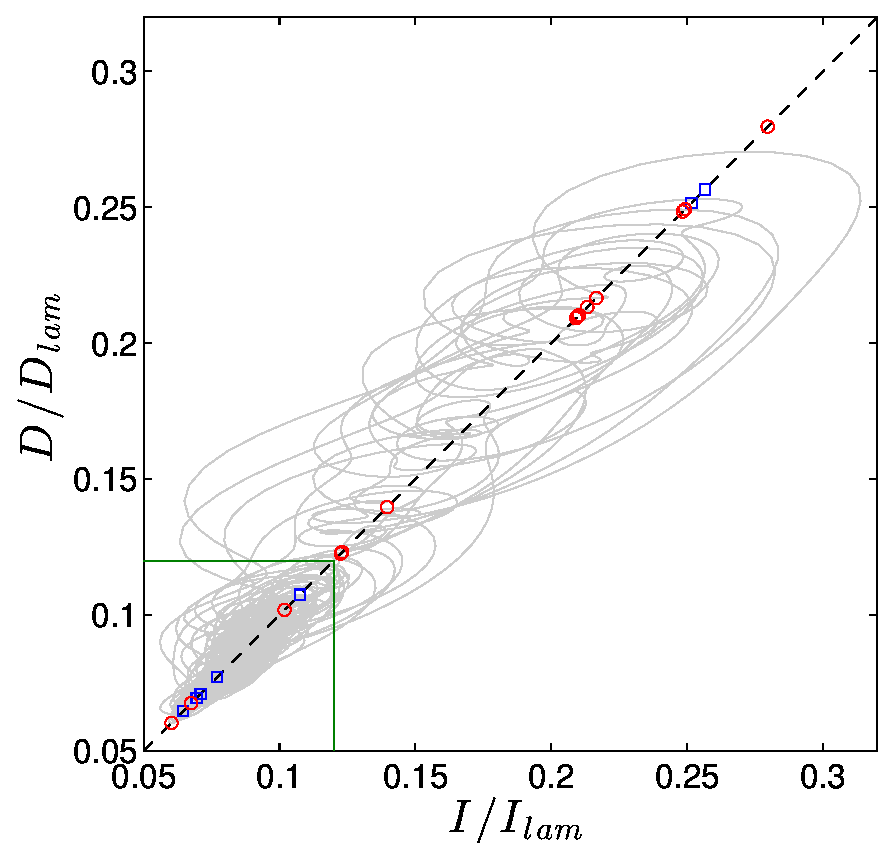
\includegraphics[width=.75\textwidth]{ID_R40}		
\caption{$\mbox{Re}=40$. Gray: Ergodic trajectory. Black star: initial condition for the
ergodic trajectory. Dashed line: $I=D$ line. Dots: Equilibria shown in
\reffig{fig:Kol_R40_E3}.}
\label{fig:ID_R40}
\end{figure}
}
	
\MMFpost{2015-05-05}{Figures \ref{fig:kol_R100_EQ}: Equilibrium for $Re=100$.
	\begin{figure}
		\centering
		(a)\includegraphics[width=.45\textwidth]{Kol_R100_n256_vort_E2}		
		(b)\includegraphics[width=.45\textwidth]{Kol_R100_n256_vort_E4-2sin}
		\caption{$\mbox{Re}=100$ and resolution $256\times 256$. (a) Initial condition
		$\mathbf u(x,y)=(2\cos(2y),2\cos(2x))$ converged to
			equilibrium with residue $6\times 10^{-8}$. (b) Initial condition
			$\mathbf u(x,y)=(\sin(4y),4.5\sin(2x))$ converged to
			equilibrium with residue $1\times 10^{-9}$.}
		\label{fig:kol_R100_EQ}
	\end{figure}
}

\MMFpost{2015-05-05}{\refFig{fig:kol_R80_E2}(b): New equilibrium at $Re=80$ and
\refFig{fig:kol_R60_E1}(c,d): New equilibrium at $Re=60$.
}

\MMFpost{2015-05-04}{Figures \ref{fig:kol_R60_E1}(b) and \ref{fig:kol_R80_E2}:
	New equilibria for $\mbox{Re}=60$ and $80$.
	\begin{figure}
		\centering
        (a)\includegraphics[width=.45\textwidth]{Kol_R80_n256_vort_E2}
        (b)\includegraphics[width=.45\textwidth]{Kol_R80_n256_vort_E2-1}
		\caption{$\mbox{Re}=80$ and resolution $256\times 256$. (a) The adjoint-Newton
		hybrid with initial condition $\mathbf u(x,y)=(2\cos(2y),2\cos(2x))$ converged to
		equilibrium with residue $4\times 10^{-8}$. (b) Initial condition $\mathbf
		u(x,y)=(2\cos(2y),2\cos(x))$ with residue $9\times 10^{-9}$.}
		\label{fig:kol_R80_E2}
	\end{figure}
}	
	
\MMFpost{2015-05-03}{Predrag, could you please create a paper template for the adjoint
method. I'll start filling it up as we go. Most of the theory is
in place, so I can start writing that part immediately.
}
\MMFpost{2015-05-01}{\refFig{fig:kol_R60_E1}: Equilibrium solution for the Kolmogorov
flow at $Re=60$ computed by the adjoint equation.
\begin{figure}
	\centering
	(a)\includegraphics[width=.45\textwidth]{Kol_R60_n128_vort_E1}
    (b)\includegraphics[width=.45\textwidth]{Kol_R60_n256_vort_E2}\\
    (c)\includegraphics[width=.45\textwidth]{Kol_R60_n128_vort_E2-1}
    (d)\includegraphics[width=.45\textwidth]{Kol_R60_n128_vort_E3}
	\caption{$\mbox{Re}=60$ (a) The adjoint equation integrated with initial condition
	$\mathbf u(x,y)=(2\cos(y),2\cos(x))$ for $10^4$ time units (took 2 minutes) then
	switched to Newton-GMRES to reduce the residue to $4\times 10^{-13}$ after $8$
		iterations. Resolution $128\times 128$. (b) The initial
		condition was $\mathbf u(x,y)=(2\cos(2y),2\cos(2x))$ and resolution $256\times
		256$. (c) The initial condition was $\mathbf u(x,y)=(2\cos(2y),2\cos(x))$ and
		resolution $128\times 128$ converged with residue $3\times 10^{-8}$. (d) Initial
		condition $\mathbf u(x,y)=(2\cos(3y),2\cos(3x))$ and resolution $128\times 128$
		converged with residue $1\times 10^{-8}$.}
	\label{fig:kol_R60_E1}
\end{figure}
}
	
\MMFpost{2015-04-22}{I contacted Rich Kerswell regarding the equilibrium solutions I find
for Kolmogorov flow but they did not find. As I suspected, they look for equilibria using
recurrences. As a result, they miss all the equilibria in the shift-invariant subspaces.
I copy the relevant part of his response to my email:

Rich Kerswell: ``I think the quick answer to your question is we didn't find many
equilibria in Chandler \& Kerswell by the approach taken there i.e. recurrent flow
analysis."
}

\MMFpost{2015-04-21}{There seems to be a zoo of shift-invariant equilibria. See
\reffig{fig:Kol_R40_E3}
\begin{figure}
	\centering
	(a)\includegraphics[width=.45\textwidth]{Kol_R40_n128_vort_E1}
	(b)\includegraphics[width=.45\textwidth]{Kol_R40_n128_vort_E2}\\
	(c)\includegraphics[width=.45\textwidth]{Kol_R40_n128_vort_E2-1}
	(d)\includegraphics[width=.45\textwidth]{Kol_R40_n128_vort_E3}
	(e)\includegraphics[width=.45\textwidth]{Kol_R40_n128_vort_E2sin}
    (f)\includegraphics[width=.45\textwidth]{Kol_R40_n128_vort_E4-1sin}
	\caption{$Re=40$ and resolution $128^2$.
		(a) Initial condition $\mathbf
		u(x,y)=(2\cos(y),2\cos(x))$ converged with residue $5\times 10^{-13}$.
		(b) Initial condition $\mathbf u(x,y)=(2\cos(2y),2\cos(2x))$ converged with
		residue $1\times 10^{-13}$.
		(c) Initial condition $\mathbf
		u(x,y)=(2\cos(2y),2\cos(x))$ converged with residue $1\times 10^{-9}$
		(d) Initial condition
		$\mathbf u(x,y)=(2\cos(3y),2\cos(3x))$ converged with residue $4\times 10^{-13}$.
		(e) Initial condition
		$\mathbf u(x,y)=(\sin(2y),\sin(2x))$ converged with residue $4\times 10^{-9}$.
		(f) Initial condition
		$\mathbf u(x,y)=(0.5\sin(4y),3\sin(x))$ converged with residue $2\times 10^{-9}$.
		}
	\label{fig:Kol_R40_E3}
\end{figure}
\begin{figure}
	\centering
	(g)\includegraphics[width=.45\textwidth]{Kol_R40_n128_vort_E23-23}
    (h)\includegraphics[width=.45\textwidth]{Kol_R40_n128_vort_E9}
    (i)\includegraphics[width=.45\textwidth]{Kol_R40_n128_vort_E10}
    (j)\includegraphics[width=.45\textwidth]{Kol_R40_n128_vort_E12}
    (k)\includegraphics[width=.45\textwidth]{Kol_R40_n128_vort_E15}
	\caption{Continued from \reffig{fig:Kol_R40_E3}. $Re=40$ and resolution $128^2$.
		(g) Initial condition $\mathbf
		u(x,y)=(\sin(2y)+\sin(3y),2\sin(2x)+2\sin(3x))$ converged with residue
		$5\times 10^{-9}$. (h) Initial condition $u(x,y)=(\sin(y),\cos(3x))$ converged
		with residue $2.4\times 10^{-10}$ (i) Initial condition
		$u(x,y)=(\sin(y),\cos(2x))$ converged
		with residue $8\times 10^{-11}$. (j) Initial condition
		$u(x,y)=(\sin(2y),\cos(x))$ converged
		with residue $2\times 10^{-10}$.
		(k) Initial condition
		$u(x,y)=(\sin(2y),\cos(x))$ converged
		with residue $1.5\times 10^{-9}$, only Newton-GMRES was used.
			}
\end{figure}
}

\MMFpost{2015-04-21}{\refFig{fig:Kol_R40_E2}: A new equilibrium solution of Kolmogorov
flow that Chandler \& Kerswell (2013) did not find (or did not report).
\begin{figure}
	\centering
	(a)\includegraphics[width=.45\textwidth]{Kol_R40_n128_vort_E2_t0}\\
	(b)\includegraphics[width=.45\textwidth]{Kol_R40_n128_vort_E2_adj}
    (c)\includegraphics[width=.45\textwidth]{Kol_R40_n128_vort_E2}
	\caption{A new equilibrim solution of the Kolmogorov flow for $\mbox{Re}=40$. (a)
	Initial condition for
	the adjoint equation: $\mathbf u(x,y)=(2\cos(2y),2\cos(2x))$. (b) The solution of the
	adjoint equation at time $t=4\times 10^{4}$ (took almost $4$ minutes). (c) The
	solution of the adjoint was used as the initial guess in Newton-GMRES which converged
	after $9$ iterations with residue $10^{-13}$. Note that the solution is in the
	shift-invariant subspace.}
	\label{fig:Kol_R40_E2}
\end{figure}
}
\MMFpost{2015-04-21}{\refFig{fig:Kol_R40_E1}: First equilibria of the Kolmogorov flow
found
using a hybrid of the adjoint method and the Newton-GMRES iterations.

The Kolmogorov flow
\begin{equation}
\partial_t \mathbf u = -\mathbf u\cdot\nabla\mathbf u -\nabla p
+\frac{1}{\mbox{Re}}\Delta \mathbf u + \sin (4y) \mathbf e_1,\quad \nabla\cdot \mathbf
u=0,
\label{eq:kolmogorov}
\end{equation}
is solved with periodic boundary conditions in $x$ and $y$ on the domain $(x,y)\in
[0,2\pi]\times [0,2\pi]$.
\begin{figure}
	\centering
	(a)\includegraphics[width=.40\textwidth]{Kol_CK13_E1}
	(b)\includegraphics[width=.47\textwidth]{Kol_R40_n128_vort_adj+newton}
	\caption{(a) Equilibrium E1 found by Chandler \& Kerswell, JFM 722 (2013) (b) The
	same equilibrium found by adjoint equation integrated for $4\times 10^4$ time units
	(takes approximately $3$ minutes) plus 7 iterations of Newton-GMRES to decrease the
	$L^2$ error to $5\times 10^{-13}$. Here, $\mbox{Re}=40$. Note that panels (a) and (b)
	appear to be related
	by a shift-and-reflect symmetry.}
	\label{fig:Kol_R40_E1}
\end{figure}
}
	
\MMFpost{2015-02-24}{Playing around with Burgers' equation:
\begin{equation}
	\partial_t u + u\,\partial_x u = \nu\, \partial_x^2 u + f(x,u),
	\label{eq:burger}
\end{equation}
where $x\in \mathbb T=[0,2\pi]$, $t\in\mathbb R^+$ and $f(x,u)$ is some forcing. If the
viscosity $\nu>0$ is large enough the solutions remain smooth for all times.

Some properties:
\begin{enumerate}
\item In the absence of forcing, i.e. $f(x,u)=0$, all solutions converge asymptotically
to the trivial solution $u\equiv 0$.	

\item At the first sight, it appears that the forcing term $f(x,u)=\partial_x u$
produces traveling wave solutions. However as it injects zero average energy in the
system, these solutions decay to $u\equiv 0$ (see \reffig{fig:burger}(a)). The zero
energy input is due to the fact that
$$\int_0^{2\pi} u\,\partial_x u\; dx=0.$$

\item Interestingly, fractional-order forcing
$$f(x,u)=\partial_x^{1/2} u,$$
produces self-sustaining traveling waves (see \reffig{fig:burger}(b)).
\end{enumerate}
\begin{figure}
	\centering
	(a)\includegraphics[width=.45\textwidth]{burger_uxForcing}
	(b)\includegraphics[width=.45\textwidth]{burger_fracForcing}
	\caption{Burgers equation with $\nu = 0.1$. (a)  Forcing $f(x,u)=0.5\,\partial_x u$
	(b) Forcing $f(x,u)=0.5\,\partial_x^{1/2} u$.}
	\label{fig:burger}
\end{figure}
}

    \PCpost{2015-01-24}{
As I'm writing up the {\em Life in extreme dimensions} section of
ChaosBook \texttt{flows.tex}, I have found other interesting references,
for example J. Hopcroft and R. Kannan\rf{HopKan14} and
\HREF{https://www.cs.cmu.edu/~venkatg/teaching/CStheory-infoage/} {Ravi
Kannan}'s course.
One might want to scan through
\HREF{http://sankhya.isical.ac.in/search/64a2/64a2031.pdf} {Wegman and
Solka}\rf{WegSol02} approach to visualizing high-dimensional data.
There is also an interesting mathoverflow.org
\HREF{http://mathoverflow.net/questions/25983/intuitive-crutches-for-higher-dimensional-thinking}
{thread}.
    }

    \PCpost{2014-11-10, 2015-01-11}{                            \inCB
I love it. Flaschka's notes are a very high quality solution set to
\refexer{exer:2vecOrthog} {\em In high dimensions any two vectors are
(nearly) orthogonal} that Sara and I wrote up for Xiong, Burak and
Mohammad, in hope that they would do it. Once one does it, one
understands why {\fFslice} give Predrag ulcers...

If you write it up, please enter the solution into solutions in
\refchap{c-PDEs}. I refer to it in the chapter \texttt{flows.tex} (so far
unwritten) section \emph{Life in extreme dimensions}, and the the new set
of videos for
\\
 \wwwcb{/course1/Course1w1.html}.

Sooner, rather than later I (or some combination of us) should add this
section to \texttt{flows.tex}...
    }


    \MMFpost{2015-01-10}{                            \inCB
I came across the very interesting lecture notes by Hermann Flaschka on
\emph{Some geometry in high-dimensional spaces}. Here is
\HREF{http://math.arizona.edu/~flaschka/Topmatter/527files/concentration.pdf}
{the link}. I'm learning a lot from it and will blog if something
relevant is found.
    }

\MMFpost{2014-12-12}{
Each relative equilibrium of modified perturbed KS has its own domain of attraction. Depending on which domain an initial condition falls in, the solution converges to the corresponding equilibrium. \reffig{fig:modPertKS_L32pi_01} shows that starting from a different initial condition, the modified perturbed KS converges to a different relative equilibrium. To obtain all relative equilibria, we need a smart way to distinguish their domains of attractions approximately.
\begin{figure}
	\centering
	\includegraphics[width=.48\textwidth]{KS_L32pi_icRand_3e0_01}
	\includegraphics[width=.48\textwidth]{KS_L32pi_icRand_3e0_profile_01}
	\caption{$\tilde L=L/2\pi=16$. Same as the right panel of \reffig{fig:modPertKS_L32pi} starting from a different initial condition.}
	\label{fig:modPertKS_L32pi_01}
\end{figure}
}
	
\MMFpost{2014-12-12}{My guess for the failure of the \emph{perturbed KS} equation \refeq{eq:pertKS} was that in the Fourier space it contains terms up to the order $+k^8$ where $k$ is the wavenumber. This introduces highly unstable modes that the numerical integrator is not able to resolve.
	
The $k^8$-term comes from the fourth-order derivative $-[F(u)]_{xxxx}$ in equation \refeq{eq:pertKS}. So, I decided to neglect this term and solve the \emph{modified perturbed KS} equation:
\begin{equation}
u_t=F_\epsilon(u):=F(u)+\epsilon\{-F(u)u_x-u[F(u)]_x-[F(u)]_{xx} \} ,\quad x\in[0,L].
\label{eq:modPertKS}
\end{equation}

Interestingly, this crude modification seems to work. \reffig{fig:modPertKS_L32pi} compares a solution of KS \refeq{eq:KS} and the solution of the modified perturbed KS \refeq{eq:modPertKS} starting from the {\bf same initial condition} $u(x,0)$. While the solution of KS is turbulent, the solution of the modified perturbed KS converges to a relative equilibrium.

The relative equilibria of perturbed KS should be close to those of KS. To check this, I take the solution of modified perturbed KS at time $t=400$ and use it as initial condition for KS. Figure \ref{fig:modPertKS_L32pi_restart} shows that in fact the relative equilibrium of modified perturbed KS is close to a relative equilibrium of KS.
\begin{figure}
		\centering
		\includegraphics[width=.48\textwidth]{KS_L32pi_icRand_eps0e0}
		\includegraphics[width=.48\textwidth]{KS_L32pi_icRand_eps3e0}
		\caption{$\tilde L=L/2\pi=16$ (i.e. $L=32\pi$) {\bf Left:} Solution of KS equation \refeq{eq:KS}. {\bf Right:} Solution of modified perturbed KS equation \refeq{eq:modPertKS} with $\epsilon=3$.}
		\label{fig:modPertKS_L32pi}
\end{figure}
%
\begin{figure}[h!]
	\centering
	\includegraphics[width=.48\textwidth]{KS_L32pi_icRestart_0e0}
	\includegraphics[width=.48\textwidth]{KS_L32pi_icRestart_3e0}
	\caption{$\tilde L=L/2\pi=16$. {\bf Left:} Solution of KS \refeq{eq:KS} starting from $u_0(x)=u(x,t=400)$ where $u(x,t)$ is the solution shown in the right panel of \reffig{fig:modPertKS_L32pi}. The solution follows a relative equilibrium. The instabilities finally take the solution away at around $t=40$. {\bf Right:} The relative equilibrium of modified perturbed KS \refeq{eq:modPertKS} is shown for reference.}
	\label{fig:modPertKS_L32pi_restart}
\end{figure}
}
\MMFpost{2014-12-09}{To Predrag: I tried the ``fast direct method" on KS to converge to its \reqva. I failed! So, here I document what I did. Maybe I'm making a mistake.

Consider the Kuramoto--Sivashinsky (KS) equation with periodic boundary conditions:
\begin{equation}
u_t=F(u):=-uu_x-u_{xx}-u_{xxxx},\quad x\in[0,L].
\label{eq:KS}
\end{equation}
Figure \ref{fig:KS_L32pi} shows a typical solution with $L=32\pi$. (I played around with the length $L$ and tried various sizes, including $L=22$).

By analogy with the finite dimensional case, I add a small ``acceleration term" to KS, i.e., solve
\begin{equation}
u_t=F_\epsilon(u):=F(u)+\epsilon u_{tt},\quad x\in[0,L],\quad 0<\epsilon\ll 1.
\label{eq:pertKS}
\end{equation}
Taking a time derivative of KS, it follows that
$$u_{tt} = -F(u)u_x-u[F(u)]_x-[F(u)]_{xx}-[F(u)]_{xxxx},$$
which coincides with the G\^ ateaux differential of $F$ at $u$ in direction $u_t=F(u)$, that is
$$u_{tt} = dF(u;u_t).$$

I solved \refeq{eq:pertKS} numerically starting from various initial conditions and various parameter values $\epsilon$. And with no luck in converging to a \reqva. Remember that in the case of 2-mode Porter-Knoblock and complex Lorenz, I converged to the \reqva\ starting from arbitrary initial conditions.
\begin{figure}
	\centering
	\includegraphics[width=.7\textwidth]{KS_L32pi_ic2}
	\caption{A typical solution of Kuramoto-Sivashinsky equation with domain size $L=32\pi$.}
	\label{fig:KS_L32pi}
\end{figure}
}

\MMFpost{2015-01-14}{Applying the stabilizing vector field \refeq{eq:u} to the Henon map
	\begin{equation*}
	(x,y)\mapsto (1-ax^2+y,by)
	\end{equation*}
	with $a=1.4$ and $b=0.3$. Define $\mathbf x=(x,y)$ and denote the Henon map by $f$: $\mathbf x\mapsto f(\mathbf x)$.
	
	\refFig{fig:henon_stabilizingFlow}(a) shows the convergence of a trajectory of the stabilizing flow $$u(\mathbf x)=-[\nabla v(\mathbf x)]^{-1}v(\mathbf x)$$ to a cycle of order $n=20$. \refFig{fig:henon_stabilizingFlow}(b) shows the evolution of the error
	$$\|\mathbf x(t)-f^n(\mathbf x(t))\|,$$
	with $n=20$ where $\mathbf x(t)$ is a trajectory of $u$ and $\|\cdot\|$ denotes the Euclidean norm on $\mathbb R^2$.
	\begin{figure}
		(a)\includegraphics[width=.48\textwidth]{henon_N20_traj}
		(b)\includegraphics[width=.42\textwidth]{henon_N20_error}
		\caption{(a) An order $20$ cycle of the Henon map: $f^{20}(\mathbf x)=\mathbf x$. The initial condition $(0,0)$ for the stabilizing vector field $u$ is shown by a blue square. The blue curve shows the corresponding trajectory $\mathbf x(t)$. The blue dots show $20$ iterations of the Henon map starting from the end point of the trajectory $\mathbf x(t)$. (b) The evolution of the error $\|\mathbf x(t)-f^n(\mathbf x(t))\|$ with $n=20$. The error decreases monotonically at an exponential rate.}
		\label{fig:henon_stabilizingFlow}
	\end{figure}
}

\MMFpost{2015-01-14}{The vector field \refeq{eq:u} can be derived from an equivalent, norm-dependent formulation:
	
	Consider a given vector field $v:U\rightarrow \mathbb R^m$ where $U\subset\mathbb R^m$. The equilibria, $x\in U$ such that $v(x)=0$, are the minimizers of the functional
	$$\mathcal F(x)=\|v(x)\|^2,$$
	where $\|\cdot\|$ is the Euclidean norm. Let $\delta x\in\mathbb R^m$ and $\|\delta x\|\ll 1$. Then
	$$\mathcal F(x+\delta x)=\mathcal F(x)+2\langle v(x),\nabla v(x)\delta x\rangle +\mathcal O(\|\delta x\|^2).$$
	To ensure that $\mathcal F(x+\delta x)\leq \mathcal F(x)$ for small $\delta x$, it is sufficient to have
	$$\nabla v(x)\delta x=-v(x),$$
	or equivalently
	$$\delta x=-[\nabla v(x)]^{-1}v(x).$$
	Equation \refeq{eq:u} is the infinitesimal version of the above `Newton-Raphson' iteration.
}

\MMFpost{2015-01-13}{The fictitious vector field $u(x)=-\nabla v(x)\, v(x)$ described below can also be used to find fixed points and cycles of maps.
	
	Consider the map $x\mapsto f(x)$ defined over $\mathbb R^m$. For finding fixed points $x=f(x)$, we let $v(x)=x-f(x)$ where $\nabla v(x) = I_m-\nabla f(x)$.
	
	For a cycles of order $n$, where $x=f^n(x)$, we let $v(x)=x-f^n(x)$ and hence
	$$\nabla v(x) = I_m-\nabla f(f^{n-1}(x))\nabla f(f^{n-2}(x))\cdots\nabla f(x).$$
	
	For large $n$, the numerical accuracy can be improved using an idea from Chaos Book. Namely, extend the system by a vector $(x_1,x_2,\cdots,x_n)\in\mathbb R^{n\times m}$ such that $x_2=f(x_1)$, $x_3=f(x_2)$, ..., $x_1=f(x_{n})$, where $x_i\in\mathbb R^m$.
}

	\MMFpost{2014-11-29}{
One more example for the stabilizing flow of equilibria as explained below, i.e., $u =-(\nabla v)^{-1} v$.

Consider the pendulum
\begin{equation}
\dot x_1= x_2,\quad \dot x_2=-\sin(x_1).
\label{eq:pendulum}
\end{equation}
That is $v(x_1,x_2)=(x_2,-\sin(x_1))$. Therefore, we have
$$u(x_1,x_2)=(-\tan(x_1),-x_2).$$

\reffig{fig:pendulum} shows the trajectories of $u$ which take initial conditions to the fixed points of $v$: $x_1=0,\pm\pi$, $x_2=0$.

Note that the equilibria of $v$ all become \emph{stable} equilibria of $u$ with the following domains of attraction:
$$\mbox{Domain of attraction of}\ (0,0) = \{-\pi/2<x_1<\pi/2\}\times \{x_2\in\mathbb R\}$$
$$\mbox{Domain of attraction of}\ (\pi,0) = \{\pi/2<x_1\leq\pi\}\times \{x_2\in\mathbb R\}$$
$$\mbox{Domain of attraction of}\ (-\pi,0) = \{-\pi\leq x_1<-\pi/2\}\times \{x_2\in\mathbb R\}$$

Also, note that $u$ is not defined on $x_1=\pm\pi/2$ since $\nabla v$ is singular on these lines. These singularity lines separate the domains of attraction of the equilibria of $u$.
\begin{figure}[h!]
\centering
\includegraphics[width=.7\textwidth]{pendulum_stabilizingFlow_02}
\caption{Gray color: Solutions of the pendulum equation \refeq{eq:pendulum}. Black dots: The equilibria $x_1=0,\pm\pi$, $x_2=0$. Blue color: The trajectories of the stabilizing vector field $u$. Red lines: Singularities of $u$ which divide the domains of attraction of the equilibria.}
\label{fig:pendulum}
\end{figure}
}
				
	\MMFpost{2014-11-29}{There are many ways to search for the equilibria of a differential equation
$$\dot x=v(x),\quad x\in\mathbb R^n.$$
They include
\begin{enumerate}
\item Finding the zeros of the algebraic equation $v(x)=0$, using some Newton method.
\item Finding the solutions of $f^t(x)=x$ for all $t$, where $f^t$ is the solution map of the differential equation. This is sometimes done by finding the minimizers of $\|f^t(x)-x\|^2$ for all $t$. This assumes a norm $\|\cdot\|$ and then uses Newton iterations or Newton descent method (introducing a fictitious time $\tau$).
\end{enumerate}

Here is a third method which combines the two approaches above but does NOT use a norm. The problem can be formulated as follows: Find a dynamical system $g^\tau$ such that $\lim_{\tau\rightarrow\infty}v(g^\tau(x))=0$ for all $x$.

To find such a flow $g^\tau$, define
$$\phi(\tau;x)=v(g^\tau(x)),$$
for an arbitrary $x\in\mathbb R^n$. Constrain $g^\tau$ such that $\lim_{\tau\rightarrow\infty}\phi(\tau;x)=0$. This constraint can be imposed in several ways. One is to require $\phi(\tau;x)$ to satisfy the following ODE:
\begin{equation}
\partial_\tau\phi(\tau;x)=-\phi(\tau;x),
\label{eq:const}
\end{equation}
whose solutions are $\phi(\tau;x)=\phi(0;x)\exp(-\tau)=v(x)\exp(-\tau)$.

Now, from definition of $\phi$ we have $\partial_\tau\phi = \nabla v(g^\tau(x))\partial_\tau g^\tau(x)$. If $u$ is the infinitesimal generator of $g^\tau$, i.e. $\partial_\tau g^\tau(x)=u(g^\tau(x))$, we get $\partial_\tau\phi=\nabla v(g^\tau(x))u(g^\tau(x))$. This, together with constraint \refeq{eq:const}, implies
$$ \nabla v(y)u(y)=-v(y),\quad y=g^\tau(x).$$
If $\nabla v$ is (almost everywhere) invertible, $u$ is explicitly defined in terms of $v$ as
\begin{equation}
u =-(\nabla v)^{-1} v.
\label{eq:u}
\end{equation}

{\bf Examples:} Consider the linear saddle
$$ \dot x_1 = x_1,\quad \dot x_2=-x_2,\quad x_1,x_2\in \mathbb R$$
and the harmonic oscillator
$$\dot x_1 =x_2,\quad \dot x_2=-x_1,\quad x_1,x_2\in \mathbb R.$$
The first equation has a hyperbolic fixed point at the origin while the second equation has a center fixed point at the origin. Using \refeq{eq:u}, the auxiliary vector field $u$ for both the saddle and the harmonic oscillator is
$$u(x_1,x_2)=(-x_1,-x_2),$$
whose flow $g^\tau$ takes any initial condition $x$ to the equilibrium at the origin, exponentially fast.

In fact, for any smooth linear flow $v(\mathbf x)=A\mathbf x$ with $\mathbf x\in \mathbb R^n$, we have $u(\mathbf x)=-A^{-1} v=-A^{-1}A\mathbf x= -\mathbf x$. The flow of $\dot{\mathbf x}=u(\mathbf x):=-\mathbf x$ takes any initial condition to the fixed point $\mathbf x=0$.
}

    \PCpost{2014-11-22}{

{\bf A fast explicit method for computing unstable invariant
        solutions of high-dimensional dynamical systems}

{\bf Desiderata}:
Find a method that determines time-invariant unstable solutions (or their
neighborhoods) of a given dynamical system without imposing any
extraneous norm on the \statesp\ of the system. By that one means a
method other than a Newton method or optimization methods that minimize
squares of errors computed with an externally imposed norm, not intrinsic
to dynamics.

{\bf Proposal}:
Modify the flow in the neighborhood of an unstable invariant set with terms
quadratic in the linearized stability exponents, parametrized
by $M$ small parameters $\epsilon_j$, one for each distinct positive real
part \eigRe[j] of a stability exponent
$\eigExp[j]=\eigRe[j]\pm\eigIm[j]$, in such a way that all stability
exponents of the modified flow are contracting, and the flow converges to
an $\epsilon$-nearby invariant set.


{\bf Discussion}:
In common iterative schemes or differential equations set up to converge
to desired invariant sets, one always (?) introduces an extra fictitious
time (or the Newton iteration number), see ChaosBook.tex Sect.~29.1
\HREF{http://www.streamsound.dk/book1/chaos/chaos.html\#613/z}
{\emph{Fictitious time relaxation}} and
\refrefs{CvitLanCrete02,lanVar1,LCC06,Lan:Thesis}. The novelty here is
that the equations of motion themselves are modified, with no
introduction of a fictitious time, and without introducing a norm to
measure the distance to the desired solution. Only linear stability and
directional (Jacobi) derivatives are used.

I think the essence of Mohammad's approach is not in using curvature of
trajectories, but in modifying the flow by adding to it terms quadratic in
eigenvalues of the {\stabmat} {\Mvar} in such a way that the modified
flow converges to a  nearby stable invariant set. Maybe you can think of it
as follows:

(text clipped from ChaosBook.tex Sect.~4.4
\HREF{http://www.streamsound.dk/book1/chaos/chaos.html\#102/z}
{\emph{Stability of flows}}):

The finite time \jacobianM\ $\jMps^\zeit$ is related to the {\stabmat}
{\Mvar} by the formal integral along a trajectory,
\beq
\jMps^\zeit_{ij}(\xInit)
= \left[ {\bf T} e^{ \int_0^\zeit d\tau \Mvar (\ssp(\tau)) } \right]_{ij}
\,,
\label{hodes}
\eeq
where ${\bf T}$ stands for time-ordered integration, {defined} as
the continuum limit of successive multiplications
\beq
\jMps^\zeit =
\lim_{m \to \infty}\prod_{n=m}^1
\left(\matId + \delta t \Mvar(\ssp_n) \right)
\ee{Jprod1}
For nonlinear dynamical
systems, the local rate of neighborhood distortion $\Mvar(\ssp)$
depends on where we are along the trajectory. The linearized
neighborhood is deformed along the flow, and the $m$
discrete time-step approximation to $\jMps^\zeit$ is therefore given
by the above product,
where $\delta \zeit = {(t-t_0)/ m}$, and $\ssp_n=\ssp(t_0+n\delta \zeit)$.
Indexing of the products indicates that the successive infinitesimal
deformation are applied by multiplying from the left.

For convenience, set $\ssp_0 \to \ssp$, expand \refeq{Jprod1} to order
$\delta t^2$,
\bea
\jMps^{2\delta t}(\ssp) &=&
\matId
+ \delta t  \left(\Mvar(\ssp) + \Mvar(\ssp_1)\right)
+ \, \delta \zeit^2 \Mvar(\ssp)^2 + O(\delta \zeit^3)
    \continue
    &=&
\matId
+ 2 \delta \zeit \, \Mvar(\ssp)
    \ceq
+ \delta \zeit^2 \left( (\vel(\ssp)\cdot \nabla)\Mvar(\ssp)
                 + \Mvar(\ssp)^2\right) + O(\delta \zeit^3)
\label{Jprod2}
\eea
replace $\delta \zeit^2 \to \epsilon\delta t$, modify the original
flow accordingly, and use $\epsilon$ to manipulate local stability.

Dimensionally, $\epsilon$ is time (a decay rate toward the \eqv? see
\refeq{stabExpEpsilon}), so one
might consider non-dimensionalizing it.

If looking for an \eqv, on the \eqv\ $\ssp_\stagn$ of the original flow
the pesky `curvature' term $(\vel(\ssp)\cdot \nabla)\Mvar(\ssp)$
vanishes.

{\bf Marginal stability exponents} have to be removed. For \reqva\ this
is achieved by studying eigenvalues of $(\Mvar-\velRel\cdot\Lg)$, see
\refeq{ReqvMargEig}. For \po s this is achieved by any local \Poincare
section, and for \rpo s and hyperbolic $N$-tori
by any (local or global) symmetry reduction
together with any local \Poincare section.

{\bf A single real unstable eigen-direction case}.
If the $\ssp_\stagn$ has an unstable eigenvector
$\jEigvec[j](\ssp_\stagn)$ with a real unstable stability exponent
$\eigExp[j]>0$, at a nearby $\ssp$ they will both pick up terms of order
$\delta \zeit$. Perhaps one can compute the corresponding eigenvector
$\jEigvec[j](\ssp,\delta \zeit)$ at the guess point $\ssp$ and use
the $(\epsilon<0)$-modified real stability exponent $\eigExp[j]+\epsilon
(\eigExp[j])^2$ to reverse flow along 1\dmn\
$\jEigvec[j](\ssp_\stagn,\delta \zeit)$ to now go towards the
$\epsilon$-nearby \eqv\ $\ssp_{\stagn,\epsilon}$.

{\bf A complex pair, 2\dmn\ unstable eigen-plane case}. See below.

{\bf A finite number of expanding directions}.
{\stabmat} {\Mvar} can be brought to a pimply upper-triangular form (a
pimple for each complex pair or other subspace with a single real part of
the stability exponent\rf{DingCvit14}). The unstable flow can be
`reversed' by a range of values for $\epsilon_i$ parameters, one for each
of projections on 1, 2, m\dmn\ subspaces of spanned by sets the
degenerate eigenvectors of the $\epsilon_i$-distorted flow.
    }

	\PCpost{2014-11-22}{
If $ v(x)$ is autonomous, not time dependent, and
\[
a(\ssp)= \frac{d \vel(\ssp)}{d \zeit}
   = \nabla \vel(\ssp)\vel(\ssp) = \Mvar(\ssp)\vel(\ssp)
\]
is the `acceleration', maybe we should double the number of coordinates
to $[y,u]$, $y=\ssp-\epsilon \vel$, and integrate the pair of first
order ODEs,
\bea
{\dot y}_j(\zeit) &=& \vel(y,u)_j
    \continue
{\dot u}_j(\zeit)
 &=& \frac{d \vel_j}{d \ssp_k}\,\vel(y,u)_k
  = \Mvar(y,u)_{jk}\,\vel(y,u)_k
\,,
\eea
from initial condition $[y(0),u(0)]= [\ssp(0),\vel(\ssp(0))]$. Not sure
all this makes sense: it puts \eqv\ at the origin, which cannot be right.
    }


	\PCpost{2014-11-22}{
For \cLe\ unstable \eqv\ at the origin $\lambda_5=-2.67$ presumably has
$z$-axis as its eigenvector. It is an invariant subspace, no need to
discuss it further. I am not sure about your two complex eigenvalue pairs
$\eigExp[1,2]$ and $\eigExp[3,4]$. Remember that they have to be computed
in the symmetry-\reducedsp, as eigenvalues of $(\Mvar-\velRel\cdot\Lg)$,
see \refeq{ReqvMargEig}. We have computed them zillion places, I just
cannot remember off the bat where: ChaosBook? Siminos thesis? Siminos or
Froehlich blogs? \refrefs{SiCvi10,FrCv11}? I seem to vaguely remember one
of them being real, but am not sure. If so,  $(\epsilon<0)$-modified real
stability exponent of my post above would be the right thing. If you have
only one unstable direction (or complex pair) being sloppy about the
choice of contracting direction is OK.
    }

	\MMFpost{2014-11-20}{To Predrag:
Following our discussion today-- \cLe\ has an unstable
{\eqv} at the origin. I have not been able to converge to it for any
$\epsilon>0$ using $v_\epsilon(x)=v(x)+\epsilon (\nabla v(x)) v(x)$. The
eigenvalues of the {\stabmat} {\Mvar} at the origin are:
\[
  \lambda_{1,2}=11.83\pm i 0.063,\quad
  \lambda_{3,4}=-22.83\pm i 0.037,\quad \lambda_5=-2.67
  \,.
\]
	That is $S^+_<\neq\emptyset$; hence condition 1 of the theorem below
is violated.
	
However, for $\epsilon<0$, I do converge to the origin which is good. So,
maybe we need to check both positive and negative $\epsilon$.
}

	\MMFpost{2014-11-18}{ Here is what I have so far. I do it for {\eqv} but a
similar result holds for relative {\eqv} after symmetry reduction. Looking forward
to your opinions/suggestions...

Consider the differential equation $\dot x=v(x)$ on $\mathbb R^n$ which has a fixed point
$x_0$, i.e., $v(x_0)=0$. Then $x_0$ is also a fixed point of the perturbed equation
$\dot x = v_\epsilon(x)$ where $v_\epsilon(x)=v(x)+\epsilon a(x)$ with
$a(x)=\nabla v(x)v(x)$.

Linear stability matrix: Let $A:=\nabla v(x_0)$ and $A_\epsilon:=\nabla v_\epsilon (x_0)$.
For any $x\in\mathbb R^n$, we have
$$ \nabla v_\epsilon(x) = \nabla v(x) + \epsilon [\nabla v(x)]^2 + \epsilon[v(x)\cdot \nabla] \nabla v(x).$$
Substituting $x=x_0$ and using $v(x_0)=0$, we get
$$ A_\epsilon = A + \epsilon A^2$$

Assume $A$ has $n$ distinct eigenvalues
$\lambda_k=\mu_k\pm i\omega_k\in\mathbb C$ (w.l.o.g., let $\omega_k\geq0$). Then there is
a basis in which $A$ is block diagonal with blocks
\begin{equation}
\begin{pmatrix}
\mu_k & -\omega_k \\
\omega_k & \mu_k
\end{pmatrix}.
\end{equation}
The block is a $1\times 1$ scalar matrix for real eigenvalues $\lambda_j=\mu_j$.

In the same basis, $A_\epsilon$ is also block diagonal with blocks
\begin{equation}
\begin{pmatrix}
\mu_k+\epsilon(\mu_k^2-\omega_k^2) & -\omega_k(1+2\epsilon\mu_k) \\
\omega_k(1+2\epsilon\mu_k) & \mu_k+\epsilon(\mu_k^2-\omega_k^2)
\end{pmatrix}.
\end{equation}
Therefore, the real parts of the eigenvalues of $A_\epsilon$ are
\beq
\mu_k+\epsilon(\mu_k^2-\omega_k^2)
\,.
\ee{stabExpEpsilon}
For the point $x_0$ to be a stable fixed point of $\dot x=v_\epsilon(x)$,
we need all the above numbers to be negative.

{\bf Notation:} For determining the conditions of stability of $x_0$, the following
notation will become handy. Let $\{1,2,\cdots,n\}=S^+\cup S^-$ where
$$S^+=\{1\leq k\leq n\ |\ \mu_k\geq 0\},$$
$$S^-=\{1\leq k\leq n\ |\ \mu_k< 0\}.$$
Further split $S^+$ as $S^+=S^+_>\cup S^+_<$ where
$$S^+_>=\{k\in S^+\ |\ \omega_k>\mu_k\},$$
$$S^+_<=\{k\in S^+\ |\ \omega_k\leq\mu_k\}.$$
Similarly split $S^-$ as $S^-=S^-_>\cup S^-_<$ where
$$S^-_>=\{k\in S^-\ |\ \omega_k\geq|\mu_k|\},$$
$$S^-_<=\{k\in S^-\ |\ \omega_k<|\mu_k|\}.$$

With a little algebra, one arrives at the following result.

{\bf Lemma:}
The inequalities $\mu_k+\epsilon(\mu_k^2-\omega_k^2)<0$ are satisfied for all
$1\leq k\leq n$, if and only if,
\begin{enumerate}
	\item $S^+_< = \emptyset$ and
	\item $\epsilon>0$ satisfies
	$$\max_{k\in S^+_>} \frac{\mu_k}{\omega_k^2-\mu_k^2}<\epsilon<\min_{k\in S^-_<} \frac{-\mu_k}{\mu_k^2-\omega_k^2}.$$
\end{enumerate}

All put together, we get the following result for stabilizability of an unstable
{\eqv}:

{\bf Theorem:} Let $v(x_0)=0$ and $\nabla v(x_0)$ have distinct eigenvalues
$\mu_k\pm i\omega_k$ satisfying
\begin{enumerate}
	\item $S^+_< = \emptyset$ and
	\item $\max_{k\in S^+_>} \frac{\mu_k}{\omega_k^2-\mu_k^2}<\min_{k\in S^-_<} \frac{-\mu_k}{\mu_k^2-\omega_k^2}.$
\end{enumerate}

Then for any $\epsilon$ such that $$\max_{k\in S^+_>}
\frac{\mu_k}{\omega_k^2-\mu_k^2}<\epsilon<\min_{k\in S^-_<}
\frac{-\mu_k}{\mu_k^2-\omega_k^2},$$ the point $x_0$ is an asymptotically
stable {\eqv} of $\dot x=v(x)+\epsilon\nabla v(x) v(x)$.
}

\MMFpost{2014-11-18}{
I agree continuous symmetry is not essential; I was actually motivated by
observing that it works for elliptic fixed points.
}

    \PCpost{2014-11-17}{
I think continuous symmetry is not the essential part of your algorithm,
and if you subtract from the {\stabmat} {\Mvar} the other part of the
Jacobi derivative, you will essentially work in the symmetry-reduced
\statesp.

Now, about \po s. Suppose you make a guess at one by placing your guess
loop $L$ into the \statesp. At every point $\ssp\in L$ there are two
vectors - the dynamical velocity field $\vel(\ssp)$ and the tangent of
your loop $t(\ssp)$. Maybe you can construct the new flow by subtracting
the Jacobi derivative of the two, and that will move all points on your
guess loops toward the true \po? On any \po\ this Jacobi derivative vanishes.

Whatever you do, do not take the square of this local Jacobi derivative,
as that requires a (here unwelcome) norm.
    }



    \PCpost{2014-11-17}{
That settles is.

Curious: if in \reffig{fig:stabCmplxLorenz_hilbertBases})\,(a) you use
the same units on two axes (plot this on a square of size 400$\times$400),
does spiral look isotropic, rather than squashed?

Do you know what the new stability exponents are? My guess would be that
the real part has no obvious relation to the original, unstable one
(perhaps has a linear or square root dependence on small $\epsilon$'s?),
but that the imaginary part is the same as for the original {\eqv},
up to $O(\epsilon)$. I'm guessing this as think your method makes a
weekly positive real part $\eigRe{}$, but the imaginary part $\pm
\eigIm{}$ is far of the real axis and it does not shift much.
    }

    \MMFpost{2014-11-17}{
I liked the Hopf bifurcation idea. But it seems that the trajectory of
the perturbed system does really converge to a point after symmetry
reduction. Here is some evidence for complex Lorenz. I calculate the
trajectory of the perturbed system in the Hilbert polynomial bases,
$(u_1,u_2,u_3,u_4,u_5)$ as given in \rf{SiCvi10}. I plot the $(u_1,u_2)$
projection below, indicating the spiral towards a point (see
\reffig{fig:stabCmplxLorenz_hilbertBases}). Similar observation holds for
other projections (not presented here).

Could there be a tiny circle?! To check this, I also plot $u_1(t)$ and
$u_5(t)$ and observe that they converge to a constant as $t$ increases (I
zoomed in on my screen, they are really constant lines). Same is true for
other $u_k(t)$.
    }
\begin{figure}
	\centering
	\includegraphics[width=.6\textwidth]{u1vu2_stab_cmlxLorenz.pdf}\\
	\includegraphics[width=.45\textwidth]{u1vt_stab_cmplxLorenz.pdf}
	\includegraphics[width=.45\textwidth]{u5vt_stab_cmplxLorenz.pdf}
	\caption{A trajectory of the ``stabilized" complex Lorenz plotted in the Hilbert polynomial basis.}
	\label{fig:stabCmplxLorenz_hilbertBases}
\end{figure}


    \MMFpost{2014-11-16} {
I have done some further analysis that shows that once
you have a (relative) {\eqv} with complex conjugate eigenvalues which satisfy a
a particular condition (similar to spectral gap), the added acceleration
turns it into a stable {\eqv}. This seems in agreement with your intuition.
I'll type these first chance I get. But its connection to the Hopf torus remains unclear
to me. Maybe I get it once I do \refexer{exer:ExactLyap}.
    }

    \PCpost{2014-11-15, 2014-11-22}{
Your algebra is right. If I remember
correctly, the {\cLf} \reqv\ that you are testing his method on has a
complex, spiral-out eigenvalue pair. My next guess then is that your
additional term reins in the expanding spiral by making it fall into an
attractive Hopf limit torus (limit cycle, once your reduce the symmetry).
The additional term is presumably quadratic, which would explain the
large basin of attraction. I've prepared \refexer{exer:ExactLyap}~{\em A
limit cycle with analytic Floquet exponent} for you. For {\cLf} you
should probably first go to the {\fFslice}, compute numerically the
{\reducedsp} \reqv\ point $\sspRed_{\REQV{}{1}}$. Then expand {\stabmat}
$(\Mvar-\velRel\cdot\Lg)$ numerically around $\sspRed_{\REQV{}{1}}$ up
to quadratic order in $(\sspRed-\sspRed_{\REQV{}{1}})$. That might give you
the Hopf normal form. If you do it, please enter the solution into
solutions in \refchap{c-invariants}.
    }


	\MMFpost{2014-11-12}{
		What I derived for $A_\epsilon:=\nabla v_\epsilon$ looks different. I have
		$$\nabla v_\epsilon = \nabla v + \epsilon\left[(v\cdot\nabla) \nabla v + (\nabla v)^2 \right].$$
		Or equivalently,
		$$A_\epsilon = A + \epsilon\left[(v\cdot\nabla) A + A^2 \right].$$
The term $\frac{\pde^2 \vel_{i}}{\pde \ssp_j \pde \ssp_k} \Mvar_{kj}$ you
have doesn't look right to me since after summing over repeated indices
$k$ and $j$, it would be a 1-tensor while it needs to be a 2-tensor. Do
we agree?
		}
    \PCpost{2014-11-10}{
You know the `$\epsilon$' matrix of velocity gradients explicitly. The fun is
that now it involves objects with three indices
\[
(\Mvar_\epsilon)_{ij} = \cdots
    + \epsilon\left(
      \frac{\pde^2 \vel_{i}}{\pde \ssp_j \pde \ssp_k} \Mvar_{kj}
      + (\Mvar^2)_{ij}
      \right)
\,,
\]
if my algebra is right.
		}

	\MMFpost{2014-11-11}{
Yes, this would be a fast preconditioning method for finding the initial
guess for the Newton method. In fact, that is how I found relative
{\eqv} for complex Lorenz and 2-mode PK equations.
		
I have been trying to show analytically, under general conditions, that
the {\stabmat} in the co-moving frame has one marginal direction
and the rest contracting. Doing them numerically for specific examples
would be helpful. I'll do this next. But still a proof would be nice. The
difficulty is that analytically we only know the action of $A_\epsilon$
on the group tangent $t(a)$, as you wrote in Eq. \refeq{inftmInv}.
		}

    \PCpost{2014-11-10}{
Thanks for info: so maybe one could use your method to get
$\mathcal{O}(\epsilon)$-close to the true \reqv, the switch to Newton to
nail it - finding initial guesses for \reqva\ is already a non-trivial
achievement. How about computing --numerically-- the eigenvalues of the
co-moving {\stabmat} \refeq{ReqvMargEig} at your $v_\epsilon=0$
\reqv,
\[
\Mvar_\epsilon - \velRel_\epsilon \cdot \Lg
\,,\qquad
(\Mvar_\epsilon)_{ij} = \pd{\vel_{\epsilon,i}}{\ssp_j}
\,.
\]
That should give you one marginal, rest contracting - also over a
large basin of attraction away from the \reqv\ point.
    }

    \MMFpost{2014-11-10}{
One clarification regarding Predrag's comment below. I modify the
dynamical system $\dot x=v(x)$ to $\dot x=v_\epsilon(x):=v(x)+\epsilon
a(x)$ where $0<\epsilon\ll 1$ and
\[
a(x)=\nabla v(x)v(x) = \Mvar(\ssp)\vel(\ssp)
\]
is the
`acceleration'. This appears to turn unstable \reqv\ of $v$ to
globally attracting \reqv\ of $v_\epsilon$. The two \reqva,
however, do NOT coincide. \Reqva\ of $v_\epsilon$ are
$\mathcal{O}(\epsilon)$-close to those of $v$.
    }


    \PCpost{2014-11-06}{
Mohammad has a new idea on how to find \reqva: he adds a small parameter
$\times$ acceleration term (local curvature of the trajectory) to the
full \statesp\ flow, and that drives any orbit in a large basin of
attraction to a \rpo. Here is my interpretation.

The infinitesimal, Lie algebra $\Group$-equivariance condition is\rf{DasBuch}
\index{group!tangent field}\index{tangent!field, group}
\beq
  \Lg_a \vel(\ssp)  - \Mvar(\ssp) \, \groupTan_a(\ssp) =0
  \,,
\ee{inftmInv}
where $\Mvar_{ij}= {\pde \vel_i}/{\pde \ssp_j}$ is the \stabmat, and
$(\Lg_a)_{ij}$ is the $d$-dimensional representation of generators of continuous
group transformations. The left-hand side of \refeq{inftmInv} is the {\em
Lie derivative} of the dynamical flow field $\vel$ along the direction of
the infinitesimal group-rotation induced flow $\groupTan_a(\ssp)= \Lg_a
\ssp$. The equivariance condition \refeq{inftmInv} states that the two
flows, one induced by the dynamical vector field $\vel$, and the other by
the group tangent field $\groupTan$, commute if their Lie derivatives (or
the `Lie brackets ' or `Poisson brackets') vanish.
    \index{Lie!derivative} \index{Lie!bracket}
    \index{Poisson!bracket}

For a \reqv, the flow and group tangent vectors coincide,
$
\vel(\ssp) = \velRel \cdot \groupTan(\ssp)
\,.$
Dotting the equivariance condition \refeq{inftmInv} by the velocity $c$
(\ie, summing over $\velRel_a \groupTan_a$), we get
\beq
(\Mvar-\velRel\cdot\Lg) \vel =0
\,.
\ee{ReqvMargEig}
In other words, in the co-rotating frame the eigenvalues corresponding to
group tangent are marginal, and the velocity $\vel$ is the corresponding
right eigenvector.

At every point $\ssp \in \pS$ of the equivariant \statesp\ $\pS$ there are two kinds of
vectors: $\vel(\ssp)$ and $\groupTan(\ssp)\,.$ I think that the
acceleration term $\dot{\vel}$ that Mohammad adds to the RHS of
$\dot{\ssp} = \vel(\ssp)$ penalizes a non-vanishing angle between the
two, but exactly vanishes by \refeq{ReqvMargEig} once the trajectory has
descended to a \reqv. There are very few of those, so basins of
attraction are large.

A search for \reqv\ would require rethinking how this would work in a
Poincar\'e section of the equivariant \statesp\ (before constructing a
slice). Such section cuts the \rpo\ torus and is a circle.

If I understand it right, this is an \reqv\ determination method that is
not a Newton method, and that does not depend on any notion of norm, as
the Lie derivative is local and requires no notion of distance. If that
is true, I'm very happy.

(This is modification of a flow is not quite in the spirit of Biham and
Wenzel\rf{afind}, who add a new fictitious time ODE.)
    }

    \PCpost{2014-10-15}{
Added Mohammad Farazmand to the repo.
    }

    \PCpost{2013-10-03}{
Added Greg Byrne and Adam Fox to the repo.
    }

%\begin{figure}
%	\centering
%	(a)\includegraphics[width=.45\textwidth]{Kol_R40_n128_vort_adj+newton}
%	(b)\includegraphics[width=.45\textwidth]{Kol_R40_n128_vort_E2}\\
%	(c)\includegraphics[width=.45\textwidth]{Kol_R40_n128_vort_E2-1}
%	(d)\includegraphics[width=.45\textwidth]{Kol_R40_n128_vort_E3}
%	(e)\includegraphics[width=.45\textwidth]{Kol_R40_n128_vort_E2sin}
%	(f)\includegraphics[width=.45\textwidth]{Kol_R40_n128_vort_E4-1sin}
%	\caption{$Re=40$ and resolution $128^2$.
%		(a) Initial condition $\mathbf
%		u(x,y)=(2\cos(y),2\cos(x))$ converged with residue $5\times 10^{-13}$.
%		(b) Initial condition $\mathbf u(x,y)=(2\cos(2y),2\cos(2x))$ converged with
%		residue $1\times 10^{-13}$.
%		(c) Initial condition $\mathbf
%		u(x,y)=(2\cos(2y),2\cos(x))$ converged with residue $1\times 10^{-9}$
%		(d) Initial condition
%		$\mathbf u(x,y)=(2\cos(3y),2\cos(3x))$ converged with residue $4\times 10^{-13}$.
%		(e) Initial condition
%		$\mathbf u(x,y)=(\sin(2y),\sin(2x))$ converged with residue $4\times 10^{-9}$.
%		(f) Initial condition
%		$\mathbf u(x,y)=(0.5\sin(4y),3\sin(x))$ converged with residue $2\times 10^{-9}$.
%	}
%	
%	\label{fig:Kol_R40_E3}
%\end{figure}
%


%The understanding of chaotic dynamics in high-dimensional systems
%
%adjoint-based
%method to compute invariant solutions in partial differential equations.
%
%use 2 systems, Kuramoto-Sivashinsky equation and forced two-dimensional
%Navier-Stokes equation, to demonstrate the effectiveness of this new method.
%
%Correlations is all we know about high $Re$ Kolmogorov regime,
%but in the transitional regime everything is dominated by large coherent structures
%that as as non-statistical as can be. That's the whole point of the dynamical theory of
%turbulence; we know exact solutions in detail, no need to make statistical assumptions,
%look at averages that loose all interesting information.

%We start with the more accessible
%finite dimensional case (Section~\ref{sec:descend_fd}) that paves the way to the infinite
%dimensional case discussed in
%Section~\ref{sec:descend_inf}
%\subsection{Finite-dimensional case}\label{sec:descend_fd}
%Consider the differential equation
%\beq
%\frac{\mbox d\vc x}{\mbox d t} = \vc F(\vc x),
%\label{eq:ode}
%\eeq
%where $\vc x\in\mathbb R^n$ and $\vc F:\mathbb R^n\rightarrow\mathbb R^n$. Let
%$f^t:\mathbb R^n\rightarrow\mathbb R^n$ be the dynamical system generated by
%\eqref{eq:ode}. To determine the equilibria (or fixed points) of this dynamical system,
%one needs to solve the nonlinear system of equations
%\beq
%\vc F(\vc x) = 0.
%\eeq
%This is usually done by Newton iterations. While well-known, it is rarely mentioned that
%the Newton iterations are the explicit Euler step for a continuous-time differential
%equation.
%
%To see this, consider the problem of finding a one parameter family of group
%transformations $g^\tau:\mathbb R^n\to\mathbb R^n$ such that, for all $\vc x\in\mathbb
%R^n$,
%\beq
%\|\vc F(g^\tau (\vc x))\|^2\to 0, \quad \mbox{as} \quad t\to\infty,
%\label{eq:asymp_fd}
%\eeq
%where $\|\cdot\|$ is the Euclidean norm and the group parameter $\tau$ is a fictitious
%time. Designing $g^\tau$ such that \eqref{eq:asymp_fd} holds, the
%flow $g^\tau$ takes any initial condition
%$\vc x$ to a fixed point of the system \eqref{eq:ode} as `time' $\tau$ approaches
%infinity.
%
%Taking the derivative with respect to $\tau$, we have
%\beq
%\frac{\mbox d}{\mbox d\tau}\|\vc F(g^\tau (\vc x))\|^2=2\langle \bnabla\vc
%F(g^\tau(\vc x))\frac{\mbox d}{\mbox d \tau}g^\tau(\vc x),\vc F(g^\tau(\vc x))\rangle.
%\label{eq:dFdt}
%\eeq
%For \eqref{eq:asymp_fd} to hold, it is sufficient to require the right hand side of the
%above equation to be negative for all $\tau$. Hence we require that
%\beq
%\langle \bnabla \vc F(\vc x)\vc G(\vc x),\vc F(\vc x)\rangle <0,
%\label{eq:descendCond_fd}
%\eeq
%for all $\vc x\in\mathbb R^n$, where the vector filed $\vc G:\mathbb
%R^n\to\mathbb R^n$ is the generator of $g^\tau$, i.e.,
%\beq
%\frac{\mbox d\vc x}{\mbox d \tau}=\vc G(\vc x).
%\label{eq:ode_fict}
%\eeq
%An obvious choice for the the vector field $\vc G$ satisfying \eqref{eq:descendCond_fd} is
%\beq
%\frac{\mbox d\vc x}{\mbox d \tau}=\vc G(\vc x):=-\left[\bnabla\vc F(\vc x)\right]^{-1}\vc
%F(\vc x).
%\label{eq:Newton_dir}
%\eeq
%One can readily verify that with this choice of $\vc G$, the solutions of the
%differential equation \eqref{eq:ode_fict} converge to fixed points of $\vc F$ at an
%exponential rate. More specifically, due to identity \eqref{eq:dFdt}, we have
%$\|\vc F(g^\tau (\vc x))\|^2=\|\vc F(\vc x)\|^2\exp(-2\tau)$ for all $\tau>0$.
%The only way this convergence can fail is when the trajectory $g^\tau(\vc x)$
%approaches a singularity of $\bnabla\vc F$ where the vector field $\vc G$ is no longer
%defined.
%
%The Newton iteration,
%\beq
%\vc x_{i+1}=\vc x_i-\delta\tau\;\left[\bnabla\vc F(\vc x_i)\right]^{-1}\vc
%F(\vc x_i),
%\label{eq:newton_it}
%\eeq
%is the explicit Euler discretization of the differential equation \eqref{eq:Newton_dir},
%where $\delta\tau=1$ corresponds to the standard Newton iterations.
%
%Both continuous-time Newton descend~\eqref{eq:Newton_dir} and the discrete Newton
%iterations~\eqref{eq:newton_it} require the computation of the descend direction $\vc
%G(\vc x)=-\left[\bnabla\vc F(\vc x)\right]^{-1}\vc F(\vc x)$. For large systems, the
%matrix inversion $\left[\bnabla\vc F(\vc x)\right]^{-1}$ is computationally impractical.
%Instead, the descend direction is often approximated as the solution of the linear system
%$\bnabla\vc F(\vc x)\vc G(\vc x)=-\vc F(\vc x)$ through the generalized minimal residual
%(GMRES) algorithm. The resulting iterative method is often referred to as the
%Newton--GMRES algorithm. While significantly cheaper than matrix inversion, the
%Newton-GMRES algorithm is still computationally expensive for solving the
%differential equation \eqref{eq:Newton_dir}. As a result, the Newton iterations
%\eqref{eq:newton_it} are preferable. The drawback, however, is that the Newton-GMRES
%iterations are guaranteed to converge only when relatively accurate initial guesses are
%available.
%
%A computationally cheap alternative to the Newton descend is the adjoint descend.
%The adjoint descend is obtained by defining
%\beq
%\frac{\mbox d\vc x}{\mbox d \tau}=\vc G(\vc x):=-[\bnabla\vc F(\vc x)]^\dagger\vc F(\vc
%x),
%\label{eq:adjoint_dir}
%\eeq
%where $\dagger$ denotes matrix transposition. The norm of the nonlinear function $\vc F$
%along the trajectories $g^\tau(\vc x)$ of \eqref{eq:adjoint_dir} satisfies the identity
%\beq
%\frac{\mbox d}{\mbox d \tau}\|\vc F(g^\tau(\vc x))\|^2=-\|[\bnabla\vc F(g^\tau(\vc
%x))]^\dagger\vc
%F(g^\tau(\vc x))\|^2,
%\eeq
%ensuring that the norm $\|\vc F(g^\tau(\vc x))\|$ decays as the fictitious time $\tau$
%increases. Therefore, as $\tau\to\infty$, $g^\tau(\vc x)$ approaches a fixed point of
%\eqref{eq:ode}. The only way in which the adjoint descend may fail is that the trajectory
%$g^\tau(\vc x)$ approaches a point $\tilde{\vc x}$ where $[\bnabla\vc F(\tilde{\vc
%x})]^\dagger\vc F(\tilde{\vc x})=0$ while $\vc F(\tilde{\vc x})\neq 0$.
%
%As opposed to the Newton descend direction, computing the
%adjoint descend direction is cheap. Therefore, the differential equation
%\eqref{eq:adjoint_dir} may be solved numerically with more accurate numerical schemes
%than the first-order Euler step.



\section{Notes on Kolmogorov flow}
\label{s:KFlit}

\begin{description}
    \PCpost{2018-12-07}{
Moved the Mohammad / Predrag 2D Kolmogorov flow
discussions to svn repo \emph{siminos/spatiotemp/blog.tex},
which inputs \emph{chapter/Kolmogorov.tex}, with elton blog \emph{KFsymm.tex}
now input as section \emph{sect:KFsymm}
    }
\end{description}




\end{description}


\svnkwsave{$RepoFile: elton/blog/proforma.tex $}
\svnidlong {$HeadURL: svn://zero.physics.gatech.edu/elton/blog/proforma.tex $}
{$LastChangedDate: 2015-04-17 13:52:46 -0400 (Fri, 17 Apr 2015) $}
{$LastChangedRevision: 311 $} {$LastChangedBy: predrag $}
\svnid{$Id: proforma.tex 311 2015-04-17 17:52:46Z predrag $}


\chapter{Cartan magic}
\label{chap:proforma}


\section{Daily blog}
\label{sect:proformaBlog}

\noindent
$\footnotemark\footnotetext{{\tt \svnkw{RepoFile}}, rev. \svnfilerev:
 last edit by \svnFullAuthor{\svnfileauthor},
 \svnfilemonth/\svnfileday/\svnfileyear}$
%\bigskip
{\color{red} The latest entry at the bottom for this blog}
\bigskip\bigskip


\begin{description}





    \PCpost{2014-12-19}{More from ChaosBook, re
%\remark
{Killing fields.}
%{\label{b-rem:Killing}
% (to add to \refrem{rem:Killing})
	``Relativistic Fluid Dynamics:
Physics for Many Different Scales"
by
Nils Andersson and Gregory L. Comer\rf{AndCom07} is a good introduction
in Lie derivatives and Killing fields (\ie, Lie derivatives of the
general-relativistic metric):
``A particularly important tool for measuring changes in tensors from
point to point in spacetime is the Lie derivative. It requires a vector
field, but no connection, and is a more natural definition in the sense
that it does not even require a metric. It yields a tensor of the same
type and rank as the tensor on which the derivative operated (unlike the
covariant derivative, which increases the rank by one). The Lie
derivative is as important for Newtonian, non-relativistic fluids as for
relativistic ones. [...] We recommend the book by Schutz\rf{Schutz80} for a
complete discussion and derivation of the Lie derivative and its role in
Newtonian fluid dynamics (see also the recent series of papers by Carter
and Chamel\rf{CarCha04}). We will adapt here
the coordinate-based discussion of Schouten\rf{Schouten89}, as it may be more
readily understood by those not well-versed in differential geometry.''

I also liked \HREF{http://web.mit.edu/edbert/GR/gr5.pdf} {this}, and
\HREF{http://www.physics.usu.edu/Wheeler/GenRel2013/Notes/GRKilling.pdf}
{this}. I do not think we care about Killing fields, at least as long as
we do not have an invariant metric.
}

    \PCpost{2014-12-19}{Re `physical dimension' of an inertial manifold.

My expert colleagues have made Xiong do way too much mindless
numerics. I would love us to come back with an elegant surprise, a
Cartan reformulation of the `physical dimension' hypothesis. Looking at
blogs I can see that my Columbia astrophysicist friend Edward Spiegel
told me at least 6 years ago to a learn differential geometry from general
relativist Schutz's\rf{Schutz80} {\em Geometrical Methods of
Mathematical Physics}. It is indeed a very pleasant book to read.
I think differential forms is what we will need; $n$-forms are the
metric-free notion of infinitesimal volumes.

                                                    \inCB
What we call `orbit' he calls `congruence': the Lie derivative along a
congruence defined by a vector field.

Our conjecture is that on an ergodic trajectory any sub-volumes on the
space spanned by the entangled stability eigenvectors can come
arbitrarily close to zero (with smooth, uniform probability? does not
need to be differentiable), while the isolated modes are nearly
orthogonal, with small variance, as in \refexer{exer:2vecOrthog}. That
exercise should be reformulated as a statement about infinitesimal volumes
(\refref{Spruill07}) perhaps does that), not just a 2\dmn\ parallelepiped
areas $\propto$ angles, and made norm-free.

There is not a chance in a million that we can \emph{prove} the
conjecture, but we can test it numerically on unstable \po s embedded in
attractors. There we can use Floquet theory, and get rid of volume
expansions/contractions by
``time-varying equivalence'' (snippets clipped from my boy scout version of ChaosBook
notes or chapter \texttt{stability.tex}):

Assume $\dot{\ssp}=\Mvar(t)\ssp$ and a time-varying change of basis
\(\bar{\ssp}(t)=P(t)\ssp(t)\) where $P(t)$ is a is an invertible and
differentiable $[d\!\times\!d]$ matrix. Then
\[
\dot{\bar{\ssp}} = \dot{P}{\ssp} + P \dot{\ssp}
= \dot{P}{\ssp} + P \Mvar \ssp
= \dot{P}P^{-1}\bar{\ssp} + P \Mvar P^{-1} \bar{\ssp}
\]
so
\[
\bar{\Mvar} = P \Mvar P^{-1} + \dot{P}P^{-1}
\,.
\]
and the \JacobianM\ in the new coordinates is $P(t)\jMps (t)$. A theorem
says that for any constant matrix $\bar{\Mvar}$ there is a $P(t)$ such
that
\(
\bar{\Mvar} = \bar{\Mvar}(t)
\,.
\)

$P(t)$ is a \emph{Lyapunov transformation} if $P(t)$ and $P(t)^{-1}$ are
bounded for all $t$. Stability is preserved by a Lyapunov transformation.
If a system is $\period{}$-periodic, than it is Lyapunov equivalent to a
time-invariant system.

Define
\(
P(t) = e^{\period{}\bar{\Mvar}}\jMps (t)^{-1}
\,.
\)
This $P(t)$ is $\period{}$-periodic and $P(t)$  and $P(t)^{-1}$ are bounded.
[...].

Thus the volume $\det P(\zeit)$ can be set to $\det P(0)=1$ for a generic
$\ssp(0)$ on a \po. We need to track various subvolumes, but Xiong knows
how to compute those, as he has all eigenvectors of $\jMps(\zeit)$
everywhere along a \po.
    }

\MMFpost{2014-12-23}{
I reviewed my differential geometry to remind myself of some fundamental concepts that might be useful in the program outlined below by Predrag. I believe \emph{Cartan's magic formula} (the Lie derivative of differential forms along a vector field) to be essential to this end. I summarize the relevant notation below, before stating Cartan's formula.

{\bf Definition:} Consider a vector space $X$. A differential $k$-form $\omega$ is a $k$-linear map $\omega :X\times X\times\cdots\times X\rightarrow \mathbb R$ (or any field $F$) that is alternating, i.e.,
$$\omega(v_1,v_2,\cdots,v_k)=0,\ \mbox{if}\ v_i=v_j\ \mbox{for some}\ i\neq j\in\{1,2,\cdots,k\}.$$
The vector space $X$ can for instance be the tangent space to a manifold $M$. We denote the space of all differential $k$-forms by $\Omega^k(X)$.

There is a theorem stating that the alternating property implies that $\omega$ is skew symmetric:
$$\omega(v_{\sigma(1)},v_{\sigma(2)},\cdots,v_{\sigma(k)})=\mbox{sign}(\sigma)\omega(v_1,v_2,\cdots,v_k),$$
where $\sigma$ is the permutation group.

A function $f:M\rightarrow \mathbb R$ is a $0$-form. The differential
$df$ of the function is a familiar object and can be viewed as a 1-form
acting on the tangent bundle $TM$. In local coordinates
$$df = \frac{\partial f}{\partial x_i}dx^i.$$
Cartan extended the notion of differential $d$ to higher order
differential forms by introducing the \emph{exterior derivative}.
Skipping the details we have:

{\bf Definition:} The exterior derivative
$d:\Omega^k(X)\rightarrow\Omega^{k+1}(X)$ is an operation that takes
$k$-forms to $(k+1)$-forms and has the following properties:
\begin{enumerate}
\item $d(d\omega)=0,\quad\forall \omega\in \Omega^k(X)$
\item For any $\omega\in \Omega^k(X)$ and $\eta\in\Omega^l(X)$,
$$ d(\omega\wedge\eta)=d\omega\wedge\eta + (-1)^k\omega\wedge d\eta,$$
where $\wedge$ is the \emph{wedge product}.
\end{enumerate}
While these properties appear bogus at the first sight, they turn out to be the right way to define the `derivative' of differential forms (I'll add examples later).

Can one define a notion of anti-derivative for differential forms? The answer is yes:

{\bf Definition:} Consider a vector field $v$. The \emph{interior product} $i_v:\Omega^{k+1}(X)\rightarrow\Omega^k(X)$ is an operation that takes a $(k+1)$-form $\omega$ to a $k$-form $\eta:=i_v\omega$ where $\eta$ is uniquely determined through the identity
$$(i_v\omega)(v_1,v_2,\cdots,v_k):=\eta(v_1,v_2,\cdots,v_k)=\omega(v,v_1,v_2,\cdots,v_k),$$
for any $v_1,\cdots,v_k\in X$.

Now we are prepared to state Cartan's magic formula for the Lie derivative $\mathcal L_v\omega$ of a differential form $\omega$ along a vector field $v$. It is `magic' because it links Lie derivatives, exterior derivatives and interior products to each other.

{\bf Cartan's Magic Formula:}
\begin{equation}
\mathcal L_v\omega = i_v d\omega + d(i_v\omega).
\label{eq:CartanMagic}
\end{equation}

Lets see if the formula checks out for scalar function, i.e., a $0$-form. Consider a scalar function $f:\mathbb R^n\rightarrow \mathbb R$. Then in local coordinates $$df = \frac{\partial f}{\partial x_j}dx^j,$$ and
$$i_v(df)=\frac{\partial f}{\partial x_i}dx^i\left( v^j\frac{\partial}{\partial x_j}\right)=\frac{\partial f}{\partial x_i}v^i.$$
The interior product of a $0$-form is zero: $i_v f=0$. Therefore, substituting in \refeq{eq:CartanMagic}, we get the familiar formula for the Lie derivative of a function along a vector field:
$$\mathcal L_v f = i_v(df)=\frac{\partial f}{\partial x_i}v^i.$$
}

\MMFpost{2014-12-26}{
I recap some examples for exterior derivative of differential forms. All examples presented here are three-dimensional and Euclidean.
\begin{enumerate}
\item Exterior derivative of a zero-form is identified with its gradient:

A zero-form is a function $f(x_1,x_2,x_3)$. Its exterior derivative is the usual differential. In local coordinates, we have
$$df = \frac{\partial f}{\partial x_1}dx^1 +\frac{\partial f}{\partial x_2}dx^2+\frac{\partial f}{\partial x_3}dx^3.$$
Note that the prefactors are the components of the gradient $\nabla f$. This also holds in higher dimensions.

\item Exterior derivative of a one-form is identified with the curl operation:

A one-form $\omega$ can be written in local coordinates as
$$ \omega = f_1 dx^1+f_2 dx^2 + f_3 dx^3.$$
Taking the exterior derivative of $\omega$ and noting that
$$df_i=\frac{\partial f_i}{\partial x_j}dx^j,$$
we have
$$d\omega = (\frac{\partial f_3}{\partial x_2}-\frac{\partial f_2}{\partial x_3})dx^2\wedge dx^3+(\frac{\partial f_1}{\partial x_3}-\frac{\partial f_3}{\partial x_1})dx^3\wedge dx^1+(\frac{\partial f_2}{\partial x_1}-\frac{\partial f_1}{\partial x_2})dx^1\wedge dx^2.$$
Note that the prefactors are the components of $\nabla\times \mathbf F$ where $\mathbf F=(f_1,f_2,f_3)$.

\item Exterior derivative of a two-form is identified with the divergence operation:

A two-form $\omega$ can be written in local coordinates as
$$\omega = f_1 dx^2\wedge dx^3+
f_2 dx^3\wedge dx^1+
f_3 dx^1\wedge dx^2.$$

Taking the exterior derivative we get
\beq
d\omega = \left( \frac{\partial f_1}{\partial x_1}
          +\frac{\partial f_2}{\partial x_2}
          +\frac{\partial f_3}{\partial x_3}\right)
          dx^1\wedge dx^2\wedge dx^3
\,,
\ee{3DextDeriv}
where the term in brackets is the divergence of $\mathbf F=(f_1,f_2,f_3)$.
\end{enumerate}

}

\MMFpost{2014-12-27}{
A proposal for finding the dimension of the inertial manifold for dissipative PDEs:
		
Let $X$ be a vector space of dimension $n$ and $\omega\in\Omega^k(X)$ be a $k$-form defined on $X$. We know that there exist $\begin{pmatrix}n\\k\end{pmatrix}$ linearly independent differential forms in $\Omega^k(X)$. For any $k>n$, the differential form is zero.

Now let $\pS$ denote the $n$-dimensional inertial manifold of a
PDE embedded in a higher dimensional space $H$ (potentially infinite
dimensional). At this moment $n$ is to be determined. Let $T_p\pS$
denote the tangent space of $\pS$ at a point $p\in\pS$. The
tangent space $T_p\pS$ is $n$ dimensional too.

We consider a sequence of non-degenerate differential $j$-forms $\omega^j$ (with $j=1,2, \cdots$) defined on the tangent space $T_p\pS$. For linearly independent tangent vectors $v_i \in T_p\pS$, the values $\omega^1(v_1)$, $\omega^2(v_1,v_2)$, $\cdots$, $\omega^n(v_1,v_2,\cdots,v_n)$ are non-zero. However, a differential $(n+1)$-form evaluated on any $n+1$ vectors of the tangent space is zero.

This provides a sharp criterion to find the dimension of the inertial manifold in a norm-free fashion. Does this make sense or am I being too naive?
}
	

    \PCpost{2014-12-29}{`Physical dimension' of an `inertial manifold'
(whatever `inertial manifold' is) will not be as easy to pin down as what
you suggest. The key idea is notion of non-hyperbolicity. For `Axiom A'
flows stable and unstable manifolds intersect transversally everywhere;
for flows we are interested in, with smooth stretching and folding, this
is presumably never true.

Current literature defines `entangled' eigendirections of the
{\jacobianM} of the flow (not the orthogonal Lyapunov singular vectors)
as those which along an ergodic trajectory pairwise come arbitrarily
close to a tangency, arbitrarily often.

Our innovation would be recast this from the norm-dependent notion of an
`angle' to a more fundamental, norm-independent notion of near-vanishing
of a two-form along the ergodic trajectory. I agree with the literature
that this statement will be statistical - so, not as pretty as your
clean-cut criterion.

Easiest visualization is afforded by the
H\'enon attractor, see the chapter on that in \texttt{siminos/lyapunov/}
blog. In particular, \emph{Probability distribution of the angle between
stable and unstable manifold for the H\'enon map} figure is something you
want to recompute using the area given by the skew 2-form spanned by the
stable-unstable stability eigenvectors (eigenvectors of the Jacobian,
not the Lyapunov singular vectors) of an ergodic H\'enon trajectory.
That is something you and Xiong can compute together, as he has
been writing the H\'enon exercises for
\HREF{http://ChaosBook.org/course1} {ChaosBook.org/course1}.
Also thinking this through for a map rather than a flow will help us.
    }


\PCpost{2014-12-29}{
The whole thing of looking at skew products reminds me of the article by
Jan Fr\o{}yland\rf{Froyland83} on \emph{Lyapunov exponents for
multidimensional orbits}, see also
\refrefs{Froyland83a,Froyland84,Alfsen85}. The idea is to evolve not just
initial vectors, but also initial areas, volumes, \etc; \ie, write
differential equations for skew products of \jacobianMs. They are
dominated by the leading pair, respectively triplet, \etc, of stability
exponents. They liked doing that, as it avoids Gram-Schmidt
orthogonalizations. They did not worry about non-hyperbolicities. Might
be  easy to implement...

BTW, thanks for blogging what you learn about forms. Helps me to.
}

\MMFpost{2015-01-02}{
\emph{Discrete Lie Advection of Differential Forms}\rf{mullen2011discrete}  discusses a numerical method for advecting differential forms. This might become handy later for computations.
}

\MMFpost{2015-01-02}{
Evolution of differential forms under maps:

Consider the map
$$\mathbf f: \mathbf x\mapsto\mathbf f(\mathbf x),\quad \mathbb R^n\rightarrow \mathbb R^n,$$
from $\mathbb R^n$ unto itself. Let $\omega$ denote a differential
$k$-form. The evolution of the form under map $\mathbf f$ is defined via
the pull-back operation $\mathbf f^\ast\omega$. That is for any $\mathbf
x\in\mathbb R^n$ and $\{\mathbf v_1,\cdots,\mathbf v_k\}\subset\mathbb
R^n$, we have
\begin{equation}
(\mathbf f^\ast \omega)_{\mathbf x}(\mathbf v_1,\cdots,\mathbf v_k)=
\omega_{\mathbf f(\mathbf x)}(D\mathbf f(\mathbf x)\mathbf v_1,\cdots,D\mathbf f(\mathbf x)\mathbf v_k),
\end{equation}
where $\eta=\mathbf f^\ast\omega$ is another differential $k$-form.

{\bf Example:} Consider the H\'enon map
\begin{align}
x_{i+1}&=1-ax_i^2+y_i ,\nonumber\\
y_{i+1}&=bx_i,
\end{align}
and a differential form defined as $\omega_{\mathbf x}=g(x,y)dx\wedge dy$ where $g:\mathbb R^2\rightarrow \mathbb R$ is a smooth function and $\mathbf x=(x,y)$.

Now the pull-back $\mathbf f^\ast\omega$ evaluated at a point $\mathbf x=(x,y)$ and vectors $\mathbf v_1=(1,0)^\top$ and $\mathbf v_2=(0,1)^\top$ is given by
$$(\mathbf f^\ast \omega)_{\mathbf x}(\mathbf v_1,\mathbf v_2)=g(1-ax^2+y,by)\det\left[ D\mathbf f(\mathbf x)\mathbf v_1,D\mathbf f(\mathbf x)\mathbf v_2\right]=-b\,g(1-ax^2+y,by).
$$
Note that if $g\equiv 1$ (i.e., the form is the usual area element), then the pull-back is simply $\det D\mathbf f=-b$.
}

\PCpost{2015-01-03}{
Mhm - H\'enon \jacobianM\ has, by construction, constant product of
stability multipliers,
\(
\det \jMps = \ExpaEig_1 \ExpaEig_2 = -b
\,,
\)
so the simple idea that the 2-form getting small signals nonhyperbolicity
might be in trouble. Ignore next few lines, they are just for me, in
ChaosBook notation (can be brought to the standard notation that you use
with a redefinition of the macro).

For a finite time \emph{map}
\beq
(f^\ast \omega)_{\ssp}(v_1,\cdots,v_k)=
\omega_{f(\ssp)}(\jMps(\ssp)v_1,\cdots,\jMps(\ssp)v_k)
\,.
\ee{MMFpullback1}
There should be a corresponding differential statement for
$\dot{\ssp} = \vel(\ssp)$.
I use `pull-back' several places without naming it, have to fix that...
\bea
(f^\ast \omega)_{\ssp}(v_1,v_2)
&=& g(f(\ssp))\,\det[ \jMps(\ssp)v_1,\jMps(\ssp)v_2]
    \continue
&=& -b\,g(f(\ssp))
\,.
\label{MMF-Henon2}
\eea
\begin{itemize}
  \item replace the absolute, externally given orthogonal
$\{ v_1,\cdots, v_k\}$ basis by
the co-moving, `covariant' stability eigenvectors
\[
\{\jEigvec[1](\ssp(\zeit)),\jEigvec[2](\ssp(\zeit)),
\cdots, \jEigvec[k](\ssp(\zeit))\}
\,.
 \]
Their pairwise skew products should vary along the trajectory. We might
have to divide this by $\det \jMps$ to compensate for area stretching,
keep the area constant.
  \item What about complex eigenvector pairs?
  \item Hate to again be self-referential, but Vattay and I had a go
at making the leading Lyapunov multiplier be an eigenvalue of a
matrix defined on extended \statesp\rf{CV93}. Might connect to this...
\end{itemize}
}

\PCpost{2015-01-03}{
Another comment on your `sharp' dimension proposal. I think your tangent
bundle has tangent space $T_p\pS$ spanned by eigenvectors  of the
\emph{local} matrix of velocity derivatives of the flow $ \Mvar= \partial
\vel(\ssp)$. What we need to look at the \statesp\ point \ssp\ are the
covariant vectors, \ie\ eigenvectors of the \jacobianM, \ie, $
\Mvar(\ssp(\zeit))$ integrated on an ergodic orbit, $\zeit \in
(-\infty,\infty)$. That's much harder...
}

\MMFpost{2015-01-03}{
I agree that we need to normalize the pull-back of the form by $\det J(x)$. This normalized version should measure the angle between the vectors, getting rid of the contributions from the contraction/stretching of the state space.
}

\MMFpost{2015-01-05}{
Dividing by the determinant of the Jacobian is not helpful: Consider a
map $f:\mathbb R^2\rightarrow \mathbb R^2$ and the differential $2$-form
$\omega_x=g(x)dx^1\wedge dx^2$. The pull-back $\nu:=f^\ast\omega$
evaluated at a point $x$ and vectors $v_1$ and $v_2$ is given by
\begin{align*}
\nu_x (v_1,v_2) &:= (f^\ast\omega)_x(v_1,v_2) \\
                &= \omega_{f(x)}(J(x)v_1,J(x)v_2)\\
                          &= g(f(x))\,\det[J(x)v_1,J(x)v_2]\\
                          &= g(f(x))\left(\det J(x)\right)\det[v_1,v_2]\\
                          &= \det J(x) \cdot \omega_{f(x)}(v_1,v_2).
\end{align*}
Therefore, normalizing by $\det J(x)$ leads to `passive transport' of the $2$-form, not indicating any change in the angle between $v_1$ and $v_2$.
}
\item[2015-01-07 Predrag] My online students are teaching me how to
    steal books\\  \HREF{http://lib.estrorecollege.org/}
    {lib.estrorecollege.org} seems to have everything. I downloaded
    \HREF{http://ChaosBook/library/Schutz80.djvu}
    {Schutz}\rf{Schutz80}, whose discussion of forms I like a lot.
	
\MMFpost{2015-01-22}{
I believe one can cast the slicing idea in the language of differential
forms. This might be helpful to avoid singularities (slice border). I
illustrate the idea on the {\cLe} but the idea is general and can
be applied to any system with continuous symmetries.
	
In general, we look for a `symmetry reduced' vector field $u:\mathbb
R^n\rightarrow\mathbb R^n$ whose trajectories are $\sspRed(\tau)=g(-\theta
(\tau))x(\tau)$, where $x(\tau)$ is the trajectory of the original vector
field $v$ and $g(\theta)=\exp(\theta \mathbf T)$ is the one-parameter,
continuous, symmetry group transformation with some skew-symmetric matrix
$\mathbf T$.

One can show that
\begin{equation}
u(\sspRed)=v(\sspRed)-\dot \theta(\sspRed) t(\sspRed),
\label{eq:slice_vf}
\end{equation}
where, $t(\sspRed)=\mathbf T\sspRed$. So far, $\dot \theta$ is unknown. The
slice adds a constraint to fix $\dot{\theta}$. For instance, for {\cLe},
the slice template $\sspRed'=(0,1,0,0,0)$ leads to $\dot{\theta}=-v_1/\bar
x_2$ and therefore
$$u(\sspRed)=v(\sspRed)+\frac{v_1(\sspRed)}{\bar x_2}t(\sspRed).$$
It is easy to check that with this slice constraint, we have $u_1=0$ along the trajectories $\sspRed(\tau)$ of the symmetry reduced system.

Here is where the differential forms come in. The condition $u_1=0$ can be thought of as $$d\bar x^1(u)=0,$$ where $\omega=d\bar x^1$ is a differential one-form.

But one can use a more general one-form $\omega_{\bar x'} = \sum_k a_k(\bar x')d\bar x^k$ and require
$$\omega_{\bar x'}(u)=0$$
along the trajectories $\bar x$. Applying this constraint to \refeq{eq:slice_vf}, we get
\beq
\dot\theta=\frac{\omega_{\bar x'}(v(\bar x))}{\omega_{\bar x'} (t(\bar x))}.
\label{eq:const_form}
\eeq

Since one-forms are continuous linear functionals, if we are dealing with a Hilbert space $\mathcal H$ (such as $\mathbb R^n$ with Euclidean inner product), the Riesz representation theorem guaranties that there is a unique vector $t'\in\mathcal H$ such that
$$\omega_{\bar x'} (u)= \langle u,t'\rangle,$$
for all $u\in \mathcal H$. In $\mathbb R^n$, this is easy to check:
$$\omega_{\bar x'} (u)=\sum_k a_k(\bar x') d\bar x^k(u)
= \sum_k a_k(\bar x') u_k = \langle u,a(\bar x')\rangle,$$
where $a=(a_1,a_2,\cdots)$. In other words, $t'=a(\bar x')$. Hence, the constraint \refeq{eq:const_form} can be rewritten as
$$\dot\theta=\frac{\langle v(\bar x),t'\rangle}{\langle t(\bar x),t'\rangle},$$
which is the familiar slice condition with the template $\bar x'$ defining the vector $t'=a(\bar x')=t(\bar x')$.
}

\MMFpost{2015-01-23}{
\textit{Summary:} I show below that using the formalism of Cartan's differential forms,
one can readily obtain non-trivial `slice' conditions, leading to symmetry-reduced
dynamics. These non-trivial reductions would have been very hard to obtain using pure
geometrical intuition. This framework also illuminates as to why the so called method of
connections (or co-moving frame) does not completely reduce the continuous symmetries.
\\ \\	

Consider \refeq{eq:slice_vf} and remember that we would like to find a constraint that determines $\dot\theta$. We consider the general constraint (we drop the bar from the spatial variables)
$$\omega (u)=0,$$
where
$$\omega_{x}=\sum_k a_k(x)dx^k.$$
Remark: The constraint, therefore, can be written in terms of an inner product as $\langle a(x),u(x)\rangle =0$ where $a=(a_1,a_2,a_3,\cdots)$.

This constraint gives
\begin{equation}
\dot \theta(x) =\frac{\omega_{x}(v(x))}{\omega_{x} (t(x))}.
\label{eq:const_form_02}
\end{equation}

\textit{Not every choice of $\omega$ reduces the symmetries:}\\
\begin{theorem} For the constraint $\omega_{x} (u)=0$ to reduce the continuous symmetry, it is \emph{necessary} to have
$$d\omega=0,$$
i.e., $\omega$ is closed.
\label{thm:form_necessary_cond}
\end{theorem}

\textit{Proof:}
Assume that the constraint does reduce the symmetry and let $\gamma$ be a closed orbit of the reduced dynamics, i.e., $\gamma$ is a closed trajectory of the vector field $u$. Then we must have
$$\int_{\gamma}\omega =\int_0^{T_p} \omega_{x_p(s)}(u(s))ds=0,$$
where the last identity follows from the assumption that $\omega (u)=0$.

Now let $\Omega$ be an arbitrary two-dimensional manifold whose boundary is $\gamma$, i.e., $\partial \Omega =\gamma$. By Stokes' theorem
$$0=\int_{\partial \Omega }\omega = \int_\Omega d\omega.$$
But since $\Omega$ is arbitrary (there are infinitely many manifolds $\Omega$ whose
boundaries are $\gamma$), we must have $d\omega \equiv0$.

{\bf Remark:} The proof is not correct. For $d\omega=0$, we need
$$\int_{\partial \Omega }\omega=0,$$
along any curve $\partial \Omega$; not a prescribed curve given as the closed trajectory
of $u$.

Remark:
The template-based slicing assumes that $\omega$ is independent of $x$, that is $a_k$'s are constants. In that case,
$$d\omega = \sum_k a_kd(dx^k)=0,$$
and therefore the form is closed, and in fact, it is also exact.
}

\MMFpost{2015-01-23}{Example:
Consider the {\cLe} with complex variables $z_1=(x_1,x_2)$,
$z_2=(y_1,y_2)$ and a real variable z. Lets concatenate the variables and
write $x=(x_1,x_2,y_1,y_2,z)$. A general differential one-form can be
written in these local coordinates as
\beq
\omega_x= a_1(x)dx^1+a_2(x)dx^2+a_3(x)dy^1+a_4(x)dy^2+a_5(x)dz.
\ee{eq:generalForm1}
For simplicity, we assume
$$a_1=a_1(x_1,x_2),\quad a_2=a_2(x_1,x_2),$$
$$a_3=a_3(y_1,y_2),\quad a_4=a_4(y_1,y_2),\quad a_5=0.$$
Then we have
\beq
d\omega =  (\frac{\partial a_2}{\partial x_1}
              -\frac{\partial a_1}{\partial x_2})dx^1\wedge dx^2
            +(\frac{\partial a_4}{\partial y_1}
               -\frac{\partial a_3}{\partial y_2})dy^1\wedge dy^2
\,.
\ee{eq:cLeForm1}
Therefore, $\omega$ is closed, $d\omega =0$, if and only if
\begin{equation}
\frac{\partial a_2}{\partial x_1}-\frac{\partial a_1}{\partial x_2}
=0,\quad \mbox{and}\quad \frac{\partial a_4}{\partial y_1}-\frac{\partial a_3}{\partial y_2}=0.
\label{eq:1form_cmplxLorenz_specialCase}
\end{equation}

One example of such a closed differential form is given by setting
\beq
a_1=\frac{-x_2}{x_1^2+x_2^2},\quad
a_2=\frac{x_1}{x_1^2+x_2^2},\quad
a_3=\frac{-y_2}{y_1^2+y_2^2},\quad
a_4=\frac{y_1}{y_1^2+y_2^2},\quad a_5=0.
\ee{eq:cLeWeight1}
We can readily check that condition
\refeq{eq:1form_cmplxLorenz_specialCase} holds for this particular choice
of $a$.

\begin{figure}[t!]
	\centering
	(a)\includegraphics[width=.46\textwidth]{cmplxLorenz_nonTriv_slice}
	(b)\includegraphics[width=.45\textwidth]{cmplxLorenz_movFrame}
	\caption{
A trajectory of the {\cLe} starting from the initial condition
$(1,0,1,0,0)$. (a) The non-trivial symmetry-reduced vector field
\refeq{eq:cmplxLorenz_nonTriv_slice}. (b) The co-moving frame. Note that
the co-moving frame does not reduce the symmetry.}
	\label{fig:cmplxLorenz_nonTriv_slice}
\end{figure}

Therefore we have
$$\omega_x(v(x))=\frac{-x_2 v_1+x_1 v_2}{x_1^2+x_2^2}+\frac{-y_2 v_3+y_1 v_4}{y_1^2+y_2^2},$$
and
$$\omega_x(t(x)) = 2,$$
where $v=(v_1,v_2,v_3,v_4,v_5)$ is the flow vector field for the \cLe\
and $t(x)=(-x_2,x_1,-y_2,y_1,0)$ is the symmetry group tangent at point
$x$.

Constraint \refeq{eq:const_form_02} implies
$$\dot{\theta}(x) = \frac{1}{2}\omega_x(v(x)).$$
Therefore,
\begin{equation}
u(x)=v(x)-\frac{1}{2}\left(\frac{-x_2 v_1+x_1 v_2}{x_1^2+x_2^2}+\frac{-y_2 v_3+y_1 v_4}{y_1^2+y_2^2}\right) t(x),
\label{eq:cmplxLorenz_nonTriv_slice}
\end{equation}
determines the symmetry reduced dynamics on a non-trivial `slice'.
\refFig{fig:cmplxLorenz_nonTriv_slice} shows a trajectory of $u$.
}

\MMFpost{2015-01-23}{Example:
I illustrate the differential form interpretation of 1) the
template-based slicing and 2) co-moving frame (or the method of
connections). The formulation in terms of forms shows immediately as to
why the co-moving frame does not reduce the symmetry. I use the {\cLe}
for this illustration.
	
\textit{Template-based slicing:}
In template-based slicing, one fixes a template $x'$ and take the inner
product of $t(x')=(-x_2',x_1',-y_2',y_1',0)$ with Eq. \refeq{eq:slice_vf}
to get
$$\dot{\theta}
  =\frac{\langle t(x'),v(x)\rangle}{\langle t(x'),t(x)\rangle}=\frac{ -x_2'v_1+x'_1v_2-y_2'v_3+y_1'v_4}{x_1x'_1+x_2x_2'+y_1y'_1+y_2y_2'}.$$
Comparison with \refeq{eq:const_form_02} reveals that the template-based
slicing is equivalent to taking the differential one-form to be
\beq
\omega_x = -x_2'dx^1+x_1'dx^2-y_2'dy^1+y_1'dy^2.
\ee{eq:templateForm}
Since $x'$ is fixed (constant), $\omega$ is closed, i.e. $d\omega=0$.
Therefore, the necessary condition of the theorem below is satisfied.
	
\textit{Co-moving frame:}
Now take the inner product of $t(x)$ with Eq. \refeq{eq:slice_vf} to get
$$\dot{\theta}=
\frac{\langle t(x),v(x)\rangle}{\langle t(x),t(x)\rangle}=\frac{ -x_2v_1+x_1v_2-y_2v_3+y_1v_4}{x_1^2+x_2^2+y_1^2+y_2^2}.$$
Note that $t(x)$ is not constant; it changes with the state $x$.
Comparison with \refeq{eq:const_form_02} reveals that the co-moving frame
is equivalent to choosing the differential one-form
\beq
\omega_x = -x_2dx^1+x_1dx^2-y_2dy^1+y_1dy^2.
\ee{eq:coMovFrame_form}

Its exterior derivative is
$$d\omega = 2dx^1\wedge dx^2 + 2dy^1\wedge dy^2,$$
which is non-zero, violating the necessary condition (i.e., closed-ness
of the form) for symmetry reduction.
\refFig{fig:cmplxLorenz_nonTriv_slice}(b) shows a trajectory in the
co-moving frame which exhibits a phase shift (i.e., the mysterious
geometric phase).
}

\MMFpost{2015-01-25}{Consider the differential form
\begin{equation}
\omega_x=x_2dx^1+x_1dx^2+y_2dy^1+y_1dy^2.
\label{eq:linear_form2}
\end{equation}
Note that, despite its similarity to the form \eqref{eq:coMovFrame_form}
for the co-moving frame, this form is closed, $d\omega=0$. The phase
derivative $\dot\theta$ is given by
$$\dot \theta = \frac{x_2v_1+x_1v_2+y_2v_3+y_1v_4}{x_1^2-x_2^2+y_1^2-y_2^2}$$

\refFig{fig:cmplxLorenz_nonTriv_slice_01} shows a trajectory of the
resulting symmetry-reduced vector field. It appears that the trajectory
does not reach the border, $x_1^2-x_2^2+y_1^2-y_2^2=0$, of the slice
(compare to \reffig{fig:cmplxLorenz_nonTriv_slice}(a)).
\begin{figure}[t!]
	\centering
	(a)\includegraphics[width=.46\textwidth]{cmplxLorenz_nonTriv_slice_01}
	(b)\includegraphics[width=.46\textwidth]{cmplxLorenz_sing_linearForm2}
	\caption{
(a) A trajectory of the symmetry-reduced {\cLe}  starting from the
initial condition $(1,0,1,0,0)$. For symmetry-reducing constraint
$\omega_x(u)=0$, we use $\omega_x=x_2dx^1+x_1dx^2+y_2dy^1+y_1dy^2$; see
\refeq{eq:linear_form2}. The trajectory is very similar to that of
the regular Lorenz!
(b) The evolution of the resulting denominator $x_1^2-x_2^2+y_1^2-y_2^2$
of $\dot\theta$ along the trajectory. The trajectory comes arbitrarily
close to the border (or singularities) but does not cross it.
    }
	\label{fig:cmplxLorenz_nonTriv_slice_01}
\end{figure}
}
\PCpost{2015-01-25}{
The closed form approach is great. Bunch of comments
\begin{enumerate}
  \item
I think \refeq{eq:cLeWeight1} is new (though it might turn out to be one
of many things Siminos has tried, he'll know). I do not remember us
having anything as nice for {\cLe}.
I like it, as its singularities are when either mode vanishes exactly,
hopefully that's unlikely. It would have been better if
its only singularity were on the $z$ axis,
that is an invariant subspace: the 5\dmn\ \statesp\ is not a
manifold, but an orbitfold. Perhaps that's precluded by no allowing
dependance of form $a_j=a_j(x_1,x_2,y_1,y_2)$?

\textbf{MF:} Weren't all the slices, found by Siminos, template-based? Note that \refeq{eq:cLeWeight1} is not a template-based slice: pre-factors in the differential form change along the trajectory.

  \item
Generalization to \SOn{2} and \KS\ seems straightforward.
The spatial periodicity
$u(x,\zeit)=u(x+L,\zeit)$ $\to$ Fourier space,
    \index{state space!Fourier representation}
\beq
  u(x,\zeit)=\sum_{k=-\infty}^{+\infty} \cssp_k (\zeit)\, e^{ i q_k x }
\,,
\ee{eq:ksexp}
where $\cssp_k=x_k+i\,y_k = |\cssp_k| e^{i \phi_k}$, $q_k = 2 \pi k / L$,
$L$ is the domain size, $x$ is the spatial coordinate and $\tau$ is time.
The velocity field $u(x,\zeit)$ is real, so $\cssp_k=\cssp_{-k}^\ast$,
and we can replace the sum by an $k > 0$ sum. In a truncation
a state is specified by
$2N$ real Fourier coefficients,
\beq
\ssp = (x_1, y_1, x_2, y_2, \ldots, x_N, y_N)^\mathsf{T}
\,.
\ee{repPoinExtr}
My guess is that with \refeq{eq:cLeWeight1} generalized either to
L2 norm (guessing here)
\beq
a_{k}= - k\,\frac{y_k}{x_k^2+y_k^2},\quad
b_{k}=   k\,\frac{x_k}{x_k^2+y_k^2}
\,.
\ee{eq:SO2WeightL2}
or to Sobolev $H^{-1}$ norm  (guessing here)
\beq
a_{k}=\frac{-y_k}{x_k^2+y_k^2},\quad
b_{k}=\frac{x_k}{x_k^2+y_k^2}
\,.
\ee{eq:SO2WeightH-1}
$\omega$ will be closed. Also for any other Sobolev $H^{\ell}$ norm or
indeed any other function of $k$. The $k$'s show up in
\refeq{eq:SO2WeightL2}, because I think the $\SOn{2}$ Lie algebra
generator gives you the signs in \refeq{eq:cLeWeight1}. This might be
competitive with or better than the other  symmetry reductions we
currently have.
  \item
The quickest numerical test would be on the \twomode\ equation\rf{BuBoCvSi14}.
  \item
Your second reduction \refeq{eq:linear_form2} is very simple, but seems
to be not a full symmetry reduction, but only up to a discrete \Zn{2}
subgroup of \SOn{2}. The \reqv\ around which the \cLf\ oscillates in the
full \statesp\ should reduce to an \eqv, as in
\reffig{fig:cmplxLorenz_nonTriv_slice}, not to two \eqva, as in
\reffig{fig:cmplxLorenz_nonTriv_slice_01}. The Lorenz equations indeed
have such symmetry under rotation by $\pi$, that's why we reduce the to
one-eared Van Gogh attractor.
  \item
The norms have come back from the dead...
  \item
What about Poincar\'e sections? If you do section before slice, \rpo\
torus is cut into map dynamics on a circle. Perhaps forms are not suited
to such dynamics?
  \item
Can one define slice border as condition on a differential form?
Poincar\'e section border?
  \item
You can probably find lots of computed \rpo s for \cLe\ in
\texttt{siminos} svn repository. I think also in
\\
\texttt{siminos/froehlich}. Ditto for the \twomode.
  \item
Your editor is driving svn diff batty :)

  \item \textbf{MF:} The closed-ness of the differential form is a necessary condition for the symmetry reduction. I have to find out whether it is also sufficient.

\end{enumerate}
}

\MMFpost{2015-01-26}{A comment on the closed form \refeq{eq:cLeWeight1}. If I let $a_3=a_4=a_5=0$ and keep $a_1$ and $a_2$ as they are, the reduced vector field will only have a singularity at $x_1^2+x_2^2=0$. This reduces the number of `border visits' and hence less number of sharp shifts in the trajectory. See \reffig{fig:cmplxLorenz_jumps}.
\begin{figure}[t!]
	\centering
	\includegraphics[width=.6\textwidth]{cmplxLorenz_jumps}
	\caption{
    Comparison between using the differential form \refeq{eq:cLeWeight1}
    (blue) and a similar differential form with $a_3=a_4=a_5=0$ (red).
    The former introduces singularities when either $x_1^2+x_2^2=0$ or
    $y_1^2+y_2^2=0$. The latter, however, only has singularities at
    $x_1^2+x_2^2=0$; hence the fewer jumps. The figure shows the
    evolution of the $x_2$ coordinate for the two reduced systems along
    the same trajectory.
	}
	\label{fig:cmplxLorenz_jumps}
\end{figure}
}

\MMFpost{2015-01-26}{It is easy to check that the differential form given by \refeq{eq:cLeWeight1} is closed. In fact, it is also exact. Define
$$f(x_1,x_2,y_1,y_2)=\tan^{-1}(x_2/x_1)+\tan^{-1}(y_2/y_1).$$
Then the differential form \refeq{eq:cLeWeight1} is given by
$$\omega_x = df(x) = \sum_{k=1}^2 \frac{\partial f}{\partial x_k}dx^k+\sum_{k=1}^2 \frac{\partial f}{\partial y_k}dy^k.$$

In general, by Poincar\'e lemma, if $U$ is a contractible open subset of $\mathbb R^n$, any \emph{smooth} closed $p$-form $\omega$ defined on $U$ is exact. That is, there exists a $(p-1)$--form $\alpha$ such that $\omega=d\alpha$.

Remark: Note that the function $f$ defined above (that is a $0$--form) is only smooth on $\mathbb R^5\backslash \{0\}$.
}

\MMFpost{2015-01-28}{Applying the symmetry reduction via differential form
$$\omega_x = \frac{-y_1}{x_1^2+y_1^2}dx^1+\frac{x_1}{x_1^2+y_1^2}dy^1,$$
to the \twomode\ equation. The constraint gives
\begin{align*}
\dot\theta(x) &= \frac{-y_1v_1(x)+x_1v_2(x)}{x_1^2+y_1^2}\\
              &= \frac{\det\begin{pmatrix}
              	x_1 & v_1\\
              	y_1 & v_2
              	\end{pmatrix}
              	}{x_1^2+y_1^2}
\end{align*}
where $v=(v_1,v_2,v_3,v_4)$ is the vector field of the \twomode\
equation, and $x=(x_1,x_2,x_3,x_4)$. See \reffig{fig:PK2} for the
results.
\begin{figure}
	\centering
	(a)\includegraphics[width=.45\textwidth]{clForm_1stMode_PK2mode}
	(b)\includegraphics[width=.45\textwidth]{closedForm_PK2mode_3IC}
	\caption{
	(a) The diff. form symmetry reduction for the \twomode\ equation
        (red curve). For some reason, it coincides
        exactly with the \fFslice\ (blue crosses) [to
        be investigated...].
	(b) The initial condition for the symmetry reduction via differential form is
    	arbitrary, i.e., there is no need to bring the initial condition to the first
    	Fourier mode slice. The figure shows the symmetry-reduced trajectories starting
    	from three random initial conditions.}
	\label{fig:PK2}
\end{figure}
}

\MMFpost{2015-01-28}{I do not understand the flatness of the figures presented above:
	
I use a constraint $\omega_x(u)=0$ to uniquely determine the reduced vector field $u$.
The differential forms $\omega_x$ I use are exact, i.e., there exists a function
$f:\mathbb R^n\rightarrow\mathbb R$ such that $\omega_x = df(x)$. Therefore the
constraint $\omega_x(u)=0$ can be written as $\langle \nabla f(x),u(x)\rangle=0$. As a
result, the trajectories of $u$ are confined to the iso-surface $f(x)=f(x_0)$ where
$x_0$ is the initial condition. This hyper-surface is in general curved for a nonlinear
function $f$ (which is what I mostly use).

Why does then the attractor (for both \twomode\ and \cLe) look so flat away from the
border?
}

\MMFpost{2015-01-29}{
A formula for computing the phase change of the first Fourier mode:
	
Let $x$ be a trajectory of the reduced vector field $u=v-\dot{\theta}t$. The time evolution of the phase $\tan^{-1} (y_1/x_1)$ can be studied through its time derivative:
\begin{align*}
\frac{d}{d\tau}\tan^{-1}\frac{y_1}{x_1}&=\frac{\dot y_1 x_1-\dot x_1y_1}{x_1^2+y_1^2}\\
   & = \frac{u_2 x_1-u_1y_1}{x_1^2+y_1^2}\\
   & = \frac{(v_2-\dot{\theta}t_2) x_1-(v_1-\dot\theta t_1)y_1}{x_1^2+y_1^2}\\
   & =\frac{v_2x_1-v_1y_1}{x_1^2+y_1^2}-\dot\theta\\
   & = \frac{\alpha_x(v)}{\alpha_x(t)}-\frac{\omega_x(v)}{\omega_x(t)},
\end{align*}
where we used the fact that
$$t(x)=(-y_1,x_1,\cdots),\quad \dot\theta = \frac{\omega_x(v)}{\omega_x(t)},$$
and we define the 1-form
$$\alpha_x=-y_1dx^1+x_1dy^1.$$
We can write the above result as a 2-form:
\begin{align*}
\frac{d}{d\tau}\tan^{-1}\frac{y_1}{x_1}&=\frac{\alpha_x(v)}{\alpha_x(t)}-\frac{\omega_x(v)}{\omega_x(t)}\\
  & = \frac{\alpha_x(v)\omega_x(t)-\alpha_x(t)\omega_x(v)}{\alpha_x(t)\omega_x(t)}\\
  & = \frac{(\alpha\wedge\omega)_x(v,t)}{\alpha_x(t)\omega_x(t)}.
\end{align*}

Therefore, if we can show that the two-form $\alpha\wedge\omega$ vanishes on
$(v(x),t(x))$, for all closed forms $\omega$, then we have proved that all symmetry
reductions are equivalent to fixing the phase of the first Fourier mode!!

For instance, the differential form used in \reffig{fig:PK2}\,(a) is
$$\omega_x = \frac{-y_1}{x_1^2+y_1^2}dx^1+\frac{x_1}{x_1^2+y_1^2}dy^1.$$
It is straightforward to show that, with this choice of $\omega$,
$\alpha\wedge\omega\equiv 0$, hence the coincidence of
the \fFslice\ and differential form symmetry-reduction in that figure.
}

\MMFpost{2015-01-31}{Hill's spherical vortex is an exact solution of
the \HREF{https://www.youtube.com/watch?v=07HCb0eR9iY}{Euler}'s equations (inviscid fluid).
    \PC{2015-04-16  The thing to read is the comments on this YouTube page.
    There is an impressive number of not-too-wise persons getting STEM degrees:}
    The velocity field is given by
\begin{equation}
v(x_1,x_2,z)=\begin{pmatrix}
x_1z-2cx_2/(x_1^2+x_2^2) \\
x_2z+2cx_1/(x_1^2+x_2^2) \\
1-2(x_1^2+x_2^2)-z^2
\end{pmatrix}.
\label{eq:Hill}
\end{equation}
Note that $v$ is $SO(2)$-equivariant under rotations around the $z$ axis.
A large number of the Lagrangian trajectories, i.e., solutions of
$\dot{x}= v(x)$, with $x=(x_1,x_2,z)$, are \rpo s,
tracing invariant tori.

I hope that this simpler, easier-to-visualize model helps me understand the issue with geometric phases, etc.
}

\MMFpost{2015-01-31}{\refFig{fig:Hill} shows a trajectory of the Hill's
spherical vortex in (a) the stationary and (b) co-moving frames.

Since the group tangent is $t(x)=(-x_2,x_1,0)$, the co-moving frame vector field is given
by $u(x)=v(x)-\dot{\theta}\,t(x)$ with
$$\dot{\theta}=\frac{\langle t(x),v(x)\rangle}{|t(x)|^2}.$$

Therefore, the co-moving frame does reduce \rpo s to closed loops in three
dimensions (at least in this example). The problem with the co-moving frame only shows up
in higher dimensions. Why?
\begin{figure}
	\centering
	(a)\includegraphics[width=.46\textwidth]{Hill_torus}
	(b)\includegraphics[width=.46\textwidth]{Hill_symRed_coMov}
	\caption{
		(a) A trajectory of the Hill's spherical vortex starting from $x=(1/2,0,0)$.
		Due to the $SO(2)$ symmetry, this is an \rpo, tracing an
		invariant torus.
		(b) The trajectory in the co-moving frame is a \po.}
	\label{fig:Hill}
\end{figure}
}

\MMFpost{2015-01-31}{
I find for Hill's vortex that the dot product of the equivariant vector field v(x) and the group tangent t(x) is conserved along \rpo s. Is this true in general for flows with \SOn{2} symmetry?

It's always true for \reqva. But I don't see why it should hold in general on \rpo s.
    }

\PCpost{2015-01-31}{
That's a big surprise for me - you know that co-moving frame depends on
choice of norm, so for \rpo s the angler to $\groupTan_{a}(\ssp)$
along general orbit $\ssp(\zeit)$ should vary. Some integrability magic?

Commit \texttt{{Hill\_torus}}.
}
\MMFpost{2015-02-01}{to Predrag: Yes, Hill's vortex is integrable...
}

\MMFpost{2015-02-02}{Why co-moving frame reduces the symmetry of Hill's vortex:

The vector field \refeq{eq:Hill} in the co-moving frame reads
\begin{equation}
u(x_1,x_2,z)=\begin{pmatrix}
x_1z \\
x_2z \\
1-2(x_1^2+x_2^2)-z^2
\end{pmatrix}.
\label{eq:Hill_coMov}
\end{equation}
We show that the trajectories of $u$ are confined to a hyperplane. Let
$x^0=(x_1^0,x_2^0,z^0)$ be an arbitrary initial conditions away from the $z$-axis. The
group tangent at this point is $t(x^0)=(-x_2^0,x_1^0,z^0)$. We show that the trajectory
$x(\tau)$ starting from $x^0$ remains in a hyperplane that includes the $z$-axis and is orthogonal to $t(x^0)$. To this end, define
$$h(\tau)=\langle x(\tau),t(x^0)\rangle = -x_2^0x_1(\tau)+x_1^0x_2(\tau).$$
Note that $h(0)=0$. Differentiate with respect to time $\tau$ to get
$$\dot h(\tau)=-x_2^0u_1(x)+x_1^0u_2(x)=z(\tau)(-x_2^0x_1(\tau)+x_1^0x_2(\tau))=z(\tau)h(\tau).$$
Rescaling time as
$$s = \int_0^\tau z(\xi)d\xi,$$
we get
$$ \frac{dh}{ds}=h(s),$$
whose solution is $h(s)=h(0)\exp(s)$. Since $h(0)=0$, we have $h\equiv 0$ for all times and therefore the trajectory $x(\tau)$ is constrained to the hyperplane defined by $\langle x,t(x^0)\rangle=0$.
}

\MMFpost{2015-02-02}{

The inner product $\langle v(\ssp),\groupTan(\ssp)\rangle$ is preserved
on \rpo s after one period:
	
Let $f^\tau:\pS\rightarrow\pS$ be the flow generated by a
vector field $v$ which is equivariant
\[
v(\LieEl \ssp)=\LieEl v(\ssp) \mbox{ for all } \LieEl \in \Group
\]
under the action of a one-parameter family of symmetry group operations
$\LieEl=\LieEl(s)$. Denote the generator of the group by
    \PC{2015-02-03 Here you are defining the group tangent field.
    You probably want to define the generator (Lie algebra, in more dimensions)
    without acting on the \statesp\ point \ssp.}
\[
\groupTan(\ssp) = \LieEl^{-1} \frac{d\LieEl }{ds}\ssp
\,.
\]
We also assume that $\pS$ is a Hilbert space with inner product
$\langle\cdot,\cdot\rangle$. The linearized group action $d\LieEl$ is
orthogonal with respect to this inner product, i.e.,
$(d\LieEl)^\top=(d\LieEl)^{-1}=d\LieEl(-s)$.
    \PC{2015-02-03 Why `linearized group action'? MF to Predrag: In the setting of the chaos book, it is assumed that $\LieEl=e^{\theta\cdot\mathbf T}$, implying that the group action $\LieEl:\ssp \mapsto \LieEl\ssp$ is linear which is the case for SO(2). This in turn means that $d\LieEl=\LieEl$. I don't think this is the case in more general settings.}

Now let $\ssp\in \pS$ be on a \rpo\ $p$, with
period $\period{p}$ and group element $\LieEl_p$ such that
$f^{\period{p}}(\ssp)=\LieEl_p \ssp$. Then
\begin{align*}
\langle v(f^{\period{}}(\ssp)),\groupTan(f^{\period{}}(\ssp))\rangle
 & = \langle v(\LieEl_p\ssp),\groupTan(\LieEl_p\ssp)\rangle\\
 &= \langle \LieEl_p v(\ssp),\LieEl_p \groupTan(\ssp)\rangle
 = \langle v(\ssp),\LieEl_p^\top \LieEl_p \groupTan(\ssp)\rangle\\
 &=\langle v(\ssp),\groupTan(\ssp)\rangle
\end{align*}
}

\MMFpost{2015-02-02}{
Symmetry reduction to curved surfaces is possible.
\refFig{fig:Hill_cubicSurf} shows a \rpo\ of Hill's spherical vortex to a
curved co-dimension-1 manifold. The manifold is the surface $x_2=x_1^3$.
\begin{figure}[t!]
		\centering
		\includegraphics[width=.75\textwidth]{Hill_symRed_cubicSurf}
		\caption{
    Hill's vortex reduced to a co-dimension one manifold $\pS/\Group$ given by
    $x_2=x_1^3$ (blue surface). A \rpo\ reduces to a \po\ (red).}
		\label{fig:Hill_cubicSurf}
\end{figure}
}

\MMFpost{2015-02-02}{

Let $f^\tau:\pS\rightarrow\pS$ be the flow generated by a vector field
$v$ which is equivariant under the action of a symmetry group $\Group$,
i.e. $v(\LieEl \ssp)=\LieEl v(\ssp)$ for all $\LieEl\in\Group$. Let
$\Group$ be a one-parameter continuous symmetry group, with elements
parametrized by $s$, $\LieEl=\LieEl(s) \in \Group$.
Denote the generator of the group by $\groupTan(\ssp)$, i.e.,
    \PC{2015-02-03 Here you are defining the group tangent field.
    You probably want to define the generator (Lie algebra, in more dimensions)
    without acting on the \statesp\ point \ssp. Not sure on nomenclature.}
\[
\frac{d}{ds}\LieEl(\ssp)\Big |_{s=0}
=
\groupTan(\ssp),\quad \forall \ssp\in \pS,\; \forall \LieEl\in \Group
\,.
\]
The quotient manifold is defined through an equivalence class. The
equivalence class of a point $\ssp\in\pS$ is defined as
\[
\sspRed = \{\ssp\in\pS| \exists \LieEl\in \Group\;
   \mbox{such that}\; \LieEl(\ssp)=\sspRed\}
\,.
\]
The quotient manifold $\pS/\Group$ is the union of all such equivalence classes:
$$\pS/\Group = \bigcup_{x\in\pS}\sspRed.$$

Under certain conditions (action of $\Group$ on $\pS$ being free and
proper), the quotient manifold $\pS/\Group$ is a smooth manifold of
dimension $d-1$ where $d$ is the dimension of $\pS$.
    \PC{2015-02-02 It's probably always an orbitfold, \ie, the action
    of $\Group$ on $\pS$ is never free and proper... But it will work
    on orbitfolds.
    }

As such, $\pS/\Group$ can be embedded in $\pS$ through a co-dimension one
condition $H(\sspRed)=0$, for all $\sspRed\in \pS/\Group$. For
compatibility, the symmetry-reduced vector field $\velRed$ must preserve $H$,
\ie, the Lie derivative of $H$ with respect to $\velRed$ must vanish:
    \PC{2015-02-03 Changed ``for all $\ssp\in \pS$'' to
    ``for all $\sspRed\in \pS/\Group$''
    }
\begin{equation}
\mathcal L_{\velRed} H =0.
\label{eq:symRed_conserv}
\end{equation}

On the other hand, we know
$\velRed(\sspRed)=v(\sspRed)-\dot\theta(\sspRed) \groupTan(\sspRed)$.
The compatibility condition $\mathcal L_{\velRed} H =0$ implies
\begin{equation}
\dot\theta(\sspRed)=\frac{\mathcal L_vH}{\mathcal L_t H}\Big|_{\sspRed}.
\label{eq:compatibility}
\end{equation}


The choice of $H$ is arbitrary (it should be smooth so that the
Lie derivatives are defined).
    \PC{2015-02-03 `Arbitrary'? Cannot have $H=$(const).
    }
In \reffig{fig:Hill_cubicSurf}, I chose
$H(\ssp)=x_2-x_1^3-c$ where $c$ is determined by the initial condition
through $c=H(x_0)$.

{\bf Remarks:}
\begin{enumerate}
	\item The co-moving frame of Hill's vortex reduces the symmetry because it is equivalent
	to choosing $H(\ssp)=\tan^{-1}(x_2/x_1)$.
	
	\item I believe that the co-moving frame fails in higher dimensions
        since it does not satisfy the compatibility condition $\mathcal
        L_{\velRed} H =0$ for any scalar function $H$. I have to think
        further to make a definitive statement.
	
	\item One can readily show that the template-based slicing is a
          special case with $H(\ssp)=\langle x-x',\groupTan(x')\rangle$ where $x'$
            is the slice.
    \PC{2015-02-03 `\Slice' is not `\slicePlane': \slicePlane\ is the simplest
    example of a construction of a local chart that covers a part of the
    \slice. A \slice\ is an explicit smooth submanifold
    of the quotient manifold $\pS/\Group$, can be curvilinear \etc, but
    it is not `cross-section'. Language gets in the way quickly here...
    }

	
	\item I believe that a smart choice of $H$ may remove the border
        jumps for both  \twomode\ and \cLe.
        Ideas are needed here...
\end{enumerate}
}

\PCpost{2015-02-02}{
Does look like the one-parameter Mother of All Slices!
I recast much into ChaosBook straightjacket, with en eye on preparing
an Appendix. Good luck diffing, you $\infty$-liner!
                    }

\MMFpost{2015-02-03}{\refFig{fig:PK2_curved} shows the curved slicing for the two-mode
Porter--Knobloch using $H(x_1,y_1,x_2,y_2)=y_1-x_1^3$. \refFig{fig:PK2_flat_curved}
compares this curved slice to the first Fourier mode slicing.
		\begin{figure}[t!]
			\centering
			\includegraphics[width=.75\textwidth]{PK2mode_cubicSlice}
			\caption{Two-mode Porter--Knobloch with the curved slice $y_1=x_1^3$.}
			\label{fig:PK2_curved}
		\end{figure}
	\begin{figure}[t!]
		\centering
		\includegraphics[width=.45\textwidth]{PK2mode_flatSlice_x1y1x2}
		\includegraphics[width=.35\textwidth]{PK2mode_cubicSlice_x1y1x2}\\
    	\includegraphics[width=.35\textwidth]{PK2mode_flatSlice_x1y1y2}
		\includegraphics[width=.35\textwidth]{PK2mode_cubicSlice_x1y1y2}\\
		\includegraphics[width=.35\textwidth]{PK2mode_flatSlice_x1x2y2}
    	\includegraphics[width=.35\textwidth]{PK2mode_cubicSlice_x1x2y2}		
		\caption{Two-mode Porter--Knobloch with the first Fourier mode slice (left panel) and the curved slice $y_1=x_1^3$ (right panel).}
		\label{fig:PK2_flat_curved}
	\end{figure}
}
\MMFpost{2015-02-03}{Towards understanding the problem with co-moving frame (geometric
	phases):
	
So far we know that if $\velRed(\sspRed)=\vel(\sspRed) - \dot\theta(\sspRed)t(\sspRed)$ is to reduce the continuous symmetry, it must satisfy \refeq{eq:symRed_conserv} for some smooth, non-constant function $H:\pS\rightarrow \mathbb R$.

On the other hand, we know that the co-moving frame $\dot\theta(\sspRed)=\langle \vel
(\sspRed),t(\sspRed)\rangle/\langle t(\sspRed),t(\sspRed)\rangle$ does not in general reduce
the symmetry. Therefore, it suffices to show that there does not exist a function $H$ such
that $\dot\theta$ satisfies the compatibility condition \refeq{eq:compatibility}.

Proof by contradiction seems natural. Assume that there exists $H:\pS\rightarrow \mathbb R$
such that
$$\mathcal L_{\velRed}H =0, \quad \dot\theta =\frac{\langle \vel ,t\rangle}{\langle
t,t\rangle}.$$
These, together with $\velRed(\sspRed)=\vel(\sspRed) - \dot\theta(\sspRed)t(\sspRed)$, imply
$$(\mathcal L_tH)\langle \vel,t\rangle - (\mathcal L_{\vel}H)\langle t,t\rangle=0.$$


The co-moving frame already assumes the existence of an inner product on $\pS$. Therefore,
the Lie derivatives of $H$ can be written as $\mathcal L_{\vel}H=\langle \nabla
H,\vel\rangle$ and $\mathcal L_{t}H=\langle \nabla H,t\rangle$. Substituting in the equation
for $\dot{\theta}$ we get
\begin{equation}
\langle B_H(v,t),t\rangle =0,
\label{eq:compatibility_02}
\end{equation}
where
$$B_H(v,t):=\langle \nabla H,v\rangle t-\langle \nabla H,t\rangle v.$$
Properties of $B_H$:
\begin{enumerate}
	\item $B_H(v,t)\in\mbox{span}\{v,t\}$
	\item $B_H$ is skew-symmetric, i.e., $B_H(t,\vel)=-B_H(\vel,t)$.
	\item $\langle B_H(\vel,t),t\rangle =0$ (from the compatibility condition
	\refeq{eq:compatibility_02}).
	\item $\langle B_H(\vel,t),\nabla H\rangle =0$.
\end{enumerate}

{\it Remark:} Note that, $B_H$ vanishes when $v$ and $t$ are co-linear. This has
to be related to
the fact that the co-moving frame does reduce relative equilibria to equilibria.

Using the constraints listed above, I still cannot rule out the existence of a function $H$
for the co-moving frame. Any ideas?
}

\MMFpost{2015-02-04}{Perhaps, a better way to look at the compatibility condition
\refeq{eq:compatibility_02} is to rewrite it as
$$\Big\langle\langle t,t\rangle v-\langle t,v\rangle t,\nabla H\Big\rangle=0.$$
This is a linear first order PDE for $H$:
\begin{equation}
\mathcal L_a H:=a_j\frac{\partial H}{\partial x_j}=0,
\label{eq:compat_pde}
\end{equation}
with
$$a(x)=\langle t,t\rangle v-\langle t,v\rangle t.$$
The compatibility condition fails when \refeq{eq:compat_pde} does not have a solution.
This is to say, when the vector field $a$ does not admit a non-trivial first integral, the co-moving frame does not reduce the symmetry.
}

\MMFpost{2015-02-04}{Surprisingly, it seems like the literature is void of conditions
under which a given vector field does {\it not} admit non-trivial first integrals. I
could only find a conjecture by Ren\'e Thom which states \cite{ThomConj08}:

{\it ``Generically", vector
	fields on compact connected smooth manifolds without boundary can admit only trivial
	continuous first integrals}

Predrag, do you know a more useful result?

}

\PCpost{2015-02-11}{
I do not dare even think about it.
To me this question looks like on of Hilbert's open problems:)
In any case, hope the flu is not too nasty. Herbal tea and honey, doctor says.
    }

\MMFpost{2015-02-12}{I always ask the right questions! :) Yes, I feel slightly better and
dragged myself to work eventually.
}

\MMFpost{2015-02-13}{{\it Recap:} As described above, one can embed the quotient
manifold $\hat{\mathcal M}$ as the level surface of a function $H:\mathcal M\rightarrow
\mathbb R$. This implies that the symmetry-reduced vector field
$$\hat v=v-\dot \theta t,$$
leaves the surface $H=const.$ invariant. That is $H$ is a first integral of the vector
field $\hat v$ and therefore $\mathcal L_{\hat v}H=0$. This leads to the reconstruction
equation
$$\dot\theta=\frac{\mathcal L_vH}{\mathcal L_tH}.$$

{\it Problem:} The phase velocity $\dot\theta$ can in general have singularities, leading
to a potential blow up of solutions of the symmetry-reduced equation $\dot{\hat x}=\hat
v(\hat x)$. We refer to this singular set as the border. If we can show that the border
is invariant under the symmetry-reduced vector field $\hat v$, then the trajectories of
$\hat v$ stay outside of the border if they start outside it.

Here we present an example and a particular choice of the function $H$ such that the
border is indeed invariant under the symmetry-reduced vector field.

{\it Example:} Consider the complex Lorenz equation
\begin{align}
\dot x_1=-\sigma x_1+\sigma y_1,\quad \dot x_2=-\sigma x_2+\sigma y_2 & \nonumber\\
\dot y_1=(\rho_1-z)x_1-\rho_2x_2-y_1-ey_2 &\nonumber\\
\dot y_2=\rho_2x_1+(\rho_1-z)x_2+ey_1-y_2&\nonumber\\
\dot z = -\beta z+x_1y_1+x_2y_2.
\label{eq:comp_lorenz}
\end{align}

For the embedding function, we let $H(x)=x_1x_2$ and reduce the system to a level surface
$H=c$, where $c\in\mathbb R$ is a constant. We have $\mathcal L_vH = x_2v_1+x_1v_2$ and
$\mathcal L_tH = x_1^2-x_2^2$ since $t(x)=(-x_2,x_1,-y_2,y_1,0)$. Therefore,
$$\hat v(\hat x) = v(\hat x)-\frac{ \hat x_2v_1(\hat x)+\hat x_1v_2(\hat x)}{\hat
x_1^2-\hat x_2^2}t(\hat x).$$

This vector field is well-defined on the quotient manifold $\hat{\mathcal
M}=\{x\in\mathcal M: H(x)=c\}$ except on the border where $\hat x_1^2-\hat x_2^2=0$.

In order to show that this border is invariant under the flow of $\hat v$, we
define a new function $H_b(\hat x)=\hat x_1^2-\hat x_2^2$ and prove that its zero level,
surface $H_b(\hat x)=0$ ($\hat x\in\hat{\mathcal M}$), is invariant under the flow of
$\hat v$.

To this end, consider the Lie derivative of $H_b$ with respect to $\hat v$:
\begin{align}
\mathcal L_{\hat v}H_b(\hat x) &:= 2\hat x_1\dot {\hat x}_1-2\hat x_2\dot{\hat
x}_2\nonumber\\
 &=-2\sigma(\hat x_1^2-\hat x_2^2)+\sigma(\hat x_1\hat y_1-\hat x_2\hat
 y_2)+2\dot{\theta}(\hat x)H(\hat x)\nonumber\\
 &=-2\sigma H_b(\hat x)+\sigma(\hat x_1\hat y_1-\hat x_2\hat
 y_2)+2\dot{\theta}(\hat x)c,
 \label{eq:LieDer_border}
\end{align}
where for the last identity we used the definition of $H_b$ and the fact that $H(\hat
x)=c$ on $\hat{\mathcal M}$. Choose $c=0$. Then on the border, where $H_b=0$, we get
$$\mathcal L_{\hat v}H_b(\hat x)=\sigma(\hat x_1\hat y_1-\hat x_2\hat
y_2).$$
But on the border we have $H(\hat x)=\hat x_1\hat x_2=0$ and $H_b(\hat x)=\hat x_1^2-\hat
x_2^2=0$. That is the border is all the points $\{\hat x\in\hat{\mathcal M}: \hat
x_1=\hat x_2=0 \}$. Therefore, $\mathcal L_{\hat v}H_b=0$ on the border. That is
the border is invariant under the flow of $\hat v$ when the constant $c$ in
$\hat{\mathcal M}=\{x\in\mathcal M: H(x)=c\}$ is taken to be zero.

\emph{Remark:} I've seen numerically that when $c\neq 0$, my numerical integrator fails
as the trajectories do transversely cut through the border. For $c=0$, this never
happened as is suggested by the above calculation.

\emph{Caution:} Please check my calculations. I suspect that
$x_1x_2=0$ is equivalent to the first-Fourier-mode slicing (either $x_1=0$ or $x_2=0$).
We know that the border of the first-Fourier-mode slice is not invariant, right?
}

\MMFpost{2015-03-04}{Proposal to Xiong: In Riemannian geometry there is a rigorous way to define volumes and sub-volumes on a manifold $(\mathcal M,g)$ where $g$ is the Riemannian metric defined on the manifold.
	
In the absence of an intrinsic norm and since you are doing everything using $L^2$-norm, lets assume that the state space of your Kuramoto-Sivashinsky (KS) equation is equipped with the $L^2$ metric
\begin{equation}
\langle u_1, u_2\rangle = \frac{1}{L}\int_0^L u_1(x)u_2(x)dx,
\end{equation}
where $u_1$ and $u_2$ are two ``solutions" of KS (I'm omitting the dependence on time for notational simplicity) and $L$ is the length of the spatial domain.

Now let $\{\xi_1,\xi_2,\cdots\}$ be the set of \emph{unit-length} Floquet eigenvectors corresponding to the Floquet exponents $\{\lambda_1,\lambda_2,\cdots \}$, ordered such that $\Re\lambda_1>\Re \lambda_2>\cdots$.

The sub-volume $V_n$ (with respect to the $L^2$ norm) spanned by first $n$ Floquet eigenvectors $\{\xi_1,\xi_2,\cdots\xi_n\}$ is given by
\begin{equation}
V_n  = \left[\det\begin{pmatrix}
\langle \xi_1, \xi_1\rangle & \langle \xi_1, \xi_2\rangle & \cdots & \langle \xi_1, \xi_n\rangle\\
\langle \xi_2, \xi_1\rangle & \langle \xi_2, \xi_2\rangle & \cdots & \langle \xi_2, \xi_n\rangle\\
\vdots  & \vdots  & \ddots & \vdots  \\
\langle \xi_n, \xi_1\rangle & \langle \xi_n, \xi_2\rangle & \cdots & \langle \xi_n, \xi_n\rangle
\end{pmatrix}\right]^{1/2}.
\end{equation}
\textbf{Exercise:} Check that this formula gives the right value for the area of the parallelogram whose sides are the two vectors $a_1,a_2\in\mathbb R^2$. The inner product $\langle\cdot,\cdot\rangle$ is the usual Euclidean inner product instead of the $L^2$ inner product.

I would suggest the following:
\begin{enumerate}
	\item For each point $x_p$ on a (relative-) periodic orbit $p$, compute $V_n$ for $n=1,2,\cdots$. Then you can plot $V_n$ versus $n$.
	\item Repeat this for all points along $p$. Then plot the ensemble average $\langle V_n\rangle_{x_p}$ versus $n$ where the ensemble average is taken over all points $x_p$ belonging to $p$.
	\item Next, repeat this for all (relative-) periodic orbits $p$.
\end{enumerate}

This is a statistical approach and I'm not sure what the outcome would be. But if there is any merit to the proposal that unimportant modes are ``orthogonal" to the inertial manifold and important modes are ``entangled", I would expect the following: For small $n$, $\langle V_n\rangle$ has relatively small values, but as $n$ increases you should see a sharp jump in your plot at some distinguished dimension $n=n_c$.
}

\item[Xiong 2015-3-5]
In previous figure, I treated the determinant as the volume wrongly, but in
\reffig{fig:volFloquet}, I took the square root of the determinant
to get the volume. I think \reffig{fig:volFloquet} makes sense because
when a perpendicular vector is added to the subspace, the volume does not
change, just like you add a vertical axis to a rectangle in x-y plane
to form a cube, the
volume is still the area of this square, if the added vector is normalized.
However, if the added vector is not perpendicular to the present set,
then volume will shrink.
  \begin{figure}
    \centering
    (a)\includegraphics[width=0.45\textwidth]{vol}
    (b)\includegraphics[width=0.45\textwidth]{vol2}
    \caption{volume versus the number of Flouqet vectors. (a) and
      (b) are the same, but (b)'s has x-log scale.
    }
    \label{fig:volFloquet}
  \end{figure}

\MMFpost{2015-03-05}{Xiong, you are absolutely right. As you said, it makes sense for the
sub-volume $V_n$ to decrease as $n$ increases. }

\MMFpost{2015-03-05}{Xiong, your sub-volume figure is promising. In
\reffig{fig:subVol_30}, I plot the same thing as you but I take $n$ randomly chosen
vectors in $\mathbb R^{30}$ where $n$ increases from $1$ to $30$. For each $n$, I compute
the sub-volume $V_n$. Note that the volume of $n$ randomly chosen vectors shrinks
(super-) exponentially while your plot has a plateaus around $n>15$.
  \begin{figure}
  	\centering
  	\includegraphics[width=0.75\textwidth]{subVol_30}
  	\caption{The sub-volume $V_n$ formed by $n$ randomly chosen vectors in $\mathbb
  	R^{30}$.
  	}
  	\label{fig:subVol_30}
  \end{figure}
	}
\end{description}


% siminos/blog/lit.tex
% $Author$ $Date$

\chapter{Literature}
\label{c:lit}

\begin{description}

\item[2012-01-10 Predrag] Collecting papers to read, and our notes on them in
this chapter.

\end{description}

\section{Symmetry literature}
\label{sec:symmLit}

\section{Fish}

\begin{description}

\item[2012-02-19 Dan Goldman]
Please read the two Shapere-Wilczek papers\rf{ShWi87,ShWi06} on the
geometric approach to low Re swimming, and the engineering paper from my
CMU colleagues Hatton and Choset\rf{HaCho10} (click
\HREF{http://www.cs.cmu.edu/afs/cs.cmu.edu/Web/People/biorobotics/papers/DSCC2010_Hatton_Choset.pdf}
{here}). We have a paper in submission to PNAS (we are answering some
reviews) which applies these methods to a granular 3 link swimmer,
despite the fact that we don't have an equivalent of NS equations for
granular media. Using our empirical granular drag laws, the CMU guys
predict the optimal forward and turning movements for a 3-link swimmer to
10\% even at high joint angular excursions. I'm presently refining the
paper and making it readable (a reviewer complaint) and I'll send it
along once I do so.

I could really use a physicist to help interpret and help us (me + CMU
guys) take the next step.


\item[2012-02-19 Predrag] It's pretty impressive, the first
announcement\rf{ShWi87,ShWi89} in 1987, the long version\rf{ShWi06} in
2006. {\em J. Fluid. Mech.} decided it might be good enough once Wilczek
got Nobel Prize?
Perhaps Koiller, Ehlers, and Montgomery\rf{KoEhlMo96} review is helpful?
Or \refref{ShWi89a,DeArKo04,BeKoSt03}?

\end{description}

\include{EltonBlog}

  \renewcommand{\ssp}{x}            %state space point
  \renewcommand\xInit{{x_0}}        %initial x
  \renewcommand\velField[1]{{u(#1)}}    %Eulerian statespace velocity field
  \renewcommand{\deltaX}{{\delta x}}    %trajectory displacement

% siminos/blog/strategy.tex
% $Author$ $Date$

\chapter{Strategy, to write up}

\begin{bartlett}{
Someone who makes the same mistake twice is not a wise man.
}
\bauthor{
An ancient Greek saying
    }
\end{bartlett}




\section{How to read me}

Throughout:  {\textdollar} on the margin
{\steady}
indicates that the text has been transferred to
articles and thesis siminos/*/,  or to ChaosBook.org desymmetrization
chapters, such as
\HREF{http://ChaosBook.org/continuous.pdf}
{continuous.pdf}.
%
For those whose Freud needs brushing up:
`Desymmetrization and its discontents' is a pun
on \HREF{http://en.wikipedia.org/wiki/Civilization_and_Its_Discontents}
{Civilization and its discontents}.

Here is a novice's guide to desymmetrization bloggery:
\begin{itemize}
  \item
How to read the running blog: go first to the latest blog post, end
of \refchap{c-DailyBlog}.
  \item
If you are reading an article of common interest (which does not fit into
one of the specialized topics), enter your notes into \refchap{c:lit}.
  \item
\refChap{c-freeze} \emph{Deep freeze} is the blog for the putative
\texttt{siminos/ksReduced/}
article, spearheaded by Evangelos
  \item
Comments to ChaosBook.org go into \refchap{chap:ChaosBook} blog.
  \item
Periodic orbit theory comments belong to \refchap{chap:UPO} {\em
Periodic orbit theory}.
  \item
If Hamiltonian dynamics is your obsession, that's in
\refchap{sect:LiePolice} {\em Lie police}.
  \item
Slicing all things laser should be confined to
\refchap{chap:lasers}{Laser physics: The lingo}
  \item
Guys counting the number of degrees of freedom that capture the physics
of a `turbulent' PDE have gotten a divorce. All Kazzmania now resides in
\texttt{siminos/lyapunov/}.
  \item
Ditto for geophysicists. They reside in
\texttt{siminos/baroclinic/BrCv12.tex}.
  \item
Guys writing the ultimate guide to slicing for the woman on the street,
\texttt{siminos/atlas/}, blog in \refchap{chap:atlas}{\em Atlas}.
  \item
Plumbers who ponder how to slice experimental data blog in
\refchap{c-exp} {\em Symmetry reduction of experimental data}
  \item
Enter your ponderings on all things norm into \refsect{sect:norms}
\emph{Norms, distances}, though some of that is also in \refchap{c:lit}
(for experimental data) and \refchap{sect:LiePolice} (for symplectic
distances).
  \item
Cardiologists (mere electricians, really) have gotten a divorce, too. That
blog's gone to \texttt{DOGS/saldana/excite.tex}.
  \item
All things `{geometric phase}' are in \refchap{c-geometric} {\em
Geometric phase}.

\end{itemize}






\section{Email list}

create email list of our cohort:  Bristol, etc. participants

\subsection{Advertise arXiv rpo paper}

crosslink the paper with nonlin dynamics

email individually arXiv paper link to colleagues who might comment
    on the paper

\section{Classification, keywords}

						\noindent
elsevier (first number is Elsevier only? or? The 2nd is \textbf{PACS})
10.020: 02.20.-a Group theory	\\
10.050: 02.50.-r Probability theory, stochastic processes, and statistics 	\\
10.150: 05.40.Ca Noise	\\
10.180: 05.45.-a Nonlinear dynamics and chaos	\\
10.190: 05.45.Ac Low-dimensional chaos	\\
10.210: 05.45.Gg Control of chaos, applications of chaos	\\
10.220: 05.45.Jn High-dimensional chaos	\\
10.230: 05.45.Mt Quantum chaos - semiclassical methods	\\
10.240: 05.45.Pq Numerical simulations of chaotic systems	\\
10.305: 05.10.Gg Stochastic analysis methods	\\
10.390: 05.70.Ln Nonequilibrium and irreversible thermodynamics	\\
20.030: 05.10.Gg Stochastic analysis methods	\\
20.080: 05.45.-a Nonlinear dynamics and nonlinear dynamical systems	\\
20.090: 05.45.Mt Semiclassical chaos (quantum chaos)	\\
60.090: 46.70.-p Application of continuum mechanics to structures	\\
42.65.Sf Dynamics of nonlinear optical systems; optical instabilities,
         optical chaos and complexity, and optical spatio-temporal dynamics \\
47.10.Fg 	Dynamical systems methods (in Fluid Mechanics)	\\
47.27.ed 	Dynamical systems approaches (turbulent flows)	\\
70.050: 47.27.-i Turbulent flows, convection, and heat transfer	\\
70.110: 47.52.+j Chaos (in fluid dynamics)	\\
70.130: 47.54.+r Pattern selection; pattern formation	\\
70.150: 47.60.+i Flows in ducts, channels, nozzles, and conduits	\\
70.160: 47.62.+q Flow control	\\


						\noindent
\textbf{keywords}	\\
symmetry reduction,	\\
equivariant dynamics,	\\
relative equilibria,	\\
relative periodic orbits,	\\
return maps,	\\
slices,	\\
moving frames,	\\
Hilbert polynomial bases,	\\
invariant polynomials,	\\
Lie groups	\\


\section{Papers to write}

\subsection{\emph{Physica D} ``Continuous symmetry...''}

\begin{description}

\item[2010-05-25 Vaggelis]
Will we follow editor's suggestion and resubmit with minor modifications only?
Deadline for receipt of the {\bf final} manuscripts is July 1st 2010.
Will we go for an arXiv version?

\item[2010-06-07 Predrag]
OK, now we have resubmitted, with minor edits. I think one should always submit
any article that is worth publishing also to arXiv;
it is open to anyone, rich or poor, and it is
more likely to reach the intended audience than only a publication through
any single journal.

\end{description}

\subsection{Reduced trace formulas?}

\begin{description}
 \item[2010-06-17 Vaggelis]
Since I have all rpo's up to level 7 for CLE I think I should try
to apply ``Continuous symmetry reduced trace formulas'' so that I get an incentive
to understand the paper. After all this group theory, it should be easier now.
 \item[2010-06-18 Predrag]
Would be nice if you did - both to understand the group theory better, and
also because I am not sure I have not missed some important detail about
invariant subspaces when I wrote the paper. Would be great to recycle KS
next, if CLE works.
\end{description}


\subsection{\emph{SIAM J. Appl. Dyn. Syst.}}

\begin{description}

\item[2010-06-07 Predrag] Next, the
``Continuous symmetry reduction of Kuramoto-Sivashinsky ...'' paper:
40,000 \rpo s and noplace to go?
Can include movies and more graphics

\end{description}

\subsection{PRL on recycling energy}

\section{Write next NSF proposal }

\section{Spruce up personal websites}

ES homepage with publication list, pdf files of talks, movies

Real ES homepage with links to the publication(s)

\section{Zoteromania}

\begin{description}

\item[2008-07-18 Predrag] about webtools for generating BibTeX:
www.zotero.org
        will pick up most books from Amazon, etc; but
        better to find a book first on
\HREF{http://www.worldcat.org}{www.worldcat.org}
          or
\HREF{http://scholar.google.com}{scholar.google.com}, then zotero it
          in a collection, and export in BibTeX format

\item[2009-12-22 Evangelos]
setting up a cns group at zotero.org

\item[2011-08-16 Predrag] moved the instructions to siminos/bibtex/zotero.txt

\end{description}

\svnkwsave{$RepoFile: elton/blog/channelflow.tex $}
\svnidlong
{$HeadURL: svn://zero.physics.gatech.edu/elton/blog/channelflow.tex $}
{$LastChangedDate: 2013-12-29 14:03:13 -0500 (Sun, 29 Dec 2013) $}
{$LastChangedRevision: 176 $}
{$LastChangedBy: predrag $}
\svnid{$Id: channelflow.tex 176 2013-12-29 19:03:13Z predrag $}

\chapter{Channelflow}
\label{chap:channelflow}
$\footnotemark\footnotetext{{\tt \svnkw{RepoFile}}, rev. \svnfilerev:
 last edit by \svnFullAuthor{\svnfileauthor},
 \svnfilemonth/\svnfileday/\svnfileyear}$

\section{Lagrangian streamlines}
\label{sec:streaml}

\noindent {\bf JRE  April 25, 2008}:
 In order to integrate streamlines of {\pCf}
and follow the paths of tracer particles, it is first
necessary to have a numerically accurate \eqv\ $3D$-velocity field.

The starting point for this task is to obtain the previously
computed FlowField data for a given \eqv, e.g. upper branch,
lower branch, etc... These are made available at the website
{\tt Channelflow.org} as is most of the information I am about to
summarize about FlowFields. Essentially, the FlowField data contains
a long array of numbers which are the spectral coefficients of the
expansion of a velocity field $\mathbf{u(x)}$. The form of the
expansion is
\begin{equation}
 \mathbf{u(x)} = \sum_{m_{y}=0}^{M_{y}-1}\sum_{m_{x}=0}^{M_{x}-1}\sum_{m_{z}=0}^{M_{z}-1}
 {\mathbf{\hat{u}}_{m_{x},m_{y},m_{z}} \bar{T}_{m_{y}}(y)e^{2\pi i(k_{x}x/L_{x} + k_{z}z/L_{z})}
 + \text{\small{(c.c.)}}}
\label{eqn:spectralsum}
 \end{equation}

 The $\mathbf{\hat{u}}$'s are the spectral coefficients
 - the information stored in a FlowField. The
 $\bar{T}(y)$'s are Chebyshev polynomials defined on the interval [a,b] (in
 most cases [-1,1]). The order of the summations, although
 mathematically irrelevant, reflects the order in which the spectral
 coefficients are stored as a data array. $z$ is the innermost loop,
 then $x$, then $y$, and finally the vector component of $\mathbf{u(x)}$
 is the outermost loop. For a given FlowField the upper bounds on the sums are known
 from the geometry, and the $k$'s are related to the $m$'s through
 the following relations:
 \beq k_{x} = \left \{ \begin{array}{l}
m_{x} \hspace{20 mm} 0 \leq m_{x} \leq M_{x}/2   \\
m_{x} - M_{x} \hspace{10 mm} M_{x} < m_{x} < M_{x}  \\
\end{array}  \right.
\eeq \beq k_{z} = m_{z} \hspace{10 mm} 0 \leq m_{z} < M_{z}
\,.
\eeq
Hence, with a knowledge of the spectral coefficients we can
compute $\mathbf{u(x)}$ by evaluating
this sum at a particular $\bx = (x,y,z)$.

Various internal functions within {\tt Channelflow.org} have been written to
compute $\bu$ on a set of gridpoints. It is possible, by
interpolation of the velocity fields on these gridpoint values, to
integrate a trajectory with great computational speed. However this
will not be nearly as accurate as evaluating the sum
\refeq{eqn:spectralsum}, and currently we don't really know whether
the first method would give a reasonable approximation at all. For
this reason the current strategy is to evaluate
\refeq{eqn:spectralsum} to give the exact velocity field at every
point along a trajectory. Summing over $10^5$ coefficients at every
step sounds slow and inefficient, and it surely is compared to the
interpolation method. But luckily it doesn't seem to be \emph{too}
slow. I have written a function in Matlab that performs this
computation for a single point in about 0.01 seconds. It is
certainly possible that this could be made faster. The code has been
checked to be correct by picking an $(x,y,z)$ coordinate that
\emph{happens} to lie on a gridpoint value and then comparing the
result to the value given by the internal {\tt Channelflow.org} functions. If,
for example, we wanted to compute trajectories for 50 initial points
for 500 time steps each this would still only take less than 5
minutes (ignoring the time needed to perform a Runge-Kutta step, or
whatever).

\subsection{Specifics}

The new {\tt Channelflow.org} function "field2ascii-spectral.cpp" converts the
spectral coefficients to ascii format, which is readable by Matlab.
The command \\ ./field2ascii-spectral.x u u-whatev \\ takes in the
FlowField u.ff and produces the files u-whatev.asc and
u-whatev-geom.asc. In Matlab, the commands load('u-whatev.asc') and
load('u-whatev-geom.asc') create vectors containing all of the
necessary data. The newly written Matlab script "trajectory.m" takes
this information and performs the sum \refeq{eqn:spectralsum}. (Note
that all of the hyphens in these file names should actually be
underscores, I just don't know how to display underscores in LaTEX).
So I am now basically ready to start playing with tracers.


\subsection{OpenMP-parallelize channelflow}
\subsection{Benchmark channelflow against similar codes}

\subsection{Get channelflow running on cluster (as is)}

Aug 2007: DONE now runs on PACE cluster

\ifsvnmulti
\svnkwsave{$RepoFile: siminos/chao/ChaosBook.tex $}
\svnidlong {$HeadURL$}
{$LastChangedDate$}
{$LastChangedRevision$} {$LastChangedBy$}
\svnid{$Id$}
\fi


\chapter{ChaosBook.org blog}
\label{chap:ChaosBook}

\begin{description}

\item[2011-08-24 PC to Chao]
I have created this chapter to collect all your ChaosBook.org
notes in one place.

%   Professor Cvitanovic, I still haven't found out why this blog cannot
%   display bibliography properly on my computer. But I think I will first
%   concentrate on those papers and come to deal with this later.

\item[2011-03-21 PC] You have the dasbuch/book/chapter/*.tex source
code, you can just clip and paste formulas to here.

\item[2011-09-12 PC] I never refer to a chapter by it's current number,
as chapter numbers change from edition to edition - latter on (years
hence) trying to figure out what ``Chapter 17'' is can be quite
confusing. Internally, each chapter is kept track off by its file name,
for example, in this blog ``smale'' refers to  \refchap{c-smale} {\em
Stretch, fold, prune}.

\end{description}

\section{ChaosBook.org broken links}
\label{c-brokenLinks}

Predrag should fix these (mark when fixed):
\begin{itemize}
  \item[[~]] 2011-09-27
\HREF{http://www.cns.gatech.edu/~predrag/papers/preprints.html\#KS}
{Vachtang's term paper} link to
\\
www.cns.gatech.edu/$\sim$predrag/papers/vachtang.ps.gz
  \item[[~]] 2011-09-27
\HREF{http://www.cns.gatech.edu/~predrag/papers/preprints.html\#KS}
{Vachtang Putkaradze PhD thesis} link to
\\
www.nbi.dk/$\sim$putkarad
  \item[[~]]
  \item[[~]]
\end{itemize}


%%-----   Flows
\section{Chapter: Go with the flow}
\label{c-flows}\noindent dasbuch/book/chapter/flows.tex

\begin{description}

\item[2011-09-11 CS]
Have been preparing for the study group tomorrow to cover this chapter. I
ran into some conceptual details need to be clarified. I will present
them to the group, and add to Chaosbooks.tex later on if necessary.



\end{description}


%%-----   Maps
\section{Chapter: Discrete time dynamics}
\label{c-maps}\noindent dasbuch/book/chapter/maps.tex
\begin{description}

\item[2011-03-19 CS to PC]
I have a question about Example 3.2. It states that
   the Birkhoff choice of the coordinates of the pinball game is smart because
   they conserve the phase space volume. I do not understand this, would
   you mind explain it more specifically?


\end{description}

%%-----   Stability
\section{Chapter: Local stability}
\label{c-stability}\noindent dasbuch/book/chapter/stability.tex
\begin{description}

\item[2011-03-19 CS to PC]
%   Hi Professor Cvitanovic, I manage to make Latex work on my laptop
%   without actually knowing what actually happened, it works anyway. As I
%   tried one bibliography in last conversation.
Yesterday I finished the Chapter but skipped the detail of the some
examples. We discussed the first half of the Chapter. Since there is lot
of mathematical detail and examples, we decided to break it into two
sessions. By the way, the notation of this chapter at the beginning is a
little bit confusing and took me a while to get the concept of what those
formulas really mean. I have some other questions but I am not used to
typing math symbols here, I will ask you later directly or write it here
if I get familiar with it.

\end{description}

%%-----   Cycle stability
\section{Chapter: Cycle stability}
\label{c-invariants}\noindent dasbuch/book/chapter/invariants.tex
\begin{description}

\item[2011-04-05 CS]
    A question about the last sentence in the first paragraph of Section
    5.4  discussed in the group study last week: Why does the
    neighborhood size scale as $1/|\Lambda_{p}|$? Wouldn't it scale as
    $|\Lambda_{p}|$?

\item[2011-04-06 PC] Mhm, clearly not written clearly enough, but
perhaps the most important property of an unstable flow
that one has to understand. The product of expanding multipliers
$|\Lambda_{p}|$ blows up exponentially with time, but the
\emph{neighborhood shrinks} exponentially with time, Detroit-like.
 Does looking
at Figure 5.1 help? Does reading Sect. 1.5.1 help? If you understand it,
can you rewrite

                                                    \toCB
Nearby points aligned along the stable
(contracting) directions  remain in the neighborhood of the
trajectory $\ssp(t)= \flow{t}{\xInit}$; the ones to keep an eye
on are the points which leave the neighborhood along the
unstable directions because all nonlinear phenomena comes
from these directions. The sub-volume $ |\pS_{\xInit}| = \prod_i^e\Delta
\ssp_i$ of the set of points which get no further away from
$\flow{t}{\xInit}$ than $L$, the typical size of the system, is
fixed by the condition that $\Delta \ssp_i \ExpaEig_i = O(L)$
in each expanding direction $i$. Hence the neighborhood size
scales as
$|\pS_{\xInit}| \propto O(L^{d_e})/|\ExpaEig_p| \propto 1/|\ExpaEig_p| $
where $\ExpaEig_p$ is the
product of expanding Floquet multipliers
(5.7) %\refeq{expVol}
only;
contracting ones play a secondary role.
''

so it makes sense to you. If you and Adam do not understand it, then
bring it up for discussion in the study group.

\item[2011-04-07 CS to PC] Got it.

\item[2011-04-11 CS]
rewrote Paragraph 1 of Section 5.4 as follows:

\CSedit{
Nearby points aligned along the stable (contracting) directions  remain
in the neighborhood of the trajectory $\ssp(t)= \flow{t}{\xInit}$; the
ones to keep an eye on are the points which leave the neighborhood along
the unstable directions because almost all nonlinear and chaotic
phenomena comes from these directions. The sub-volume $ |\pS_{\xInit}| =
\prod_i^e\Delta \ssp_i$ of the set of points which get no further away
from $\flow{t}{\xInit}$ than $L$, the typical size of the system, is
fixed by the condition that $\Delta \ssp_i \ExpaEig_i = O(L)$ in each
expanding direction $i$. Hence the neighborhood size scales as
$|\pS_{\xInit}| \propto O(L^{d_e})/|\ExpaEig_p| \propto 1/|\ExpaEig_p| $
where $\ExpaEig_p$ is the product of expanding Floquet multipliers
(5.7) %\refeq{expVol}
only(see section 1.5.1 and figure 1.9 for example);
contracting ones play a secondary role}

\item[2011-04-12 PC] Thanks, I have now rewritten the introduction to the
Chapter as well as the section 5.4 is the spirit you suggest, emphasizing
the key role the concept of 'neighborhood' will play.

\end{description}


%%-----   Smooth conjugacies
\section{Chapter: Go straight}
\label{c-conjug}\noindent dasbuch/book/chapter/conjug.tex
\begin{description}

\item[2011-04-11 CS]
Finished this Chapter. Generally able to understand it but feel like
there's whole lot more content underneath that as in the KS
transformation for example. There should be a lot tricks and methods to
construct such regularization. And I wonder what kind of singularity
could be regularized. But I guess that this is not an easy question and
should not be the emphasis to my project.


\item[2011-04-11 CS]
A trivial error: eq.~(6.13) should be ``$\sqrt{x}dx = 2dt$'',
rather than ``$\sqrt{x}dx = \sqrt{2}dt$''.

\item[2011-04-12 PC]
No error is 'trivial.' Thanks.

\end{description}


%%-----   Newton
\section{Chapter: Hamiltonian dynamics}
\label{c-newton}\noindent dasbuch/book/chapter/newton.tex
\begin{description}

\item[2011-03-19 CS to PC]
I am wondering how to choose phase space
coordinates? Do phase/state space coordinates have any requirement and
whether conservation of space volume is such a requirement? What's the
meaning of conservation of phase space requirement? In my understanding
in Hamiltonian flows, conservation of phase space volume means
conservation of energy, am I right?

\item[2011-03-25 PC]
Now, it is more subtle than that; time dependent flow can be symplectic,
but energy is not conserved; I think Percival and D.
Richards\rf{PerRich82N} (I have it in the
\HREF{http://www.cns.gatech.edu/CNS-only/LibraryCat2.htm} {CNS library})
discuss that well. Symplectic invariance is \emph{much stronger}
requirement than either either energy conservation or phase-space volume
conservation, see \HREF{http://chaosbook.org/chapters/newton.pdf}
{Section 7.4 Poincar\'e invariants} and
\HREF{http://chaosbook.org/chapters/appendStability.pdf} {Appendix D.4
Stability of Hamiltonian flows}: symplectic transformations preserve area
for each $(q,p)$ dual coordinate  pair.

\end{description}


%%-----   Billiards
\section{Chapter: Billiards}
\label{c-billiards}\noindent dasbuch/book/chapter/billiards.tex
\begin{description}

\item[2011-04-12 CS] I'll present this Chap next Friday. Since a
test on Friday is waiting for me, I'll write the solution during the weekend.

\item[2011-03-25 PC]
Glad you asked the question about choice of billiard coordinates. Please
write up the solution to \refexer{ex_birkhoff}; it is worth doing it in
class as well, a concrete example of how symplectic invariance preserves
area for each $(q,p)$ dual coordinate  pair.

\item[2011-04-19 CS] Done - I have verified in \refexer{ex_birkhoff} that
the 2-form/wedge product is conserved on the \Poincare section.

\item[2011-04-19 PC] It's a bit inelegant, no? Maybe you can discuss it with
Francois and Adam and rewrite it elegantly.

\item[2011-04-12 PC] Remember to write up your solution to
\refexer{ex_birkhoff} before you forget it. If it is good, we might
rewrite the Chapter 8 {\em Billiards} before the study group takes it up.

\item[2011-04-05 CS] Worked out \refexer{ex_birkhoff}. Finished Chapter 9
with all the details in the examples, have had exemplified pictures of
symmetry and group actions.

\item[2011-04-06 PC] Not so fast - \refexer{ex_birkhoff} is not finished
until you write down your solution.

\item[2011-04-20 PC]  I think that in \refexer{ex_birkhoff} you want to
have different radii $a_i$ for the two disks. If you do that, you have
the general map for a billiard with a smooth boundary, as you only need the
local radius of curvature. Also, while showing that
the 2-form/wedge product is conserved on the \Poincare section might make
Adam and friends happy, what you really need is the explicit $[2\!\times\!2]$
Jacobian matrix, because you will need to compute its eigenvalues - I do not see
how you do that from the wedge product alone. Once you have the \jacobianM,
the area preservation is immediate, as you will show that $|\det \jMP |= 1$.
% {\jMP}{\ensuremath{\hat{J}}}   % jacobian matrix, Poincare return

\item[2011-4-22 CS to PC 06:32am]  Generalized the proof in the exercise
to different radius and wrote out the Jacobian matrix. But what's
interesting as you can below is that as long as my previous proof when
the two circles are identical is correct, there's no way that the
Jacobian in the case of unequal radius is one. You can easily see that
the map: $(\theta_1, \sin(\phi_1))\Rightarrow(\theta_2, \sin(\phi_2))$ is
still volume-preserving in same way. Plus the fact that $s=a\theta$,
there must be a factor of ratio of two radius comes in. You can visualize
this effect when you expand or compress the circle in the righthand side.
So I guess Birkhoff coordinates $(s,p)$ just preserve phase space volume
when the radius are equal. Right?

\item[2011-4-22 PC] No.

\item[2011-4-22 CS]
You're right. I checked the proof again and found out that in the map of
$p$, I missed a factor $\frac{a_1}{a_2}$ in front of $p_1$ and other two
$\frac{1}{a_2}$ factors before the remaining two terms. Now the result is
happy. It seems that caffeine cannot perfectly replace sleep.

\item[2011-04-22 PC]
I'm feeling better, too. I'll try to unconvolute your derivation (your
`sine laws' are formulas for the impact parameters in my hand-drawn
billiard maps), but you will feel even more alert if you can
verify (or reduce your formulas to) the ChaosBook formulas
\refeq{hor}, \refeq{eq_her} and \refeq{eq_her}.


\end{description}


%%-----   Discrete symmetries
\section{Chapter: World in a mirror}
\label{c-discrete}\noindent dasbuch/book/chapter/discrete.tex
\begin{description}

\item[2011-09-11 PC to  CS] As you learn this material, keep editing
\refchap{chap:symms} and moving your notes forom here into the exposition there.
You will need this material both for the thesis and the publications.

\item[2011-03-30  CS to PC]
I have a question from the paragraph
following the definition of free action: The splitting of a group
\emph{G} into a stabilizer \emph{$G_{p}$} and \emph{m-1} coset
\emph{$cG_{p}$} relates to an orbit \emph{$M_{p}$} to \emph{m-1} other
distinct orbits \emph{$cM_{p}$}. All of them have equivalent stabilizers,
or more precisely, the points on the same group orbit have
\emph{conjugate stabilizers}: \emph{$G_{cp} = cG_{p}c^{-1}$}. For the
last sentence, does it mean that if \emph{$G_{p}$}  is a stabilizer of
\emph{$M_{p}$}, then \emph{$cG_{p}c^{-1}$} is a stabilizer of
\emph{$cM_{p}$}?

\item[2011-03-31 PC] Yes, you are right. I have now incorporated ``if
\emph{$G_{p}$}  is a stabilizer of \emph{$M_{p}$}, then
\emph{$cG_{p}c^{-1}$} is a stabilizer of \emph{$cM_{p}$}'' into
discrete.tex, thanks.

I intend to excise the dreaded word `stabilizer' from the text, just have
forgotten to do it
\HREF{http://www.flickr.com/photos/birdtracks/4259634492/in/set-72157606259014811/}
{[click]} here. Suggestion - print out the chapter, replace by hand word
`stabilizer' everywhere by 'symmetry' and let's sit together and see
whether the chapter is  easier to read.

\noindent
[ ] {\bf 2011-08-30 Predrag} mark this box once you have entered the
edits and discussed them with me.

\item[2011-04-19 CS]
BTW, any recommendation for a hands on book for Lie group and Lie
algebra? I think I need a deeper knowledge about this.

\item[2011-04-20 PC] I suggested in the siminos/blog/ (please keep reading it)
that you check out a book from the library that Meiss recommends. Do it, see
whether it eases the pain. You can also get
Gilmore and Letellier\rf{GL-Gil07b}
{\em The Symmetry of Chaos} out of the CNS library. It only does the
invariant polynomial reduction (Siminos and I believe that is useless in
higher dimensions), but it is pretty good on discrete symmetries.

\end{description}


%%-----   Continuous symmetries
\section{Chapter: Relativity for cyclists}
\label{c-continuous}
\noindent dasbuch/book/chapter/continuous.tex
\begin{description}
\item[2011-04-19 CS]
I am stuck at trying to understand eq.~(10.16):
\[
\oint\frac{d\theta}{2\pi}(\textbf{T}u(\theta))^{\emph{T}}\textbf{T}u(2\pi-\theta)
 = \sum\limits_{m=0}^{\infty}m^{2}(u_{1}^{(m)2}+u_{2}^{(m)2})
\]
First, why would there be a integral on left hand side? Second, why the
integrand is $(\textbf{T}u(\theta))^{\emph{T}}\textbf{T}u(2\pi-\theta)$?
Shouldn't it be $(\textbf{T}u(\theta))^{\emph{T}}\textbf{T}u(\theta)$
according to eq. (10.11)?

\item[2011-04-20 PC] $u(\theta)$ is a function on the interval $[0,2\pi]$,
hence integral on the left side (LHS). Compact support, hence the infinite sum
on the RHS. If I remember right (check notes or the textbook from
our Math Methods course) for Fourier transforms, a convolution on the
left hand side gives me a product on the right hand side. If I'm wrong,
let me know so I fix this; as you say, does not look like $L^2$ norm...


\end{description}


%%-----   Qualitative dynamics, pedestrian
\section{Chapter: Charting the state space}
\label{c-knead}\noindent dasbuch/book/chapter/knead.tex
\begin{description}\item[2011-09-?? CS]

\end{description}


%%-----   Qualitative dynamics, for cylists
\section{Chapter: Stretch, fold, prune}
\label{c-smale}\noindent dasbuch/book/chapter/smale.tex
\begin{description}

\item[2011-07-19 CS]
I have some questions about Chap.12 "Stretch, fold, prune" listed below.

In my understanding, in a non-wandering and chaotic set, any unstable
trajectory is ergodic. That means the trajectory will finally visit any
infinitesimally small volume in the set. Right?

\item[2011-07-20 PC]                                        \toCB
Please reread chapter ``Flows,'' alert me if the question is not answered
there (`metrically transitive,, etc...). It is trickier than
`infinitesimally small volume,' as the strange attractors tend to be
fractal.

\item[2011-07-19 CS]
I do not quite understand the last sentence of the second last paragraph
before 12.1.1 when you say ``the trick is to stop continuing an invariant
manifold while the going is still good.'' By `the going is still good,' do
you mean that we should stop when we find that the trajectory will be
attracted to an equilibrium and never get out of a certain true subset of
the whole non-wandering set?

\item[2011-07-19 CS]
About Example 12.3 H\'enon repeller complete horseshoe:
First, in figure 12.4, why after one step's evolution, point B occupies
point D's original spot and also point C and point D are in the stable
manifold? I do not think this is just a coincidence but still haven't
figure out the reason.

\item[2011-07-20 PC]                                        \toCB
Concerning the H\'enon attractor \underline{not} being symmetric across
the diagonal in general: check my
\HREF{http://chaosbook.org/version13/Maribor11.shtml}{Maribor lectures}.
In \HREF{http://chaosbook.org/overheads/dimension/dimension.pdf}{piece
\#5}: ``Dynamics in infinitely many dimensions'' slide 10 shows the
stable / unstable manifolds for the canonical H\'enon attractor - clearly
very asymmetric.

\item[2011-07-19 CS]
Secondly, in 1-dimensional symbolic dynamics, the itinerary $\gamma$ has a
simple relation with space coordinate x that $if \gamma(x_1) <
\gamma(x_2), x_1<x_2$. Does this hold in 2-dimensional Smale Horseshoe
for just one component of the symbol plane)? I ask this because I think
this is related to why do you assign the left and lower part to be 0, and
the right and higher part to be 1 (figure 12.4). Also, what if after the
first step of evolution, the lower part and the higher part is still
connected, not completely cut off by the boundary?(Is this just a special
case of incomplete Smale Horseshoe?)

I saw the spirit in symbolic dynamics approximating periodic orbits by
infinite binary sequence as we approximating an irrational number by
infinite sequence of rational number. But I still haven't see the
connection between symbolic dynamics and my work. Can you give some
instructions?

Lastly, I'm not very clear about the last three paragraphs of section
12.1.1?

\item[2011-07-20 PC] I have answered the above questions on the board,
and asked Chao to enter here answers as he understood them; we'll see
whether further discussion is needed after that.

\item[2011-07-22 CS] I read the Smale Horseshoe part in Kai's thesis. Now
I understand why the binary sequence has to be assigned this way. Only in
this way can the symbol represent the actual map. It's hard to describe
it but this picture found from wiki helped me a lot.

%%%%%%%%%%%%%%%%%%%%%%%%%%%%%%%%%%%%%%%%%%%%%%%%%%%%%%%%%%%%%%%%%%
\SFIG{SmaleHorseshoe} %{HMV}
{}{
This is a Smale horseshoe that I snitched from an unnamed wiki
without attribution. Cute, no?
    }{Fig:SmaleHorseshoe}
%%%%%%%%%%%%%%%%%%%%%%%%%%%%%%%%%%%%%%%%%%%%%%%%%%%%%%%%%%%%%%%%%

In Kai's thesis, he mentioned ``since the horseshoe is a diffeomorphism
we need to know both the future and the past.'' With the help of this
picture I kind of understand this.

Also I found something interesting that animate the procedure of H\'enon
map horseshoe:
\HREF{http://www.ibiblio.org/e-notes/Chaos/henon.htm}
{www.ibiblio.org/e-notes/Chaos/henon.htm}

\item[2011-07-23 PC]                                        \inCB
I had noticed Demidov's website before - you are right, these simulations
are very instructive, I have now added a remark about them to ChaosBook.
He uses a different definition for parameters $a$ and $b$ from H\'enon,
but unfortunately uses the same letters. His definition is natural if one
is interested in Julia sets, but unfortunately not the one H\'enon used,
and I always try to follow the foundational papers, rather than confusing
everybody with sly parameter redefinitions.

\item[2011-07-24 CS and PC]                                        \toCB
H\'enon's parametrization\rf{henon}:
\index{Henon@H\'enon map}
\index{map!H\'enon}
\bea
    x_{n+1}&=&1-ax^2_n+b y_n
        \continue
    y_{n+1}&=& x_n
\,.
\label{eq2.1a}
\eea
Demidov's parametrization\rf{DemChaos} of the H\'enon map is:
\bea
    x_{n+1}' &=& a'+ {x'}{}^2_n + b' y_n'
        \continue
    y_{n+1}' &=& x_n'
\,.
\label{DemidHen}
\eea
Dividing through by $a'$ we get
\(
\frac{x_{n+1}'}{a'} = 1 + a'\left(\frac{x_n'}{a'}\right)^2 + b'\frac{y_n'}{a'}
\,,
\)
    \CS{my formula was
\[
\frac{x''}{a'}=1+\frac{1}{a'}x^2+\frac{b'}{a'}y
\]
    }
so the two parametrizations are related by:
    \CS{my guess was
\[ %beq
x={x'}/{a'}
\,,\qquad
a=-{1}/{a'}
\,,\qquad b= {b'}/{a'}
\] %ee{DemidHenChao}
    }
\beq
x={x'}/{a'}
\,,\quad
y={y'}/{a'}
\,;\qquad
a=-{a'}
\,,\quad b= {b'}
\,.
\ee{DemidHenPar}

%%%%%%%%%%%%%%%%%%%%%%%%%%%%%%%%%%%%%%%%%%%%%%%%%%%%%%%%%%%%%%%%%%
\SFIG{Demidov_a-6_b-1}
{}{
PC: The Smale backward-forward horseshoe generated by the
Demidov\rf{DemChaos} java applets for the H\'enon parameter values
$(a,b) = (6,-1)$.
    }{Fig:Demidov}
%%%%%%%%%%%%%%%%%%%%%%%%%%%%%%%%%%%%%%%%%%%%%%%%%%%%%%%%%%%%%%%%%

\item[2011-07-24 PC]
You need the transformation between two definitions, if you are
going to use Demidov's simulations to test your ideas, and it helps greatly
if the transformation formula is the correct one. Please recheck
whether I am right in correcting your argument, and whether if you chose
\(
a'=-6
\,,\quad
b'= -1
\)
Demidov's java applets reproduce the figures in ChaosBook?

\item[2011-07-22 CS] BTW, I forgot to ask the first question on the list
yesterday "In my understanding, in a non-wandering and chaotic set, any
unstable trajectory is ergodic. That means the trajectory will finally
visit any infinitesimally small volume in the the set. Right?"

\item[2011-07-23 PC]
Mhm... I wrote a suggestion what to read above already, dated {\bf
2011-07-20 PC}. After rereading the discussion in ChaosBook, let me know
what is missing there...

\end{description}


%%-----   Finding fixed points
\section{Chapter: Fixed points, and how to get them}
\label{c-cycles}\noindent dasbuch/book/chapter/cycles.tex
\begin{description}\item[2011-09-?? CS]

\end{description}


%%-----   Walk about: Markov graphs
\section{Chapter: Walkabout: Transition graphs}
\label{c-Markov}\noindent dasbuch/book/chapter/Markov.tex
\begin{description}\item[2011-09-?? CS]

\end{description}

%%-----   Counting
\section{Chapter: Counting}
\label{c-count}\noindent dasbuch/book/chapter/count.tex
\begin{description}\item[2011-09-?? CS]

\end{description}

%%-----   Transporting densities
\section{Chapter: Transporting densities}
\label{c-measure}\noindent dasbuch/book/chapter/measure.tex
\begin{description}\item[2011-09-?? CS]

\end{description}

%%-----   Averaging
\section{Chapter: Averaging}
\label{c-average}\noindent dasbuch/book/chapter/average.tex
\begin{description}\item[2011-09-?? CS]

\end{description}

%%-----   Trace formulas
\section{Chapter: Trace formulas}
\label{c-trace}\noindent dasbuch/book/chapter/trace.tex
\begin{description}\item[2011-09-?? CS]

\end{description}


%%-----   Spectral determinants
\section{Chapter: Spectral determinants}
\label{c-det}\noindent dasbuch/book/chapter/det.tex
\begin{description}\item[2011-09-?? CS]

\end{description}

%%-----   Cycle expansions
\section{Chapter: Cycle expansions}
\label{c-recycle}\noindent dasbuch/book/chapter/recycle.tex
\begin{description}\item[2011-09-?? CS]

\end{description}

%%-----   Discrete symmetries
\section{Chapter: Discrete factorization}
\label{c-symm}\noindent dasbuch/book/chapter/symm.tex
\begin{description}\item[2011-09-?? CS]

\end{description}

%%%-----   Why cycle?
%\section{Chapter: }\label{c-flows}\noindent dasbuch/book/chapter/getused.tex
%
%
%%%-----   Why does it work?
%\section{Chapter: }\label{c-flows}\noindent dasbuch/book/chapter/converg.tex
%
%
%%%-----   Intermittency
%\section{Chapter: }\label{c-flows}\noindent dasbuch/book/chapter/inter.tex
%
%
%%%-----   Relativity for cyclists
%\section{Chapter: }\label{c-flows}\noindent dasbuch/book/chapter/rpo.tex
%
%
%%%-----   Diffusion confusion
%\section{Chapter: }\label{c-flows}\noindent dasbuch/book/chapter/diffusion.tex


%%-----   PDEs
\section{Chapter: Turbulence?}
\label{c-PDEs}\noindent dasbuch/book/chapter/PDEs.tex 30aug2011
\begin{description}


\item[2011-08-24 PC to Chao] Please read ChaosBook.org chapter
\HREF{http://ChaosBook.org/paper.shtml\#PDEs}{Turbulence?}, very
critically? It explains the relation between $L$ and the hyperviscosity
$\nu$, and it should be the fastest introduction to \KSe, for our
purposes, so blog what is unclear and what is missing.

\item[2011-08-28 Chao]

In the second paragraph of section 26.1.1, it is said ``KS equation is
Galilean invariant: if $u(x,t)$ is a solution, then $v+u(x+2vt,t)$ with
$v$ an arbitrary constant velocity is also a solution.'' So I substitute
$v+u(x+2vt,t)$ into KS equation given by 26.2, but it seems that the new
equation does not keep the original form with additional term $3vu_x$.
Would you please show me explicitly how this works?

\item[2011-08-30 Predrag] thanks for catching this typo, it should be
$v+u(x-vt,t)$. Corrected now.

\item[2011-08-28 Chao]
I do not understand the dimensional analysis in the following
paragraph. Why does time has the dimension of square of length? Why does
viscosity has the same dimension with time? Plus, where does
``viscosity'' show up in the original KS equation 26.2?

\item[2011-08-30 Predrag] thanks for catching this typo (I had not
entered the hyper-viscosity parameter $\nu$ in the defining equation).
As to the rest, we have talked about it and understood it verbally:

\noindent
 [ ] {\bf 2011-08-30 Predrag} mark this box once you have entered the
answers into the blog.

\item[2011-08-28 Chao]
In the second paragraph of page 516, we obtain two equilibrium points and
each of them has totally three dimensional manifolds and three Floquet
multipliers. Since KS equation is one-dimensional, where are the two
other dimensions from? I saw that you put the two equilibrium points in
three-dimensional space and extend the coordinate to be $c_+ =
(\sqrt{c},0,0),c_- = (-\sqrt{c},0,0)$, but this does not bring in the
dependence on the other two dimensions, right?

\noindent
[ ] {\bf 2011-08-30 Predrag} mark this box once you have entered the
answers into the blog.

\item[2011-09-10 PC]
\KSe\ is a PDE in one or two spatial dimensions, so it corresponds to an
\emph{infinity} of ODEs. \Eqv\ condition for 1 spatial dimension KS sets
the left-hand of the equation to zero, so the right hand side (in the 1
spatial dimension case \emph{only}) becomes a 4th order ODE in $d/dx$.
One integral you can do, so the system becomes a 3rd order ODE +
integration constant, or 3 first order ODEs. The best papers on this are

\noindent
[ ] Michelson\rf{Mks86}

\noindent
[ ] Lan and Cvitanovi{\'c}\rf{lanCvit07}, discussed here in
\refsect{s:lanCvit07}

\noindent
[ ] Lan\rf{LanThesis} thesis

\noindent
Chao, mark above boxes once you have read the above sources and entered
material learned from them either here, or in separate sections, one for
each source.

\item[2011-08-28 Chao]
Up to this point I am confused with another point that in Chapter 4, when
defining Floquet multipliers and stable/unstable manifold, we
introduced Jacobian matrix of continuous time-dependent map $f(x,t)$. We
expand the map f to first order and get Jacobian matrix as the
coefficient matrix. But here in KS system, we do not know the explicit
form of $f(x,t)$, which should be the solution. Then how do we deduce the
Jacobian matrix without knowing the map explicitly?

\item[2011-09-10 PC] You almost never have an explicit formula for the
\JacobianM, it is always a numerically computed linearized map. What you
do have is an explicit formula for the {\stabmat} ${\Mvar}$, in the case
of KS you have written it out in \refeq{KSstabMat2}.

\end{description}

%%-----  "Semiclassics" for noise
\section{Chapter: Noise}
\label{c-noise}\noindent dasbuch/book/chapter/noise.tex
\begin{description}\item[2011-09-?? CS]

\end{description}

%%-----   Finding cycles variationally


\section{Chapter: Relaxation for cyclists}
\label{c-relax}\noindent dasbuch/book/chapter/relax.tex
\begin{description}\item[2011-09-?? CS]

\end{description}


%%%-----   Appendices
%%\appendix
%
%
%%%-----   A brief history of chaos
%\section{Chapter: }\label{c-flows}\noindent dasbuch/book/chapter/appendHist.tex
%
%
%%%-----   Maps and billiards
%\section{Chapter: }\label{c-flows}\noindent dasbuch/book/chapter/appendB.tex
%
%
%%%-----   Linear algebra, Hamiltonian Jacobians
%\section{Chapter: }\label{c-flows}\noindent dasbuch/book/chapter/appendStability.tex
%
%
%%%-----   Cycles
%\section{Chapter: }\label{c-flows}\noindent dasbuch/book/chapter/appendCycle.tex
%
%%%-----   Symbolic dynamics techniques
%\section{Chapter: }\label{c-flows}\noindent dasbuch/book/chapter/appendSymb.tex
%
%
%%%-----   Counting
%\section{Chapter: }\label{c-flows}\noindent dasbuch/book/chapter/appendCount.tex
%
%
%%%-----   Implementing evolution
%\section{Chapter: }\label{c-flows}\noindent dasbuch/book/chapter/appendMeasure.tex
%
%%%-----   Applications
%\section{Chapter: }\label{c-flows}\noindent dasbuch/book/chapter/appendApplic.tex
%
%
%%%-----   Discrete symmetries
%\section{Chapter: }\label{c-flows}\noindent dasbuch/book/chapter/appendSymm.tex
%
%
%%%-----   Coveregence of spectral determinants
%\section{Chapter: }\label{c-flows}\noindent dasbuch/book/chapter/appendConverg.tex
%
%%%-----   Stat mech
%\section{Chapter: }\label{c-flows}\noindent dasbuch/book/chapter/appendStatM.tex
%
%
%%%-----   Infinite dimensional operators
%\section{Chapter: }\label{c-flows}\noindent dasbuch/book/chapter/appendWirzba.tex
%
%
%%%-----   Statistical Mechanics
%\section{Chapter: }\label{c-flows}\noindent dasbuch/book/chapter/statmech.tex


  \renewcommand{\ssp}{a}            %state space point
  \renewcommand\xInit{{a_0}}        %initial x
  \renewcommand{\deltaX}{{\delta a}}    %trajectory displacement
  \renewcommand\velField[1]{{F(#1)}}    %Gibson statespace velocity field
\svnkwsave{$RepoFile: elton/blog/KStori.tex $}
\svnidlong {$HeadURL: svn://zero.physics.gatech.edu/elton/blog/KStori.tex $}
{$LastChangedDate: 2015-01-23 18:43:45 -0500 (Fri, 23 Jan 2015) $}
{$LastChangedRevision: 252 $} {$LastChangedBy: predrag $}
\svnid{$Id: KStori.tex 252 2015-01-23 23:43:45Z predrag $}

  \renewcommand{\ssp}{x}            %state space point
  \newcommand{\eps}{\varepsilon}

\chapter{Invariant tori of the Kuramoto-Sivashinsky flow}
%  on Lagrangian mixing}
\label{chap:KStori}

\hfill  Adam Fox and Predrag Cvitanovi\'c


\section{Kuramoto-Sivashinsky flow}
\label{sec:KS}

\subsection{Energy transfer rates}
\label{sec:energy}
% KSe.tex

\PC{this text is clipped and pasted directly from \refref{SCD07}.}
In this section we discuss a set of such physical observables for the
1-$d$ KS invariant under reflections and translations. They offer a
representation of dynamics in which the symmetries are explicitly
quotiented out. We shall use these {observables}
to visualize a set of solutions.

The {space average} of a function $\obser = \obser(\pSpace,t) = \obser(u(x,t))$  on
the interval $L$,
\beq
    \expct{\obser} = \Lint{\pSpace}\, \obser(\pSpace,t)
    \,,
    \label{rpo:spac_ave}
\eeq
is in general time dependent.
Its mean value is given by the {time average}
\beq
\timeAver{\obser}
    =
\lim_{t\rightarrow \infty} \frac{1}{t} \int_0^t \! d\tau \, \expct{\obser}
    =
\lim_{t\rightarrow \infty} \frac{1}{t} \int_0^t \!
    \Lint{\tau}  d\pSpace\, \obser(\pSpace,\tau)
    \,.
\label{rpo:tim_ave}
\eeq
Evaluation of the infinite time average
\refeq{rpo:tim_ave} on a function of a \po\ or \rpo\
$u_p(\pSpace,t)=u_p(\pSpace,t+\period{p})$ requires only a single
$\period{p}$ traversal,
\beq
  \timeAver{\obser}_p = \frac{1}{\period{p}}
    \int_0^{\period{p}} \! d\tau \, \expct{\obser}
\,.
\label{rpo:u-cyc}
\eeq
The time-dependent $L^2$ norm
of $u$,
\beq
    \expctE=
  \Lint{\pSpace}
  V(x,t)=
  \Lint{\pSpace} \frac{u^2}{2}
  \,,
  \label{ksEnergy}
\eeq
has a physical interpretation\rf{ksgreene88} as the average `energy'
density of the flame front.
The energy \refeq{ksEnergy} is intrinsic to the flow,
independent of the particular ODE basis set chosen to
represent the PDE. In the Fourier
space the energy is a diagonalized quadratic norm,
\beq
\expctE
          =  \sum_{k=-\infty}^{\infty} E_k
\,,\qquad
E_k =
    {\textstyle\frac{1}{2}}|a_k|^2
\,,
\ee{EFourier}
and explicitly invariant term by term under translations
% \refeq{eq:shiftFour}
and reflections.
% \refeq{KSparity}.
The energy variation\rf{ksgreene88}
\beq
   \dot{\expctE} = P - D
                \,,\qquad
      P =  \expct{u_{x}{}^2}
                \,,\quad
      D =  \expct{u_{xx}{}^2}
\ee{EnRate}
balances the power $P$ pumped in by anti-diffusion $u_{xx}$
against the energy dissipation rate $D$
by hyper-viscosity $u_{xxxx}$
in the KS equation \refeq{eq:kseq}. %ks}.

The time averaged energy density  $\timeAver{E}$
computed on a typical orbit goes to a constant, so
the expectation values \refeq{rpo:EtimAve} of drive and dissipation
exactly balance each out:
\beq
    \timeAver{\dot{E}}  =
    \lim_{t\rightarrow \infty}
        \frac{1}{t} \int_0^t d\tau \, \dot{\expctE}
=
      \timeAver{P} - \timeAver{D}
= 0
    \,.
\ee{rpo:EtimAve}
In particular, the \eqva\
and \reqva\ fall onto the diagonal in a $[D,P]$
plot, %\reffig{f:drivedrag},
and so do time averages computed on \po s and \rpo s:
\beq
\timeAver{E}_p =
\frac{1}{\period{p}} \int_0^\period{p}d\tau \, E(\tau)
    \,,\qquad
\timeAver{P}_p =
\frac{1}{\period{p}} \int_0^\period{p} d\tau \, P(\tau)
    =
      \timeAver{D}_p
    \,.
\label{poE}
\eeq
In the Fourier basis \refeq{EFourier} the conservation of energy on average
takes form
\beq
0 = \sum_{k=-\infty}^{\infty} ( q_k^2 - q_k^4 )\,
    \timeAver{E}_k
\,,\qquad
E_k(t) =  {\textstyle\frac{1}{2}} |a_k(t)|^2
\,.
\ee{EFourier1}
The large $k$ convergence of this series is insensitive to the
system size $L$; $\timeAver{E_k}$ have to decrease much faster than
$q_k^{-4}$.
Deviation of $E_k$ from this bound for small $k$ determines the active modes.


\subsection{An invariant torus of the Kuramoto-Sivashinsky flow}
\label{sec:KStori}


%%%%%%%%%%%%% back to Adam %%%%%%%%%%%%%%%%%%%%%%%%%%%%%%%%%%%%%%

I am following Lan's example, computing tori on the $a_1=0.06$ Poincar\'e
section, and allowing the rotation number $\omega$ to be fixed by the
geometry.  I began by using Lan's initial condition at $L=40.95$ and
computed the torus up to an accuracy of $10^{-4}$.  Once computed, I used
this value as an initial condition for the torus at $L=L+0.01$.  I
repeated this process until the algorithm failed to converge to the
specified tolerance.  I then repeated, however went in the opposite
direction (ie, I set $L=L-0.01$).  I was able to compute tori for $L\in
[40.81,41.34]$.  These tori are initially large, and contract to a
\po\ at the upper critical system size $L=40.85$, as seen in the plot below.  The rotation number
$\omega$ appears to change smoothly with $L$, also shown below.

\begin{figure}%[H]
\centering
 (a) \includegraphics[width=0.45\textwidth]{KSTori.pdf}
 (b) \includegraphics[width=0.45\textwidth]{KSRotNum.pdf}
\caption{
(a)
Projection of the torus Poincar\'e sections for a family of
\KS\ systems with $L \in [40.81,41.34]$.
(b)
Rotation number of the tori as a function of $L$.
}
\label{fig:PsecTorus}
\end{figure}

I also attempted to find tori with fixed $\omega$.  This did not work -  I believe $\omega$ must be fixed by the geometry.  This may imply that there are not families of tori, but only a few (or perhaps even one).

\svnkwsave{$RepoFile: elton/blog/AdamBlog.tex $}
\svnidlong {$HeadURL: svn://zero.physics.gatech.edu/elton/blog/AdamBlog.tex $}
{$LastChangedDate: 2022-08-18 21:48:08 -0400 (Thu, 18 Aug 2022) $}
{$LastChangedRevision: 550 $} {$LastChangedBy: predrag $}
\svnid{$Id: AdamBlog.tex 550 2022-08-19 01:48:08Z predrag $}

  \renewcommand{\ssp}{x}            %state space point

\chapter{Adam's research blog}
% on Lagrangian mixing}
\label{chap:AdamBlog}

Adam Fox unpublished recalculation of Lan's\rf{LCC06} invariant torus.

\input FoxCvi14flotsam

    \section{Daily blog}
    \label{sect:DailyAdam}


\bigskip

\noindent
{\color{red} The latest entry at the bottom for this part of the blog}
$\footnotemark\footnotetext{{\tt \svnkw{RepoFile}}, rev. \svnfilerev:
 last edit by \svnFullAuthor{\svnfileauthor},
 \svnfilemonth/\svnfileday/\svnfileyear}$
\bigskip\bigskip


\begin{description}

\AFpost{2013-11-11}{
Title: Computation of quasiperiodic solutions to the Kuramoto-Sivashinsky
Equation
    }

    \PCpost{2013-08-26}{
I see an orgy of invariant tori in your future, the full, exact
Navier-Stokes, not a model of anything. Here, in Elton's blog, is what we
have so far - you can take that ball and run with it, and it will be
really easy to get started. Turns out equilibria of shear flows are
really bad mixers - but the \po s might do a better job
    }

\AFpost{2013-08-29}{
I had a great meeting with Cristel on Wednesday.  He gave me a lot to
think about with regards to developing some renormalization theory for
volume-preserving systems.

I've been reading through the notes you sent me, and I've started working
through some books on Navier-Stokes as well.  I'm excited to jump into
this work.

From your letter it seems that my first goal should be to study the
mixing in periodic flows.  Ideally, I'd be able to move on and compute
quasi-\po s and study the mixing there as well.  Does that seem
reasonable?

Finally-is there a ``standard" measure of mixing that you use?  It seems
there are many ways we could measure this, but I thought you might have
some preferences.
    }

 \PCpost{2013-08-30}{
Think thrice before plunging into renormalization theory :)

I've scribbled a few mixing ideas in the Elton blog, but no - I'm open to any
reasonable measure of mixing. Eventually, what you want to develop is a
theory of 3D turbulent diffusion, computable from a set of invariant
solutions of the exact Navier-Stokes - I think you will need \po s and
\rpo s, \eqva\ are only a warm-up.
    }

\AFpost{2013-09-12}{
    Do you have any notes on your previous students' work computing tori?
    That might be a good place for me to start.
    }

\PCpost{2013-09-12}{
Your problem is easier, as for equilibria you would be computing tori in
3D incompressible flow with plane Couette symmetries.

There are two more repositories - but for starters, see
the families of two-dimensional tori in 5 dimensional phase space
example, \emph{Sect B. Lower dimensional invariant tori}, in
Pa\v{s}kauskas, Chandre, and Uzer\rf{paskauskas2009a}.

In $\infty$-dimensions Lan computes tori for \KS,
see Lan and C. Chandre and P. Cvitanovi\'{c}\rf{LCC06}
\emph{Variational method for locating invariant tori}.

`Newton descent' is explained in \refref{CvitLanCrete02,lanVar1}. I'm
sure you, Jim and Rafael know how to compute these much better than what
Lan, Cristel, Rytis and I knew 8 years ago...
    }

\PCpost{2013-09-19 to Burak}{
Please go to Adam Kamor (he's here right now) and learn how to use his
unstable manifold Poincar\'e sections code - looks very smart (Adam Fox
approved), then put a copy of the code into the repository.
I do think you also want to get the code from him - looks very good, and
applicable to our unstable manifolds, Poincar\'e return maps.
Interpolation is cubic splines. There must be some good algorithm to also
compute curvilinear distance from cubic splines?
It should
help you get the return maps for the 2-mode problem, and it should become
very useful once we symmetry reduce KS flow (and NS! :)
\\
{\bf Burak}:
I met Adam yesterday, he explained me his algorithm, showed results and
passed me the reference paper.
    }

\AFpost{2013-09-23}{
I'm working on Lan's code for the standard map.  I believe that I have it
working, however it is very slow (granted, I'm integrating the ODEs in a
very stupid way, but still).

I couldn't find any specific references to convergence speed, runtime, or
anything else.  Do you happen to know what Lan's typical runtime was?
    }

\YLpost{2013-09-29}{
As far as I can recall, the computation is not as fast as the cycle
searching program but it is not extremely slow. The main problem is not
the speed but the set-up of initial conditions. If the initial condition
is not good, then it does not converge at all. Such a problem exists even
for the cycle searching program but the constraint is not so stringent.
The runtime of course depends on the problem itself, how the program is
written and parameter values.  For the standard map, it takes a couple of
minutes if several hundred lattice points are used. The acceleration
scheme is described in the cycle searching paper.
    }

\AFpost{2013-10-01}{
I've got the code up and working well - for the standard map at least.  I
wanted to chat with you a little bit before starting the far more
complicated task of computing tori in the Couette system.
    }

\PCpost{2013-09-12}{
You might want the full subversion repository, with John's programs, etc.
Get through the GaTech firewall using  \texttt{anyc.vpn.gatech.edu}, then

svn co svn://zero.physics.gatech.edu/elton
\\
          afox33  wet\&wild

(I'm assuming you know how to use subversion on linux, tortoiseSVN on
MSwindows, or like)
    }


   \PCpost{2013-10-03}{
Added Greg Byrne and Adam Fox to the repo.
    }

\AFpost{2013-10-13}{
I've finished the code to compute tori in the \KS\
system.  I'm still a bit unsure how to generate a good guess for the
initial condition.  Do you recall the values you used in your paper, or
how you generated them?  Any suggestions for a good place to start?
    }


    \PCpost{2013-10-03}{
Lan's files are in \texttt{elton/y-lan/papers/kuramot/}, see
\texttt{elton/00ReadMe.txt} for details (also my email of 2013-10-16. I
have tried to upload all files called by \texttt{torusmake} and
\texttt{torusorb.f}, if I have missed some, let me know which ones do you
need.

\texttt{torusorb.f} inputs \texttt{torusks412b.dat}, but that's an
empty file. You probably want to uncomment \texttt{torusks412a.dat}
instead.
    }

\AFpost{2013-08-29 to Lan}{
I'm looking at the data now but am unsure what I'm looking at.  The file
'\texttt{torusks412a}' contains an array of length 2049.  I'm guessing that I
should interpret it as a 16x128 matrix (with some random extra point that
doesn't fit in-i'll ignore that).  Is that correct?  So these are 16
fourier modes of the KS system, with 128 points on the Poincar\'e
section?
    }

    \PCpost{2013-10-03}{
Probably not a good idea, but here is what I have been thinking. When
you have an exact continuous symmetry - let's say \SOn{2} - then a
\rpo\ fills out ergodically a torus. The Floquet matrix evaluated for
a one period at a torus point $\ssp$ has two unit multipliers, one
along the velocity tangent $\vel(\ssp)$, and the other along the
group tangent $\groupTan(\ssp)$. It is sufficient to specify just one
point $\ssp$ in the invariant torus, the rest is given by the
integration over the two tangent fields; as they commute, it is just
one integral in time direction by $\period{p}$, and one $\SOn{2}$
rotation by $\shift_p$.

Can we do the same for the invariant torus you are computing? One
direction is the velocity field $\vel(\ssp)$, but I am not sure how
we define and integrate the other tangent field, and when do we get
unit multipliers...
    }

\AFpost{2013-11-01}{
I think I have the variational method working for \KS. What do we want to
look at.  I have a few ideas, but I'm sure you do too.
    }

\AFpost{2013-11-09}{
This code still isn't working quite right and I'm not sure what the
problem is, although I think it may be an issue with the {\jacobianM}.

If we take a Poincar\'e section at $a_1=0.06$, and compute the {\jacobianM} for
the Poincar\'e map, am I correct in thinking that the first row should be
zeros?  Since $a_1$ does not change, it seems natural that all the
derivatives,  $d a_1 / d a_j  = d (const) / d a_j$, should be zero.
Is that correct?
    }

\AFpost{2013-11-14}{
I am having trouble getting this code to work - I really have no idea
what the problem is.  It's essentially the same code I used for the
standard map, but with a small modification.

%%%%%%%%%%%%%%%%%%%%%%%%%%%%%%%%%%%%%%%%%%%%%%%
\SFIG{131114JacobianKS}{}{
A first \KS\ Fourier mode, and the first entry in the {\jacobianM}.
}{fig:131114JacobianKS}
%%%%%%%%%%%%%%%%%%%%%%%%%%%%%%%%%%%%%%%%%%%%%%%

The only issue I can think of is that I'm integrating the {\jacobianM}
incorrectly.  The values do seem to be pretty large - see
\reffig{fig:131114JacobianKS} as an example.  The {\jacobianM} changes much
more significantly than the state variables.  Do you know if this is
typical?  Are there are ways you can think of for me to test my code?
Any standard examples or anything?
    }

\PCpost{2013-11-14}{
{\JacobianM} elements typically grow exponentially with time. But here
it is hard to tell, perhaps the time is short. Does not look particularly
suspicious.

I would test the code on a \rpo\ - that is a torus in
the full state space, a torus that we know \emph{exactly}, to arbitrary
precision, so initial guess will be very easy... The easiest example
is the one Burak is working on
Porter and Knobloch\rf{PoKno05}
2-Fourier modes 'truncation of a PDE'
which is 4 dimensional:
\bea
\dot{x}_1 &=& (\mu_1 + a_1 r_1^2 + b_1 r_2^2 + c_1 x_2)x_1 + c_1 y_1 y_2 + e_1 y_1
\continue
\dot{y}_1 &=& (\mu_1 + a_1 r_1^2 + b_1 r_2^2 - c_1 x_2)y_1 + c_1 x_1 y_2 - e_1 x_1
\continue
\dot{x}_2 &=& (\mu_2 + a_2 r_1^2 + b_2 r_2^2)x_2 + c_2 (x_1^2 - y_1^2) + e_2 y_2
\continue
\dot{y}_2 &=& (\mu_2 + a_2 r_1^2 + b_2 r_2^2)y_2 + 2 c_2 x_1 y_1 - e_2 x_2
\continue
		  && \mbox{where } r_1^2 = x_1^2 + y_1^2\, , \quad r_2^2 = x_2^2 + y_2^2
\,.
\label{2mode4D}
\eea
Burak can give you the parameter values and the initial point for ten or
so \rpo s. \refFig{fig:BBO2RpoSspComovSlice} illustrates the 2D torus
embedded in 4D that
your code should absolutely be able to find.

\begin{figure}%[H]
\centering
 (a) \includegraphics[width=0.45\textwidth]{BBO2a1045rpossp}
 (b) \includegraphics[width=0.45\textwidth]{BBO2a1045rposlice}
\caption{
(a)
\Rpo\ \cycle{01} integrated for a number of periods $\period{01}$. It
explores ergodically the group orbit of the \rpo, a $2D$ invariant
torus embedded in $4D$.
This is a $3D$ projection of the
full $4D$ \statesp\ \On{2}-equivariant {\twoMode} flow
\refeq{2mode4D}.
Other projections on any three coordinates
$\{x_1,y_1,x_2,y_2\}$ are qualitatively similar.
(b) In the \slice\ this trajectory retraces the corresponding \po.
}
\label{fig:BBO2RpoSspComovSlice}
\end{figure}

The next example would be a short \rpo\ in \KS, but in
the full state space, not the subspace you are working in. We have
60,000 of those :)
    }

\PCpost{2013-11-18}{
The 2 mode model of Burak's
\HREF{http://chaosbook.org/~predrag/old/2modes.pdf}{2modes.pdf} is a
perfect test for your tori-searching routines; the relative orbit 01
given by the diagonal crossing in ref fig. 46 on p. 76  (for example)
fills out a torus in 4-dimensions; your routines should find it. You have
an arbitrarily precise initial guess: it is the group orbit of the fixed
point on the diagonal, one of the 'baseball' seams in fig. 63 on p. 89.
    }

\AFpost{2013-11-22}{
I've been working on finding tori in Lan's\rf{LCC06} 1.5 DOF Hamiltonian.  Recall
that I was able to compute a torus, but it was ``boring" - basically it
looked purely sinusoidal.  It also appeared to be more robust than the
torus Lan had in the paper.

I haven't been able to find anything wrong with my work, so I tried
something different - I computed the Golden Mean torus rather than golden
mean - 1 (which Lan used in the paper) torus.  This had a big effect -
the torus now has the irregular shape that I would expect, and looks
similar to the torus in the paper (although up-side down and stretched)

I wonder if perhaps Lan's figures are for some other rotation number?  Or
maybe he exploited some symmetry relations?  Do you have any thoughts?
    }

\AFpost{2013-11-23}{
When I integrate to get the \jacobianM\ in \KS, I find the
determinant goes to zero very rapidly.

Is this something we would expect?
    }

\PCpost{2013-11-23}{
yes, it has very strongly contracting stability multipliers (contracting
as $\exp(-t k^{-4})$). Xiong Ding is evaluating them accurately as his
project, but I do not think it is important for you (as yet :) - for
Newton you need the expanding multipliers, and a set of the least
contracting multiplier.
    }

\AFpost{2013-11-26}{
Is there anything special about the 5th Fourier mode in \KS?

If I remove this mode from my algorithm, then I can get it to converge
perfectly (as in, I hold this mode constant, and ignore its contribution
to the error).
    }

\PCpost{2013-12-01}{
that's super weird. No clue... When you look at the winding number, are
you close to m/5 resonance?
    }

\AFpost{2013-12-02}{
That's a good thought-I'm using the golden mean and 5 is a Fibonnaci
number, but I doubt that's the problem.

The good news is that my code is working for the periodically forced
Hamiltonian.

So I'm convinced the problem is numerical-maybe aliasing or something
similar?  I'm optimistic that I'll have good results by Dynamics Days.
    }

\AFpost{2013-12-05}{
I figured out why the algorithm appeared to converge for very large L.
I'm still pretty stumped overall though.  I'm going to quickly try to
compute the `islands' in the standard map - all the tori I've computed so
far have been rotational.  Maybe there is some trick for the
non-rotational tori?

Also- we are using $a_1 = 0.06$ as a Poincar\'e section.  Should I ``ignore"
that section in the process?  As in-should the {\jacobianM} really be
15x15 rather than 16x16 (since the first mode is fixed?)

I think I'll start working on the \twoMode\ system described above,
see {\bf [Predrag 2013-11-14]}.
    }

\PCpost{2013-12-05}{
We are using $a_1 = 0.06$ as a Poincar\'e section. The {\jacobianM}
of the return map is 15x15. If you instead compute the continuous
time {\jacobianM}, that is 16x16, with one multiplier 1 (to your numerical precision).
Read
\HREF{http://www.streamsound.dk/book1/chaos/chaos.html\#104/z} {this}.
    }

\PCpost{2013-12-05}{
Lange~\etal\rf{LROBK13}
{\em Global structure of regular tori in a generic 4D symplectic map}
might be of interest to Adam.
    }

\AFpost{2013-12-16}{\KS\ {\JacobianM} issues: in one
paper they reference the ``back-flying" time (?)
\\
{\bf Predrag}
Google finds it only in Lan's
\HREF{http://www.cns.gatech.edu/~y-lan/thesis/thesis.pdf}
{thesis}\rf{Lan:Thesis}, p.96.
It is a discussion about how to find the eigenvectors within the
Poincar\'e section. ``Back-flying" is probably Lan's word for the small
time adjustment needed for a neighboring trajectory to land in the
Poincar\'e section. This discussion is related to your question whether one
simply sets a column and a row in the {\jacobianM} to zero (I think not).

We also discuss the relation of the full space {\jacobianM} and
Poincar\'e section {\jacobianM}
\HREF{http://www.streamsound.dk/book1/chaos/chaos.html\#104/z}{here}. If
anyone has a simpler, more elegant synthesis/rewrite, I would dearly like
to include it in the ChaosBook.

PS to others: Adam's invariant tori searches are working for several
simpler models, but seem not to work for \KS. Suspicion
is that he is not coding the Poincar\'e section {\jacobianM} correctly - that's
why I'm copying you on this email.
 }
\AFpost{2013-12-14}{
Added \refsect{sect:ToriVariational}.
}

\AFpost{2013-12-16}{
OK-still working on the \KSe.  The problem, I am $99\%$ sure,
is with the {\jacobianM}.
I contacted Lan and he referred me to an appendix of his
dissertation\rf{Lan:Thesis}.  I am currently working through this.  I
will update with results as they come.
    }


\AFpost{2013-12-16}{
I'm looking through equation (4.25) in Chaosbook.  It states that the Poincar\'e {\jacobianM} $\hat{J}$ is related to the full flow {\jacobianM} $J$ by
\[
\hat{J}_{ij}=(\delta_{ik} - \frac{v_i' \partial_kU'}{v'\cdot\partial U'})J_{kj}
\]
Now, for our purposes $U(\vec{x})=x_1-0.06$ (since our Poincar\'e section is given by $a_1=0.06$).  So, $\partial_k U'=\delta_{1k}$.  So the above equation can be reduced to
\beq
\hat{J}_{ij}=(\delta_{ik} - \frac{v_i' \delta_{k1}}{v'_1})J_{kj}
\ee{PC:PoincSectJ}
I'm not sure what $k$ is here.  Are we summing over k?  It seems like an
index variable, but I dont see how it doesn't match the left hand side -
as in, why is it $\hat{J}_{ij}$ being equated to something times $J_{kj}$?
}

\PCpost{2013-12-16}{
I use repeated index notation, so \refeq{PC:PoincSectJ} is indeed
\beq
\hat{J}_{ij}=\sum_k^d
   \left(\delta_{ik} - \frac{v_i' }{v'_1}\delta_{1k} \right)J_{kj}
\ee{AF:PoincSectJ}
The result looks very much like Lan's
\HREF{http://www.cns.gatech.edu/~y-lan/thesis/thesis.pdf}
{thesis}\rf{Lan:Thesis}, p.96, as mentioned above.
    }

\AFpost{2013-12-16}{
I'm pretty sure its working now!  Still have some tests to run to make
sure, but it's looking good!

The problem was the Jacobian.  I made the transformation described in
Chaosbook and that seemed to fix it.  Still have a lot to check, but I'm
cautiously optimistic.

The system seems very sensitive to the system size $L$.  Is this typical?
The previous work looked at $L=40.95$.  I could compute a torus for this
value, and for $L$ very close (within about 0.05), but I tried using
$L=40.85$ and the algorithm failed.  Perhaps I just need to take very small
steps in $L$.
}

\PCpost{2013-12-16}{
It is \emph{extremely} sensitive to changes in $L$, especially for small $L$.
If you look at
\HREF{http://www.streamsound.dk/book1/chaos/chaos.html\#550/z}
{Fig 26.1}, you can see that there is a characteristic wavelength in the problem.
For small $L$ you get chaos if the size of the system is between 2 and 3
characteristic wavelengths. Details are very sensitive to precise value of $L$.
}

\AFpost{2013-12-14}{
Updates to \refsect{sect:ToriVariational}. I made some corrections to the ``predicting criticality'' sections and added additional details.  I also wrote up some initial results from the Kuramoto-Shivashinsky system.

{\bf Question: What now? }  The algorithm appears to be working and I can do some good stuff with it.  Any thoughts on what questions we should answer, issues we should explore?  I have enough material to make a good poster for DDays, but would certainly like a more ambitious project to pursue this spring.
    }

\PCpost{2013-12-19}{
The big question for me is robustness of the partially hyperbolic tori,
and your \reffig{fig:Snorm} is encouraging in all aspects.

\begin{enumerate}
  \item I think what we know about KAM is misleading; KAM is how
    systems behave close to integrability, and we are interested in
    partially hyperbolic tori as far away from integrability as
    parabola is from a harmonic oscillator.
  \item In this regime we expect the shortest period tori to be isolated
    from other tori just as the the two fixed points of a unimodal map
    are `maximally' separated from each other. I think
    partially hyperbolic tori are isolated from each other, they do not come in
    families like the KAM tori.

  \item
    It would be pedagogical for the DDaze poster gazers to actually plot
    at least one $2D$ torus projection - they will not appreciate that
    the Poincar'e section is a section of a hard-to find torus.
    The 3 projection coordinates \emph{should not} be some random
    Fourier modes (as in our early papers). The coordinate axes should
    be constructed from physically important invariant solutions, as
    in
\HREF{http://ChaosBook.org/tutorials} {ChaosBook.org/tutorials}
    and \refref{SCD07}.

  \item You cannot fix $\omega$; the quasiperiodic shift
    is intrinsic property of a torus, just like a period of a \po,
    or the shift of \rpo.
    This will be very clear if you test your method on any of our
    \rpo s for \KS.
Parenthetically, Lan~\etal\rf{LCC06} already note (I had forgotten
we wrote that):
``Tori traced out by \rpo s that can be converted to \po s in a
rotating or moving frame have been computed for the complex
Ginzburg-Landau equation\rf{LBHM05}, and for the $2D$ Poiseuille
flow\rf{cas00num}.''

  \item
    Does the torus exist in range $L \in [40.81,41.34]$ or
    $L \in [40.81,40.85]$?
  \item
    What happens to the torus for $L < 40.81\cdots$?
  \item
    Does the \po\ at  $L = 40.85\cdots$ Hopf-bifuractes into
    the torus as you decrease $L$? Does it persist as an
    unstable \po?
   \item
    What I find especially encouraging is \reffig{fig:Snorm}\,(b)
    which seems to indicate that there is no resonant breakup of tori at
    rational winding numbers. Please scan carefully a small $L$ interval
    spanning $\omega$ ranging over interval that includes
    some rational winding with a small
    denominator, such as 1/2 or 3/5 or whatever is rational
    in your $L \in [40.81,40.85]$.
    Do you detect any destructive resonances? Or do you find a \po\
    of discrete time period 2 or 5 or whatever? If there are no
    resonances we are in a great shape!

\end{enumerate}
    }

\PCpost{2013-12-22}{
Been thinking:

In \refref{LCC06} we write:
``As shown in \refrefs{ruell71,nhouse78}, in dissipative systems
$2$-dimensional tori often result from a Hopf bifurcation of a \po\
while $3$- (or higher-) dimensional tori are a rare occurrence.''

In
\HREF{http://www.streamsound.dk/book1/chaos/chaos.html\#567/z}
{ChaosBook.org} Chapter {\em Irrationally winding} we write
``The physical significance of circle maps is connected with their
ability to model the two--frequencies mode--locking route to chaos for
dissipative systems.
In the context of {\em dissipative} dynamical systems
one of the most common and experimentally well explored routes to
chaos is the two-frequency mode-locking route.
Interaction of pairs of frequencies is of deep
theoretical interest due to the generality of this phenomenon;
as the energy input into a dissipative
dynamical system (for example, a Couette flow) is increased, typically
first one and then two of intrinsic modes of the system are excited.
After two Hopf bifurcations (a fixed point with inward spiralling
stability has become unstable and outward spirals to a limit cycle)
a system lives on a two-torus.
Such systems tend to mode-lock: the system adjusts its internal frequencies
slightly so that they fall in step and minimize the internal dissipation.
In such case the ratio of the two frequencies is a rational number.
An irrational frequency ratio corresponds to a
quasiperiodic motion - a curve that
never quite repeats itself.  If the mode-locked states overlap, chaos sets in.
The likelihood that a mode-locking occurs
depends on the strength of the coupling of the two frequencies.''

So we have to make sure that this torus is not simply a step in the
mode-locking route to chaos.

To scan the
mode-locking route to chaos one needs two parameters. For example, in
the 1-dimensional {sine map},
\beq
x_{n+1}\,
=f(x_n)\,
=\,x_n\,+\,\Omega\,-{{k}\over {2 \pi}} \sin (2\pi x_n) \qquad
\mbox{mod} \,\, 1
\,\, ,
\label{(1)}
\eeq
$k$ parametrizes the strength of the nonlinear interaction, and
$ \Omega $ is the `bare' frequency. As we only have a single
parameter $L$, it is possible that we are sweeping through a
mode-locking region where
the
{winding number} $W(L)$, here
\beq
W(k,\Omega) = \lim_{n\to\infty} ({\hat x}_n- {\hat x}_0) / n
\label{W}
\eeq
does not cross any small-denominators $Q$ rationals $P/Q$, until it
hits the first and is replaced by a stable mode-locked \po\ of
discrete time period $Q$ (your $L < 40.81\cdots$?).

That would be a boring outcome for us.

For antisymmetric subspace \refeq{expan-symm}, the first investigation of
chaos in \KS\rf{Christiansen:97} was for system size $ \tildeL = 2.89109$.
More interesting chaotic dynamics arising from competition of several
distinct patterns was studied in \refref{lanCvit07} at $L = 38.5$. As
this torus exists at $L=40.95$, hopefully it is not anything that is 'on
transition to chaos', but we have to check.

The physically interesting case is turbulence in the full \statesp,
studied in \refref{SCD07}. There interesting dynamics takes place
already at $L=22$. It would be very interesting to find some partially
hyperbolic invariant tori at $L$ not much larger than that.
    }

\AFpost{2013-12-22}{
I zoomed in near $\omega=0.5$.  Initially I got some strange results and
it actually did look like there was a ``jump'' at $\omega=0.5$.  I
discovered that my error tolerance was too large.  I reset the tolerance
to $5 \times 10^{-6}$ and got much better results (note that this is more
accurate than Lan's original results).  As shown in
\reffig{fig:ZoomRotNum}\,(a) there are no apparent issues as $\omega$
approaches 1/2.  I haven't looked for \po s yet, although this
is certainly something I should do.

\begin{figure}[!h]
\centering
 (a) \includegraphics[width=0.45\textwidth]{KSZoomW}
 (b) \includegraphics[width=0.45\textwidth]{KSZoomW2}
  \caption{
(a) Rotation number $\omega$ for a range of values of $L$;
no resonance expected in this range.
(b)    Rotation number $\omega$ for a range of values of
$L\in[40.96,40.98]$.
The abscissa is $\omega/2\pi$, and we are looking for
resonances at rational values $\omega/2\pi= P/Q$. At
current resolution, the neighborhood of $\omega/2\pi= 1/10$
indicates no resonance.
   }
  \label{fig:ZoomRotNum}
 \end{figure}
        }
\PCpost{2013-12-23, 2013-12-26}{
%Are you sure $\omega$ being rational means that the winding number is rational? That
%there are no factors of $\pi$'s and/or $L$'s involved? If you have the correct
%definition, $\omega$ should be an integer or a small-denominator rational
%for your \po.

According to \refeq{circMap} ${\bf x}(s)={\bf x}(s+2\pi)$, so the lowest
denominator rational shift would be $\omega = \pi$. In units of $2\pi$
your $\omega/2\pi \approx 0.1$, so appearing smooth at $\omega = 1/2$ in
\reffig{fig:ZoomRotNum} does not mean anything in terms of resonances:
perhaps the closest candidate for mode locking is $\omega/\pi \approx
1/5$, or $\omega = 0.628318$.
            }

\AFpost{2013-12-27}{
% You are correct about the rationality of the winding number - I had
% forgotten about the $2\pi$.
I took a closer look at $L\in[40.96,40.98]$,
see \reffig{fig:ZoomRotNum}\,(b) (I normalized the axes to make things clearer-I
will do the same for the poster)
    }

\AFpost{2013-12-22}{
My poster is split into 3 sections: Background of \KS, background of the Newton algorithm, and results.  For the results section I was planning on including a Poincar\'e section image, an image showing $\omega$ as a function of $L$ (and a small insert showing the magnified data), and then a third visualization of the quasi\po.  In point 3 above you mention that the coordinate axes should  physically important.  Can you elaborate on this a bit?  I read through \refref{SCD07} - there seem to be many ways to plot the data.  Were you thinking of a plot of $u(x,t)$ such as figure 2.1?  Or something like figure 5.6(a), where you plot an unstable manifold?

In response to some of your other questions: \\

 I can compute the torus for $L \in [40.81, 41.20]$, however when $L>41.18$ the ``torus'' has essentially collapsed onto the \po\ (if I plot it I get a point).  I'm not sure why the algorithm fails for $L<40.81$.  I will explore this tomorrow morning.  Hopefully I can find a way to resolve this.
            }

\PCpost{2013-12-24}{
 few general comments on the poster

\begin{enumerate}
  \item motivation?
  \item mention partially hyperbolic tori
  \item explain that you are working on a Poincar\'e return map rather
  than a flow
  \item Our research topic, between us, not for the poster: we
  know that working on the flow is better, at least for \po s.
  \item whether they play role comparable to / more important than
  equilibria and \po s?
\end{enumerate}
            }

\AFpost{2013-12-26}{
I'm looking for another way to visualize the tori.  I have a Poincar\'e
map image in the poster, but as you mentioned earlier, it would be nice
to show it in a more concrete way.
    }

\PCpost{2013-12-19, 2013-12-26}{
    It would be pedagogical for the DDaze poster gazers to actually plot
    at least one $2D$ torus projection - they will not appreciate that
    the Poincar'e section is a section of a hard-to find torus.
    The 3 projection coordinates \emph{should not} be some random
    Fourier modes (as in our early papers).

The coordinate axes should
    be constructed from physically important invariant solutions, as
    in ChaosBook.org/tutorials, see
\HREF{http://chaosbook.org/tutorials/halfcellshifts1.html} {here}.
    The method was introduced in Sect. 6. ``A tour of plane Couette state-space''
of \refref{GHCW07}
(click \HREF{http://www.cns.gatech.edu/~predrag/papers/preprints.html\#steady}
{here}).
\refRef{SCD07} is full of such visualizations; one choses as the origin
an important state, and as the two or three physical coordinate bases the
vectors connecting this solution to other solutions, or stability eigenvectors,
or whatever else is convenient. Further examples
are visualizations of \refref{ACHKW11}.
    }

\AFpost{2013-12-26}{
I'm not sure about your last point yet: do these tori play a comparable
/ more important role than \po s?  I would imagine they play a
more important role based on dimensionality, but as far as I know this
has never been shown (at least not in these systems).  Do you have any
particular insight here?
    }

\PCpost{2013-12-26}{
If we succeed populating the \statesp\ of \KS\ with a hierarchy of
partially hyperbolic tori, we would be the first to do it for any
dynamical system.
    }

\PCpost{2013-12-23, 2013-12-26}{
Lan has a torus at
$(L,\omega) = (40.95,0.5968)$, which you have verified, but the axes
in your \reffig{fig:Snorm}\,(a) should be labeled $(a_4,a_7)$, right?
}

\AFpost{2013-12-27}{
I did compute Lan's torus, however got a slightly different winding
number, $\omega=0.5913$.  The difference is small and I'm not concerned
by it.  The axes are correctly labeled - they are the same as Fig.~8\,(b)
in \refref{LCC06}.
    }


\AFpost{2013-12-27}{
For the visualization I've been playing around with two things.  First, I
liked figure 5.1 (d) from  \refref{SCD07}, so I tried to make a picture
like that. It ended up looking very boring, so I tried making a picture
like figure 4.1 instead, see \reffig{fig:UplotL4095}.  I'm not sure
how ``interesting'' this figure is- what do you think?
\begin{figure}[!h]
\centering
\includegraphics[width=3in]{UplotL4095}
  \caption{
   Color-coded $u(x,t)$ for the invariant torus, $L=40.95$.
   Horizontal; spatial position $x \in [0,L]$.
   Vertical: time $t$. As $u(x,t)$ belongs to the antisymmetric
subspace, it would suffice to plot $x \in [0,L/2]$.
   }
  \label{fig:UplotL4095}
 \end{figure}
    }

\PCpost{2013-12-28}{Fig.~5.1\,(d) from  \refref{SCD07}
was useful to us for \eqva\ and \reqva, I think it gets messy for
\po s. Your
\reffig{fig:UplotL4095} looks correct,
and is interesting to me, as it looks very much like
the dominant \po s for $L=38.5$, see fig.~1 in \refref{lanCvit07}.
Lan writes ``The Poincar\'e section return times are in the range
 $T=24.18 \pm 0.3$'', so could it be that Lan's torus arises
from a Hopf bifurcation of
one of the short orbits studied in \refref{lanCvit07}, continued
from $L = 38.5$ to $L=40.95$? In Table~II \po\ \cycle{01} with
$\period{01} = 25.6356$ looks like a natural candidate. It should
have a complex Floquet exponents, and the imaginary part should give
you a good estimate of the shift $\omega$ that you compute for
the torus.

That brings me back to the worries of {\bf 2013-12-22 Predrag} quoted
above: the variation of Fourier modes across the torus is minute, so it
could be that this is a Hopf bifurcation so close to the mother \po\
that nonlinear coupling of the two frequencies is so week that
mode-locking is negligible. In that case the quasiperiodic solution will
be so close to a \po\ that if you plot it in the full \statesp\ it
will be indistinguishable by naked eye from a \po.


BTW, as in this subspace $u(x,t)$ is antisymmetric, we always
plot only the $[0, L/2]$ interval.
    }

\AFpost{2013-12-26}{
My next step is to construct a figure like 5.4 (a) from  \refref{SCD07}.  Here they choose the axes $v_1$, $v_2$, and $v_3$ as projections onto three orthonormal vectors constructed from vectors Re ${\bf e}^{(1)}$, Im ${\bf e}^{(1)}$, and Re ${\bf e}^{(6)}$ via Gram-Schmidt.  I believe the ${\bf e}^{(j)}$ are the eigenvectors associated with the $j^{th}$ eigenvalue of the equilibria and relative equilibria of the \KS\ system.

I would expect do to something similar here - project the solution onto the eigenvectors of the stability matrix for the torus.   If we look at the first point at $L=40.95$ we find the stability matrix has a pair of complex roots with positive real part, a pair of complex roots with negative real part, three positive real roots, one negative real root, and 7 roots that are essentially zero.

My plan is to use the real and complex parts of the eigenvectors from the unstable complex eigenvalues, and perhaps the real eigenvector from stable complex eigenvalues.  Does that seem reasonable?

%When do you get back to Atlanta?  It'd be nice to sit down in person and
%talk a bit before Dynamics Days if you have the time.
%\\
%{\bf Predrag:} I return afternoon on Jan 1 - so Skyping before then would be more
%efficient.
    }

\PCpost{2013-12-28}{ Perhaps before constructing figures like
5.4\,(a) from  \refref{SCD07}, fig.~8.2 would be quick for you to plot,
and would give you a sense how `fat' the torus is in the full \statesp.
I suspect so thin to be indistinguishable by naked eye from a \po. If you
plot only the point on the Poincar\'e section, that will probably look
like an ellipse hugging the diagonal in the $(P,D)$ plot.
  }

\AFpost{2013-12-29}{
A few notes:
\begin{itemize}
% \item
% The abscissa in  \reffig{fig:ZoomRotNum} is $\omega/2\pi$.  I will use these same axes on my poster.
 \item
 I attempted to make a $(P,D)$ plot \reffig{fig:PvsD}
for $0 \leq t \leq 25$, but I'm not sure about my results.
I find both $P$ and
 $D$ to be very small, which seems problematic - I may simply be missing
 some scaling constant somewhere.  As you predicted, the points hug the
 diagonal (which I plotted in a black for reference).
 \begin{figure}[!h]
\centering
\includegraphics[width=3in]{PvsD}
  \caption{
   Power vs. Dissipation at $L=40.95$.
   }
  \label{fig:PvsD}
 \end{figure}

  \item
 I feel the need to focus on my poster for the next day or so.  I will include \reffig{fig:UplotL4095}, the tori on the Poincar\'e section, and the graph of $\omega/2\pi$ as a function of $L$.  I'll try to get a .pdf to you tomorrow to review.
 \item
 Skyping would be great if you have the time.  I emailed you my schedule, but I can move things around if needed.
 \end{itemize}
    }


\PCpost{2013-12-28}{
Moved all text that could be used in the forthcoming article into
\refchap{chap:KStori}. \refFig{fig:PvsD} does not look correct - I would
expect scales to be of order 1 (see Fig 8.1\,(a) in \refref{SCD07}).
These are points on the invariant torus, or is it a random trajectory?
Please read \refsect{sec:energy} {Energy transfer rates}.
    }

\AFpost{2013-12-30}{
Am I correct that
\[
    \expct{\obser} = \hat{a}_0
\,?
\]
That is-the zeroth Fourier Coefficient gives the spatial average?  To
generate \refFig{fig:PvsD} I took my Fourier Series for $u(x,t)$ (which
trivially means I have the Fourier series for $u_x$ and $u_{xx}$ and
generated 128 points in real space for both  $u_x$ and $u_{xx}$ at fixed
$t$.  I then squared these points, took the Fourier Transform, and
plotted the zeroth mode (divided by $L$ as per \refsect{sec:energy}).  I
repeated this process for $0 \leq t \leq 30$ to generate
\refFig{fig:PvsD}.  Am I mistaken?
    }

\PCpost{2013-12-30}{
In the Fourier
space the energy is a diagonalized quadratic norm \refeq{EFourier},
\beq
\expctE
          =  \sum_{k=-\infty}^{\infty} E_k
\,,\qquad
E_k(t) =
    {\textstyle\frac{1}{2}}|a_k(t)|^2
\,,
\ee{AF:EFourier}
    }
From \refeq{EnRate}
the power $P$ input and the energy dissipation rate $D$ are
\beq
      P(t) =  \expct{u_{x}{}^2}
        = \sum_{k=-\infty}^{\infty} q_k^2 E_k
                \,,\quad
      D(t) =  \expct{u_{xx}{}^2}
        = \sum_{k=-\infty}^{\infty} q_k^4 E_k
\,.
\ee{AF:EnRate}
There is no division by $L$ - Fourier transform took care of that.
To plot the Poincar\'e section \reffig{fig:Snorm}\,(a) projected on the
$[E,P,D]$ one evaluates $E_k$ at each Poincar\'e section point,
evaluates the sums and plots the corresponding point. It should be a loop -
would look better if you plot it as a curve than a set of dots.
To plot the full
\statesp\ torus, one starts at each point and plots the projection
of the trajectory onto $[E(t),P(t),D(t)]$
for $t$ up to the first return time. I suspect it will be so thin that
it will look like a \po.
Lan writes ``The Poincar\'e section return times are in the range
 $T=24.18 \pm 0.3$''.

Looking at  \reffig{fig:UplotL4095} I suspect that there is not much variation
in these averages, so $[P,D]$ is likely to hug the diagonal, and not vary
much.

\AFpost{2013-12-31}{
Ok-here is what I'm doing.

I take my 128 points on the Poincar\'e section (each 16 dimensional, but we really know 32 dimensions since $a_{-k}=-a_k$) and compute the sums
\begin{align}
E=&\sum_{k=-16}^{16}E_k=\sum_{k=-16}^{16}\tfrac{1}{2}a_k^2=\sum_{k=1}^{16}a_k^2\\
P=&\sum_{k=1}^{16}q_k^2E_k=\sum_{k=1}^{16}(\frac{2\pi k}{L})^2a_k^2\\
D=&\sum_{k=1}^{16}q_k^4E_k=\sum_{k=1}^{16}(\frac{2\pi k}{L})^4a_k^2
\end{align}
at each point.  This gives me 128 values of $E$, $P$, and $D$.  Here is the plot below:
 \begin{figure}[!h]
\centering
\includegraphics[width=3in]{PDplot2}
  \caption{
   Poincar\'e section: Power vs. dissipation at $L=40.95$.
   }
  \label{fig:PDplot2}
 \end{figure}

Now, doing this for the full state space is a bit tricky.  Every point on the Poincar\'e section has its own return time.  As an initial experiment I plotted the full state space torus for $t<25$ (slightly larger than one full return time). It looks somewhat odd and ``flat'' (although maybe that's the point?)  Here are several projections.

Do these plots seems correct to you?
 \begin{figure}[!h]
\centering
\includegraphics[width=3in]{FullEPD1}
  \caption{
   Energy vs. power at $L=40.95$.
   }
  \label{fig:FullEPD1}
 \end{figure}

\begin{figure}[!h]
\centering
 (a) \includegraphics[width=0.45\textwidth]{FullEPD2}
 (b) \includegraphics[width=0.45\textwidth]{FullEPD3}
  \caption{
   Full \statesp: (a) Power vs. dissipation at $L=40.95$
    (b) Energy vs. dissipation.
   }
  \label{fig:FullEPD2}
 \end{figure}

}

\PCpost{2013-12-31}{
The scale looks suspicious to me: I would expect scales to be of order 1
(see Fig 8.1\,(a) in \refref{SCD07}). In \reffig{fig:UplotL4095} $u(x,t)$
peaks at about $\pm 1$, I'm surprised that it's magnitude integrated over
the interval would be only $\approx 0.1$. Things are also further away
from the diagonal than what I would have expected. \refFig{fig:FullEPD1}
and \reffig{fig:FullEPD2} I cannot make any sense at all :)

    }

\AFpost{2014-1-9}{
Ok-  I'll keep thinking about the energy projections.

In the meantime, I will begin to explore the possibility that these orbits arise from a Hopf bifurcation of a \po. As we can see in \refFig{fig:PsecTorus} the modes seem to collapse near $L=40.25$ so it seems reasonable that the \po\ is located here.  I will attempt to compute it, then study its spectrum and see if I can detect a Hopf bifurcation.

Is the method in \refref{lanVar1} the best for computing these orbits?
 }

\AFpost{2014-1-9}{
{\bf Notes from meeting on 1/13: }\\

I will implement the \po\ find described in \refref{lanVar1} and study the spectrum of these \po s to determine if the torus we found arose from a Hopf bifurcation.  I will further verify that the rotation number of the \po\ is similar to the rotation number of the torus.  If this is the case I will see if I can find other tori near other \po s.  Hopefully we can establish that this behavior is generic.

Ideally we will find a large torus that covers a large area of space.  We can then study the impact this torus has on the global dynamics.
 }

 \AFpost{2014-1-26}{

I am currently working on the \po\ finder described in \refref{lanVar1}.  I believe I have a good understanding of it, however wanted to clarify one things.

In Equation (18) of \refref{lanVar1} the $Nd$ dimensional vector $\hat{a}$ is said to ``impose the constraint on the coordinate variations $\delta\hat{x}$.''  I believe this constraint (at least in the \KSe\ case) is that we fix the first point of the discretization (so $a_1(s_1,\tau)=\mbox{const.}$).  In my case, this would be the Poincar\'e section $a_1=0.06$.  Is this correct? So essentially in my case $\hat{a}=(1,0,0\cdots,0)$?


 }

 \AFpost{2014-1-28}{

The \po\ finder is working well.  I used one point of the quasi\po\ for $L=41.2$ as an initial guess for the algorithm.  As we can see in \refFig{fig:PsecTorus}, the quasi\po\ varies very little, implying that it is very close to the \po\ (assuming one exists).  The algorithm successfully converged to an error less than $10^{-14}$.  The \po\ is shown below.  It has a period $T \approx24.1107$.

 \begin{figure}[!h]
\centering
\includegraphics[width=3in]{POrbit1}
  \caption{
   \Po\ at $L=41.2$ with period $T \approx24.1107$.
   }
  \label{fig:POrbit1}
 \end{figure}

I then began to change $L$ and monitored the eigenvalues of the Jacobian of the matrix.  These are shown in \refFig{fig:POrbitEig}.  The eigenvalues are purely imaginary near $L\approx 41.95$.  It seems reasonable to conjecture that the torus is created at this point through a Hopf bifurcation.  At $L \approx 40.8$ the complex conjugate eigenvalues collide and become real.  This corresponds to the point where the quasi\po\ finder fails.

The existence of the torus can therefore be established by studying the eigenvalues of the nearby \po.  My goal is to inspect several other \po s to determine if this sort of behavior is typical.  Do you have any suggestions for which orbits?  I cannot find the repository that you mentioned - can you please remind me the name?

\begin{figure}[!h]
\centering
 (a) \includegraphics[width=0.45\textwidth]{LVImagEig}
 (b) \includegraphics[width=0.45\textwidth]{RealVImagEig}
  \caption{
  (a) Imaginary part of eigenvalues as a function of the parameter $L$
    (b) Imaginary part of eigenvalues as a function of the real part.
   }
  \label{fig:POrbitEig}
 \end{figure}

 }

  \AFpost{2014-5-28}{

After a 4 month hiatus....

I've begun looking at the \po s and tori again.  I ran a little toy experiment to try to understand the dynamics a bit better.  I began with $L=40.85$.  In the figure below I plotted the a torus and \po\ (both in black) and three randomly chosen orbits in the same neighborhood.  As we can see these orbits (red, green, and blue) are all attracted to the torus, and remain near the torus, at least for moderate amounts of time (I looked at about 300 returns).  This applied to both orbits within the torus (red and green) and without (cyan).

 \begin{figure}[!h]
\centering
\includegraphics[width=3in]{L_40p85}
  \caption{
   \Po\ at $L=41.2$ with period $T \approx24.1107$.
   }
  \label{fig:RandOrbs}
 \end{figure}

I repeated this experiment for values of $L$ for which there was no torus - both before the Hopf bifurcation and after the torus is destroyed.

In the figure to the right we see $L=42$, prior to the Hopf bifurcation.  In this case we can see the orbit being attracted and repelled from the \po.  It gives a nice visualization of the stable and unstable manifolds (I think).

In the \PCedit{right} figure we see $L=40$, after the torus has been
destroyed.  The black dot indicates the \po\ and the red star
is the random orbit's initial point.  Here we can see the orbit is
attracted to a different \po.  I will discuss this orbit
below.

\begin{figure}[!h]
\centering
 (a) \includegraphics[width=0.45\textwidth]{L_40}
 (b) \includegraphics[width=0.45\textwidth]{L_42}
  \caption{
  Poincar\'e section at (a) $L=40$;
    (b) $L=42$.
   }
  \label{fig:BeforeAfterTorus}
 \end{figure}


Another interesting point.  I messed up my first run at $L=42$ and chose an initial point for the orbit far from the \po.  The result is shown below.  Here we see the orbit following some sort of structure.  I iterated this orbit thousands of times, however I kept getting the same image.  I'm not sure what this is.  It isn't closed as I would expect a torus to be.  Thoughts?

 \begin{figure}[!h]
\centering
\includegraphics[width=3in]{OddThing}
  \caption{
   \Po\ at $L=41.2$ with period $T \approx24.1107$.
   }
  \label{fig:WeirdThing}
 \end{figure}

As I mentioned above I found a new \po\ at $L=40$.  I tracked this orbit throughout parameter space hoping to find a Hopf bifurcation.  Unfortunately I did not see one.  The dominant eigenvalues are never complex.  I also hoped that this might be a period-doubled orbit after the destruction of Lan's torus.  However, I was unable to compute this second \po\ for values of $L$ near where the torus is destroyed.  Furthermore, when they two \po s do coexist, their periods do not appear to be rationally related.  For example, at $L=40.3$ the periods are 24.1517 for Lan's orbit and 55.0812 for the other.

However - this got me thinking that this method could be used to detect the creation of a new \po\ when the torus is destroyed.  I looked at the Poincar\'e section with $L=40.8$, soon after the torus is destroyed.  I saw the left picture below.  The orbit seems to accumulate near a new point (which I've plotted as a black star).  I hypothesized that this was a new \po\ and found that it indeed was.

\begin{figure}[!h]
\centering
\includegraphics[width=3in]{L40p8}
  \caption{
   Poincar\'e section at $L=40.8$.  The Lan \po\ is shown with a black dot.  The new \po\ is shown with a black star.
   }
  \label{fig:L40p8}
 \end{figure}

I tracked this \po\ in parameter space and found that it was created at approximately $L=40.835$.   Unfortunately, the torus still exists here.  The creation of this \po\ may therefore not be related to the torus.  Further study is needed.

 \begin{figure}[!h]
\centering
\includegraphics[width=3in]{Bifurcation}
  \caption{
   Initial $a_2$ coordinate of the Lan \po\ (red) and new \po\ (black).
   }
  \label{fig:Bifurcation}
 \end{figure}
 }

   \AFpost{2014-5-29}{

Ok-upon closer examination it appears that the creation of the new \po\ (see previous notes) does indeed occur at the same time the eigenvalues of Lan's \po\ collide on the real line.  HOWEVER - the torus persists beyond this point!
To Review:
\begin{enumerate}
\item Hopf Bifurcation creates torus at $L \approx 42$.
\item Complex Eigenvalues of original \po\ collide at $L \approx 40.84$.  New \po s created with same period.
\item Torus disappears around $L=40.8$
\end{enumerate}
So...why does the torus disappear?  And what, if anything, replaces it?

There doesn't appear to be anything significant with the eigenvalues of either \po.  Note: The new \po\ appears to undergo a Hopf bifurcation near $L=40.5275$.  Maybe look for a torus here?

To do: \\
Iterate end of bottom fold lots of times.  window: -0.0681 to -0.0676, -0.0309, -0.0305\\
For Figure 6.12 plot dominant eigenvectors \\
How do you hop around in Fig 6.12b

 }

\AFpost{2014-06-02}{ {\bf Summary: The Life and Death of an Invariant
torus in the \KSe\ }
\\
{\bf [Predrag 2014-06-14]} moved this text to \texttt{FoxCvi14.tex} .

 Another interesting fact - these tori do not always arise from Hopf bifurcations.  For example, the \po\ generated by the bifurcation at $L \approx 40.84$ undergoes a Hopf-like birfucation at $L\approx 40.53$.  I examined the region around this \po\ for a torus yet could not find one.  I am somewhat surprised by this - I would expect that this bifurcation would result in the same behavior.  So-why do we get a torus in one case but not the other?

 One possible explanation - both orbits have a single multiplier of 1 and a complex pair.  When the torus exists the next largest multiplier is order $10^{-2}$.  When there is no torus the next largest multiplier is an order of magnitude smaller $10^{-3}$.    In both cases they are positive.

 Finally - I think it would be really helpful to have some idea of what we want the first real paper to contain.  It seems there is a lot of interesting stuff - we have the tori, the bifurcations of \po s, etc.  Do we want to focus on one thing in particular or cover all of it?  I suppose the paper could focus on bifurcations of \po s, and we could simply discuss the tori as the result of one such bifurcation.  What do you think?
 }

\AFpost{2014-4-02}{
I've been tracking \po\ s in the region of phase space we've been looking at.  Here is a cute little picture.

The orbit on the bottom just seems to be hanging out.  I can't continue it to any of the other orbits.  Not sure if its separate, or just difficult to compute near the bifurcation points.
 \begin{figure}[!h]
\centering
\includegraphics[width=3in]{PeriodicOrbitsStab}
  \caption{
  The $a_2$ initial conditions for \po s.  The stability is indicated by the color.  The torus only exists between the black lines.
   }
  \label{fig:StabPlot}
 \end{figure}
 }

    \PCpost{2014-06-09}{
A preprint of possible interest\rf{LROBK13} has revised version on the archive,
\HREF{http://www.comp-phys.tu-dresden.de/supp/} {videos} of 3D phase-space
  slices.
    }

\AFpost{2015-04-23}{ I'm running into a problem and thought you might
have some insight.  I'm trying to compute tubes (like in the KS System)
for the Circular Restricted 3 body problem.  We know these tubes exist,
but the variational algorithm keeps converging to the periodic orbit in
the center of the tube.  Although this solutions is valid it is
trivial.  Any thoughts on how to avoid this?
        }

\NBBpost{2015-06-17}{
    I have a general question though: Are these tori unstable? Because
    you say that the initial torus that is born from the bifurcation is
    stable, and if that is also the case for the larger ones, isn't the
    variational method is somewhat an overkill to detect them?
    }

\AFpost{2015-06-18}{
Perhaps overkill, but I like using a similar method for both the periodic
orbits and tori.

It's also possible that some tori may be unstable so I think its nice
that we present a method that will work for all of them.
    }

\AFpost{2015-06-18}{
I'm adding a bit more to explain why we do a cutoff at N=16 modes.  It
seems this was first done/justified in Spatiotemporal chaos in terms of
recurrent patterns.  They use L values around 36, a bit lower than our
40-42.
Do you think these parameters are close enough that we can use this to
    justify our choice of truncation to 16?
    }
\PCpost{2015-09-26}{
I am comfortable with 16 modes for this calculation
    }

    \PCpost{2015-09-15}{ Reading about robustness of invariant tori.
Farazmand likes to refer to Fenichel\rf{Feniche71} (I should put a copy
\HREF{http://chaosbook.org/library/Feniche71.pdf}{here}). My
understanding is that if a stability exponent is purely imaginary, it
can destroy a torus at an rational resonance; but if it has a real part
(hyperbolic case), there is no way for the Floquet exponent to approach
the purely imaginary winding number of the torus, there can be no
resonance, and the torus remains smooth and robust for an open interval
of the system parameter values.

Figueras and Haro\rf{FigHar12} write:
``it has been known for a long time that persistence of invariant
manifolds is closely related to the concept of normal
hyperbolicity\rf{Feniche71}. %21
%34 M. W. Hirsch, C. C. Pugh, and M. Shub, Invariant manifolds,
%    Lecture Notes in Math. 583, Springer-Verlag, Berlin, 1977.
%50 R. Ma\~{n}\'e, Persistent manifolds are normally hyperbolic,
%   Trans. Amer. Math. Soc., 246 (1978), pp. 261–283.
%57 R. J. Sacker, A new approach to the perturbation theory of
%    invariant surfaces, Comm. Pure Appl. Math., 18 (1965), pp. 717–732.
We consider the analogous
concept, tailored for skew products over rotations. Roughly speaking, an
invariant torus is fiberwise hyperbolic if the linearized dynamics on the
normal bundle is exponentially dichotomous, that is, the normal bundle
splits into stable and unstable bundles on which the dynamics is
uniformly contracting and expanding, respectively. Notice that the
tangent dynamics is dominated by the normal dynamics, since the former
presents zero Lyapunov exponents. This implies that fiberwise hyperbolic
invariant tori are robust and are as smooth as the system [ 28 ].
% A. Haro and R. de la Llave, A parameterization method for the
% computation of invariant tori and their whiskers in quasi-periodic maps:
% Rigorous results, J. Differential Equations, 228 (2006), pp. 530–579.
''

Figueras' thesis might be an easier read:
\HREF{http://www2.math.uu.se/~figueras/preprints/files/phd_thesis/Jordi_LLuis_Figueras_Romero_PHD.pdf}
{click here}.
    }

    \PCpost{2015-09-26}{
to Adam: I've been holding up FoxCvi14 paper\rf{FoxCvi14} for way too long,
and you have a November deadline at your University, so I've removed myself as
a co-author, and you go ahead with fixing small things (that we have discussed
in the Skype) and ship it off to \texttt{arXiv} pronto. Do not rename the files
from \texttt{FoxCvi14}, that screws up zillion cross links between different svn
repositories:)
    }

\end{description}

\bibliographystyle{unsrt} %prsty} %apsrev} %plain}
\bibliography{../bibtex/elton}

\end{document}
